\documentclass[nofilelist]{template/cslthse-msc}
% to show a list of used packages at the end of the document, delete the nofilelist option
%\documentclass{cslthse-msc}
\usepackage[utf8]{inputenc}
\usepackage[english]{babel}
\usepackage{amsmath}
\usepackage{amsthm}
%\usepackage{makeidx}
\usepackage{graphicx}
\usepackage[font=small]{caption}
\usepackage[titletoc, header, page]{appendix}
\usepackage{transparent}
\usepackage[procnames]{listings}
\usepackage{enumitem, amssymb}
\usepackage{framed}
\usepackage{dsfont}
\usepackage[boxed]{algorithm2e}     % For defining pseudocode
\usepackage{subcaption}             % For subfigures
\usepackage{minted}
\usepackage{soul}
\usepackage{tikz}                   % For drawing graphics
\usepackage{newfloat}

% ----- Setup tikz ---------------
\usetikzlibrary{positioning}


% ----- Define math operators -----
\DeclareMathOperator*{\argmin}{argmin}
\DeclareMathOperator{\fract}{fract}
\DeclareMathOperator{\fragpos}{frag\_pos}
\DeclareMathOperator{\loss}{\mathcal{L}}
%\renewcommand{\vec}[1]{\mathbf{#1}}


% ------ Define colors according to material theme -----
\definecolor{matBackground}{RGB}{40,44,52}
\definecolor{shadecolor}{named}{matBackground}
\definecolor{matString}{RGB}{152,195,121}
\definecolor{matText}{RGB}{166,178,192}
\definecolor{matComment}{RGB}{89,98,111}
\definecolor{matKeyword}{RGB}{192,121,221}
\definecolor{matNumber}{RGB}{209,154,102}
\definecolor{matFunction}{RGB}{97,174,239}

\definecolor{tfBackground}{HTML}{f7f7f7}

% ----- Setup Minted ---------
\usemintedstyle{colorful}
\setminted{
    baselinestretch=1.2,
    bgcolor=tfBackground,
    fontsize=\footnotesize,
    linenos % enable line numbers
}


% ----- Setup listings ---------
\lstdefinestyle{mystyle}{
    backgroundcolor=\color{matBackground},   
    commentstyle=\color{matComment},
    keywordstyle=\color{matKeyword},
    numberstyle=\tiny\color{matNumber},
    stringstyle=\color{matString},
    basicstyle=\linespread{1.1}\ttfamily\footnotesize\color{matText},
    procnamekeys={def},
    procnamestyle=\color{matFunction},
    morekeywords={Tensor},
    breakatwhitespace=false,         
    breaklines=true,                 
    captionpos=b,                    
    keepspaces=true,                 
    numbers=left,                    
    numbersep=5pt,                  
    showspaces=false,                
    showstringspaces=false,
    showtabs=false,                  
    tabsize=1
}


\lstdefinelanguage{glsl}{
    keywords = {in, out, uniform}
}
\lstset{language=glsl, style=mystyle}
\lstset{language=python, style=mystyle}

% ------ New command 'code' instead of stupid lstlisting -----
\newcommand{\codeinline}[2][python]{\lstinline[language=#1]{#2}}


% ------- Define checkmark for checkbox list -----------
\usepackage{pifont}
\newcommand{\cmark}{\ding{51}}%
\newcommand{\done}{\rlap{$\square$}{\raisebox{2pt}{\large\hspace{1pt}\cmark}}%
\hspace{-2.5pt}}

% ------- Define \dipter command ---------
\newcommand{\dipter}{DiPTeR}

% ------- Define code environment --------
\DeclareFloatingEnvironment[
    %fileext=los,
    %listname={List of Schemes},
    name=Code,
    placement=tbhp,
    within=section,
]{codefig}

% used to display the used files at the end. Select nofilelist as a package option to disable this
\listfiles % initialize

%\geometry{showframe}
%better like this?
\student{Sebastian Hegardt}{dat15she@student.lu.se}
%\students{Flavius Gruian}{Flavius.Gruian@cs.lth.se}{Camilla Lekebjer}{Camilla.Lekebjer@cs.lth.se}

\thesisnumber{LU-CS-EX: 2020-61} % Birger Swahn will provide this number to you, once the thesis is ready for publication
% default is Master. Uncomment the following for "kandidatarbete"/Bachelor's thesis
%\thesistype{Bachelor}{Kandidatarbete}

%\title{Formatting a Master's Thesis}
\title{DiPTeR$:$ a Differentiable Procedural Texture Renderer}

%\onelinetitle
\twolinestitle
%\threelinestitle
%\fourlinestitle

%\subtitle{A {\LaTeX} class}
%\company{The Corporation AB LTD Inc}
\supervisor{Elin Anna Topp, \href{mailto:elin_anna.topp@cs.lth.se}{\texttt{elin\_anna.topp@cs.lth.se}}}
%\supervisor{John Deer, \href{mailto:jdeer@company.com}{\texttt{jdeer@company.com}}}
\examiner{Michael Doggett, \href{mailto:michael.doggett@cs.lth.se}{\texttt{michael.doggett@cs.lth.se}}}

\date{\today}
%\date{January 16, 2015}

\acknowledgements{
First of all, I would like to extend my sincere thanks to professor Takeo Igarashi at the University of Tokyo, who accepted the role of supervisor for me and my project. I would also like to thank Seung-Tak Noh for his good advice during the inception of this project in Japan. 

I'm very grateful to have had my Swedish supervisor Elin Anna Topp, who has been my support through this entire journey, and who graciously accepted the role of sole supervisor when my collaboration with Japan ended prematurely due to COVID-19. Without you, I would still be working on my project plan. Furthermore, I thank Michael Doggett for accepting the role as my examiner.

Special thanks goes to Ana-Lice Machado and my dear mother Maria Marforio, for devoting their valuable time to proofread my report and finally to Hampus Åström for tips and tricks on how to improve my results.
}

\theabstract{
Procedural texturing in offline rendering is steadily gaining popularity as a more compact, flexible and resolution independent alternative to conventional bitmap texturing and is supported by many major 3D software suites such as Blender and 3ds Max. However, the complexity of procedural textures can grow to unmanageable proportions, often requiring users to manually control hundreds of parameters in convoluted node graphs to achieve realistic results. In this thesis we investigate an iterative solution to automatically estimate an optimal parameter set for dynamically created procedural textures in order to minimize the difference between the rendered texture and a user’s target texture. Our approach uses the gradient descent algorithm, requiring a differentiable rendering process which necessitated the development of our own specialized differentiable procedural texture renderer. Results show that our approach can perform well for our test target textures, yielding visually similar procedurally rendered textures, but the outcome relies heavily on the choice and tuning of the loss function.
}

\keywords{Inverse graphics, differentiable rendering, procedural texturing, parameter estimation}

%% Only used to display font sizes
\makeatletter
\newcommand\thefontsize[1]{{#1 \f@size pt\par}}
\makeatother
%%%%%%%%%%

\begin{document}
\renewcommand{\bibname}{References}

\makefrontmatter
\chapter{Introduction}
Two dimensional Images, or textures, mapped to three dimensional objects have long been used to efficiently add pre-calculated detail to a 3D scene in computer graphics. In the past decade however, procedural textures has gained an increasing amount of traction as a serious contender to the traditional bitmap texture. The procedural approach presents a new way of generating textures mathematically with a high level of editability, arbitrary levels of detail, compactness and seamless transition between object faces, see figure \ref{fig:BitmapVsProcedural}. With programs such as Blender or Substances Designer growing in popularity and even being adopted by industry professionals, tools for creating procedural texture models using node graph editors are now more accessible than ever \cite{blenderfoundation_2020_blenderorg, a2020_substance}. 

Despite its very appealing advantages, procedural textures remain as an advanced alternative to traditional texturing methods for mainly one reason alone; they are difficult to design to achieve desired results. While modern tools present users with a node editor that abstracts away the underlying functions, figuring out how to compose nodes and what values to assign sometimes hundreds of parameters in order to achieve desired results, is very time consuming and convoluted. The recent advances in texture synthesis using neural networks, e.g. \textit{TileGAN}, present an exemplar based alternative that can generate higher quality versions of user example textures, although not solving the problems with seams and compactness of traditional textures \cite{frhstck_2019_tilegan}. Still, this example of an \textit{inverse} modeling process is much simpler to use for a novel user, especially as there already exists a plethora of bitmap images freely available on the web which can serve as a target to such an inverse problem. 

This thesis focuses on an \textit{inverse procedural texture modeling} problem, a research field that aims to inverse the rendering process and estimate parameters of procedural texture models such that the rendered result matches an input image. However, due to the complexity of most modern render engines built without this functionality in mind, the relationship between procedural modern parameters is non-linear and near impossible to differentiate. Additionally, developing a suitable loss function that can measure image similarity is a non trivial task, due to the discrepancy that exists between the way a computer and a human perceive images.

A few fully differentiable rendering engines have already been developed, such as \textit{OpenDR} or \textit{PyTorch3D}, but neither have direct support for procedural textures \cite{loper_2014_opendr, facebookresearch_2020_facebookresearchpytorch3d}. Recently Guo et. al published a paper detailing a framework for procedural parameter estimation using Bayesian inference \cite{guo_2019_a}. Their results are promising and the contribution of suitable loss functions serve as an inspiration for this thesis. However, their framework did not allow the user to compose their own procedural textures and only tested their algorithm on hard-coded procedural models. Noticing a gap in the field of inverse procedural texture modeling, we present DiPTeR, a Differentiable Procedural Texture Renderer that allows users to dynamically build fully differentiable procedural textures and automatically estimate parameters from a target image. 


\begin{figure}
    \centering
    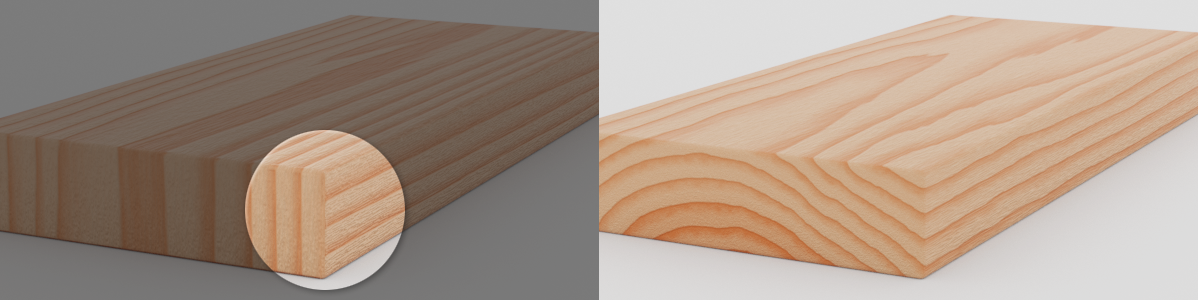
\includegraphics[width=\textwidth]{img/theory/PlaneOrNotAPlane.png}
    \caption{Left$:$ Using a bitmap texture can result in visible seams between object faces as it is inherently difficult to naturally map a 2D texture onto a 3D object. Right$:$ A similar texture rendered with a procedural model. As procedural textures are functions of an objects 3D coordinates, a seamless result is achieved \cite{_comparison}.}
    \label{fig:BitmapVsProcedural}
\end{figure}

\section{Goal}

To alleviate the problems of creating complex procedural texture models by hand, our goal is to develop a \textit{Differentiable Procedural Texture Renderer} or DiPTeR, which can render procedural textures in OpenGL but include a fully differentiable back-end renderer to mimic the rendering process in OpenGL. The back-end renderer should be written in a framework that allows for automatic differentiation, allowing us to create procedural functions and rendering procedures of arbitrary complexity while retaining differentiability. The framework should include a node editor, much like Blender and Substance Designer, that lets users easily build procedural texture models and see their rendered results in real time. A user should be able to present a target bitmap texture, and let the system automatically estimate the optimal parameter values of their procedural texture setup. This means that automatically building a node graph that can render the target image is outside the scope of this project, and is an entirely different problem on its own. Measuring similarity between rendered texture and target texture is done with the means of loss functions, and the framework should allow the user to easily select and implement their own loss functions. While the framework is intended to be operated through a graphical interface developed by us, it should be possible to run the entire texture matching algorithm through a non-graphic user interface.

Through evaluation of our system, we would like to answer the following research questions: Is it possible to build an efficient, differentiable rendering system in PyTorch? Can we achieve an acceptable parameter estimation for a complex procedural texture? Is it fast enough to be usable? Can we find a loss function that performs well in the general case?

\section{Methodology}

Our DiPTeR framework mainly consists of two fairly disconnected parts; the forward user-facing rendering and the backward hidden rendering. The forward rendering is implemented in the popular computer graphics standard OpenGL using python code bindings. All procedural shaders are implemented as fragment shaders written in GLSL, see section \ref{sec:RenderingInOpenGL}. As OpenGL or GLSL doesn't actually have any support for compositing shaders or reusing code, that functionality has been implemented by ourselves, see sections \ref{sec:CompositeShaders} and \ref{sec:ImportPreprocessorDirective} respectively. The backwards rendering is built from scratch in \textit{PyTorch}, a machine learning framework developed by Facebook which includes an automatic differentiation package, As it is a vital component of modern machine learning \cite{paszke_2019_pytorch}. Our backward rendering process is fully differentiable as long as its implemented in the PyTorch ecosystem, and can be used to estimate our forward parameters if implemented to mimic the forward process as closely as possible. One drawback, however, is that PyTorch is not optimized for computer graphics but implementing our procedural shaders as functions of matrices results in adequate performance, and our users will only see the effects of the backwards rendering when running texture matching.

To assists users in designing procedural shaders and see the effects of their choices in real time, we develop a graphical user interface using \textit{PyQt5}, a Python binding for the modern C++ interface library \textit{Qt} \cite{theqtcompany_qt}. Most notibly, we develop a node editor where nodes represent procedural functions that can be composed by connecting nodes' input and output \textbf{REF image?}. We also develop a texture matching interface where a user can select a target image and run our algorithm to automatically estimate parameters of the composed shader function. We use stochastic gradient descent for parameter optimization in our our texture matching algorithm, and PyTorch, being a machine learning framework, proves to be a good choice as it has built in support for Loss functions and Optimizers.

\textbf{Finish with describing evaluation, how data was collected. Did we do user tests? What data was collected?}

\section{Contributions}
\textit{Specify your contributions. What does this particular work/report bring to the research or to the body of knowledge?}

\begin{enumerate}
    \item Using old techniques in new ways = Gradient Descent for inverse rendering. 
    \item Implementing an inverse procedural texture renderer. (even if this is done in pytorch 3d)
    \item Comparison of loss function and optimizers that work best for this task
    \item Ability to easily implement new shaders as well as connecting shaders into compound shaders that are still fully differentiable.
\end{enumerate}

\section{Report outline}

\textbf{Save to last and describe the format and structure of the report.}

% \section{Background}
% \newlist{todolist}{itemize}{2}
% \setlist[todolist]{label=$\square$}
% \begin{todolist}
%     \item Describe why it is not possible to inverse render the existing frameworks, like substance designer or blender!
%     \item Beskriv inverse graphics!
%     \item Mention popular tools that enable use of procedural generation (Blender, 3Ds max, Substance Designer
%     \begin{enumerate}
%         \item Substance designer is popular, but has one large problem in that it only renders to an image. This can be very useful, but isn't tied in to the whole rendering process as well as the other tools, and you can't animate stuffz I think.
%         \item Blender and 3DS max are parts of a whole workflow, but complicated and hard to use. 
%     \end{enumerate}
%     \item[\done]Why are procedural texture hard to work with
%     \item[\done]Why not image synthesis? What is it?
%     \item[\done]resolution independent!
% \end{todolist}

% Procedural generation of data is a concept that has been around for a while and refers to the algorithmic creation of any kind of data and often features a . Procedural generation has gained much popularity in the video game industry, where perhaps the most well known game to feature an extensive use of procedural generation, is Minecraft, where it was used to generate 3D landscapes. The enormous success of Minecraft also boosted the popularity of procedural generation, and saw use in popular titles such as \textit{Teraria}, \textit{Borderlands} and \textit{No Man's Sky}. 


% An alternative to procedural textures is texture synthesis, which has been a popular research subject during the last few years \cite{frhstck_2019_tilegan, zhou_2018_nonstationary}. Texture synthesis takes a sample image as input and aims to create a (possibly infinitely) large output texture with the same pattern and style as the sample image. Current systems can produce results of high quality, but the problem remains in that the input and output are still only bitmap images, which means that they are not very flexible, can result in seams on the mapped 3d object and require even more storage space.

% Procedural textures are a great solution, but there is, of course, a reason why procedural textures have not been widely adopted yet as the de facto standard, and the reason is rather simple: they are difficult to create. In order for an artist to use a bitmap texture of, for example, a type of wood, all that is required is to find a suitable texture image on the web, or simply take their own picture of that object. To create a procedural texture from scratch, an artist would require deep knowledge of both mathematical algorithms and programming. Fortunately, there exists popular tools, like Blender and Substance Designer, to abstract this concept into Node editors, where each node represents a procedural algorithm that can be connected with other algorithms to build a more complex texture. The problem is that this is still very complex. Both applications sport a plethora of different nodes, each of which typically has multiple parameters resulting in many procedural textures having towards a hundred or even more parameters.

% In order to simplify the process, we would like a user to be able to present a target bitmap texture, and let a system decide the appropriate parameter values of a procedural texture setup to match the input image. Essentially we are reversing the rendering process which is usually referred to as \textit{inverse rendering}. Many papers have been written on this topic, but more often than not they focus on other scene parameters like lighting and pose of a 3D object. Not much research has been done that focus on inverse rendering regarding procedural textures and most papers on inverse rendering use machine learning instead of iterative methods. 

% To alleviate the problems of creating complex natural procedural textures by hand, we present DiPTeR, a \textit{Differentiable Procedural Texture Renderer} which uses forward rendering in OpenGL, but sports a fully differentiable back-end renderer written in PyTorch to mimic the rendering process in OpenGL.


% \begin{figure}[!h]
%     \centering
%     \begin{subfigure}[t]{0.40\textwidth}
%         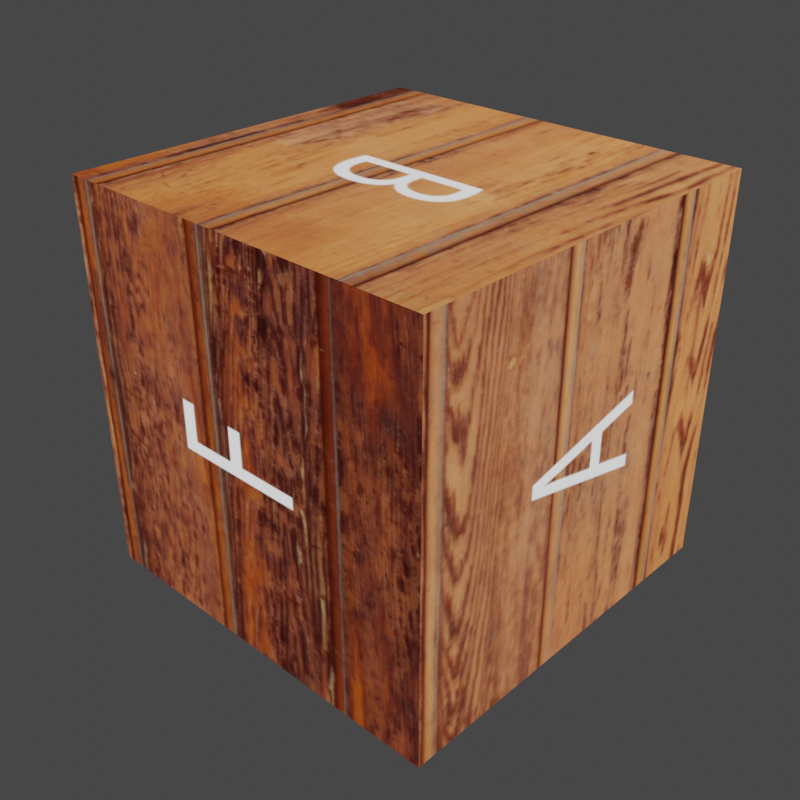
\includegraphics[width=\textwidth]{img/introduction/bad_uv_unwrapping_causes_seams.png}
%         \caption{Example of bad UV mapping which causes visible seams between the faces marked B-A and B-F.}
%         \label{fig:bad-uv-mapping}
%     \end{subfigure}
%     \hfill
%     \begin{subfigure}[t]{0.55\textwidth}
%         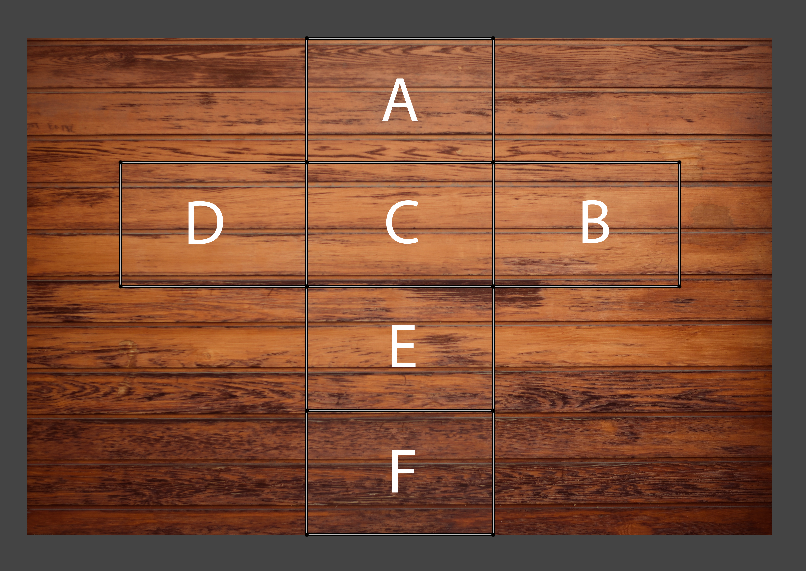
\includegraphics[width=\textwidth]{img/introduction/uv_unwrapping_blender.PNG}
%         \caption{UV unwrapping of the box.}
%         \label{fig:bad-uv-unwrapping}
%     \end{subfigure}
%     \caption{}
%     \label{}
% \end{figure}






\chapter{Background}
\section{Procedural Textures}

Texturing, in general, is a method of adding more detail and realism to a 3D object, traditionally by projecting a 2D bitmap texture to its surface. This is a rather straight forwards process, but presents a number of problems that are difficult to overcome. Firstly, a bitmap texture has a fixed amount of detail; a pixel resolution. The resolution of an image can normally not be scaled up, although new research has made progress in that aspect much thanks to the advances in neural networks \cite{richard_2019_learned, li_2019_a}. However, even if the resolution is sufficient, bitmap textures are still inflexible as it is difficult to modify the underlying pattern without negatively affecting its overall appearance. Furthermore, bitmap textures require a considerable amount of storage space. Another hurdle that is often overlooked, is the inherent problem of projecting 2D texture coordinates $p_{2D} = (u,v)$ onto points on a 3D object's surface $p_{3D} = (x,y,z)$. This mapping process is a function from three dimensional points on an objects surface to two dimensional coordinates in a texture matrix and is often referred to as \textit{UV mapping}, see equation \ref{eq:UVMapping}, often introducing visible seams on the edges between object surfaces as in figure \ref{fig:BitmapVsProcedural}. 

\begin{equation}\label{eq:UVMapping}
    f(u,v) : \mathbb{R}^3 \mapsto \mathbb{N}^2
\end{equation}

Procedural textures are created using mathematical functions, often referred to as \textit{shaders} in computer graphics, that take the surface coordinates of the 3D object as input, as well as a set of $n$ parameters $\theta \in \mathbb{R}^n$ describing its appearance, and returns a color for the point $p_{3D} = (x,y,z)$ see equation \ref{eq:ProceduralMapping}. The parameters $\theta$ can be tweaked by the user to change the underlying patterns and colors, making them much more flexible than the static bitmap approach. 

\begin{equation}\label{eq:ProceduralMapping}
    f(x,y,z,\theta): \mathbb{R}^3, \mathbb{R}^n \mapsto \mathbb{R}^3
\end{equation}


\subsection{Function Composition}

Being functions means we can extend the functionality of procedural textures using \textit{function composition}, a basic mathematical operation taking two functions $f(x)$ and $g(x)$ as input and produces a new function $h(x) = f(g(x))$. While the final output of the procedural texture function should be the color of a point on a target object's surface, any output of any function $g(x)$ can be used as input to a procedural function $f(x)$. To understand how powerful function composition is when user with procedural textures, let $f(\vec{v}, \vec{w}, a)$ be a function of two vectors and a scalar mix factor that returns a weighted sum of both vectors, essentially mixing them. Let $g(x,y,z,a)$ be a function that returns an arbitrary sinusoidal pattern that depends on the input coordinates $(x,y,z)$ as well as a scaling factor $a$ and finally, let $r(x,y,z,\vec{\theta})$ be the main procedural texture function. We also define a red color vector and a green color vector, $c_r = (1.0,0.0,0.0)$ and $c_g = (0.0,0.3,0.0)$ where the elements represent the red, green and blue channels. The functions are defined in equation \ref{eq:ProceduralFunctionComposition} where $\odot$ denotes an element-wise multiplication operation.

\begin{equation}\label{eq:ProceduralFunctionComposition}
\begin{aligned}
    f(\vec{v}, \vec{w}, a) &= \vec{v} \odot (1 - a) + \vec{w} \odot a \\
    g(x,y,z,a) &= \sin(a \cdot x)\cdot \sin(a \cdot y)\cdot \sin(a \cdot z)  \\
    r(x,y,z,\vec{\theta}) &= f(c_r, c_g, g(x,y,z,\theta_0))
\end{aligned}
\end{equation}

Using $r$ as a procedural render function to texture a plane ($\forall z, z = 0$), we achieve 

\subsection{Noise}


\section{Automatic Differentiation}\label{sec:AutomaticDifferentiation}

A major reason why inverse rendering is a difficult problem, is because the rendering process needs to be differentiable in order to be inverted. The reason relates to our iterative optimization algorithm \textit{Gradient Descent}, explained in section \ref{sec:StochasticGradientDescent}, which uses the gradient of a function $f(x_0, x_1, ..., x_i)$, denoted $\nabla f$, defined as the collection of partial derivatives of $f$ with respect to its parameters, see equation \ref{eq:Gradient}. 

\begin{equation}\label{eq:Gradient}
    \nabla f = \begin{bmatrix} \frac{\partial f}{\partial x_0} & \frac{\partial f}{\partial x_1} & \dots & \frac{\partial f}{\partial x_n}\end{bmatrix}
\end{equation}

The rendering process can be seen as one, very convoluted function of many parameters that completely describe a 3D scene, which we need to differentiate. This is completely infeasible in almost all modern renderers like \textit{Blender} or \textit{3Ds Max}, but can be achieved if fully implemented in a framework that allows for \textit{automatic differentiation} such as PyTorch which comes with a very capable \texttt{autograd} package. It should be noted that PyTorch only supports computing gradients for scalar types, so the direct output of a render function, which is likely multi-dimensional, can not be used. However, loss functions are designed to output a single scalar value as a measurement of similarity, and can therefore be used in gradient descent optimization, which is the intended use case of PyTorch's autograd package anyway.

Automatic Differentiation (usually abbreviated AD or \textit{autograd}) is, unsurprisingly, a method of automatically calculating gradients of functions, specifically functions defined in a programming language. Different libraries implement AD in different ways, but almost all work by breaking down complex functions into primitive expressions for which the derivative is known. All other, more complex functions, must be created using these building blocks. How these primitives are applied to input variables and in what order is mapped in a \textit{Computational Graph}, which is the main feature of the AD algorithm.

\subsection{Computational Graph}\label{sec:ComputationalGraph}

\begin{figure}
    \centering
    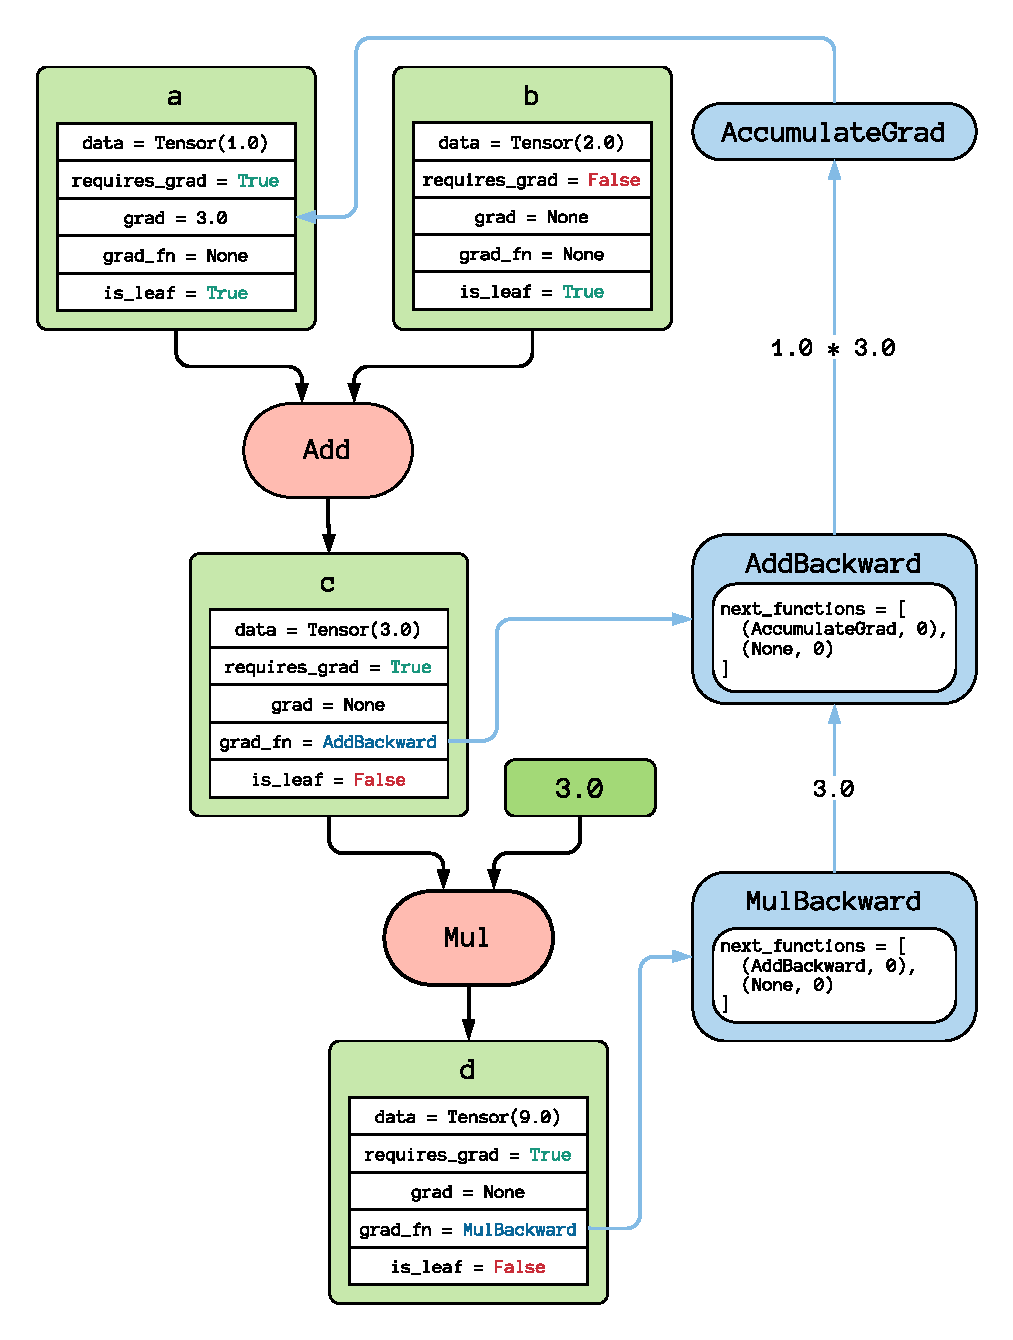
\includegraphics[width=0.9\textwidth]{img/theory/ComputationalGraph.pdf}
    \caption{The computational graph created from the operations in figure \ref{fig:CodeComputationalGraph}. Green nodes represent tensors, red nodes operations and blue nodes the backwards operators that calculate gradients.}
    \label{fig:ComputationalGraph}
\end{figure}

PyTorch operates on its own data structure, called a \codeinline[]{Tensor}, which supports scalars, vectors and matrices of any dimension, much like a Numpy \codeinline[]{ndarray}. Every PyTorch operation performed on a Tensor is registered and added to a directed acyclic graph, usually referred to as a Computational Graph, that tracks the history of computations for that Tensor \cite{autograd}. Each operator in PyTorch extends the \codeinline[python]{Function} class which requires it to implement a \codeinline[python]{forward} and \codeinline[python]{backward} method. The \codeinline[]{forward} performs the operation and the \codeinline[]{backward} method performs the differentiation of the operation. Calling \codeinline[]{backward()} directly on a Tensor will traverse the computational graph in reverse order, using the output of \codeinline[]{backward()} as input to the parent operation, and save the gradient of each participating Tensor in their \codeinline[]{.grad} attribute. An example if shown in figure \ref{fig:ComputationalGraph}, where a few Tensors are created, some operations are performed on them and then the gradient is calculated by calling \codeinline[]{backward()}.

\begin{figure}[h]
    \centering
    \begin{minted}{python}
    a = torch.tensor(1., requires_grad=True)
    b = torch.tensor(2.)
    c = a + b
    d = c * 3.
    d.backward()
    print(d)  # tensor(9.0)
    print(a.grad)  # tensor(3.0)
    \end{minted}
    \caption{}
    \label{fig:CodeComputationalGraph}
\end{figure}

In a way, the backwards traversal of the computational graph is nothing more than a rigorous way of using the standard derivation chain rule, shown in equation \ref{eq:ChainRule}.

\begin{equation}\label{eq:ChainRule}
    \frac{d f(g(x))}{dx} = \frac{d f}{dg} \times \frac{d g}{d x}
\end{equation}

In figure \ref{fig:ComputationalGraph}, we show the computational graph that is created as a result of the operations in \ref{fig:CodeComputationalGraph}. Green color represents Tensor variables, red color represents PyTorch operators while blue color represents everything related to the backward pass that calculates the gradient. Now $\frac{\partial d}{\partial a}$ can automatically be calculated, i.e., the gradient (or more correct the partial derivative) of $d$ with respect to $a$. In the green nodes, the \texttt{requires\_grad} field dictates if a gradient should be computed for this tensor, the \texttt{grad} field contains the calculated gradient value and the \texttt{grad\_fn} contains the backwards version of the last operator used on a tensor. In PyTorch, any tensor explicitly created by the user is called a leaf, denoted by the \texttt{is\_leaf} attribute. Tensors created as a result of operators are not leaves, and PyTorch does not calculate gradients for them. The blue nodes contain a field called \texttt{next\_function} which is a list of tuples that tracks the next backward function to be called. When \texttt{backward()} is called on $d$, the flow backward is started. For Tensors with \codeinline[python]{requires_grad = False} or non-tensors, the next function is None, as we do not need to calculate their gradient. Calculation of the derivative $\frac{d d}{d c} = 3.0$ is already defined in the \texttt{Sum} operator and is passed along to \texttt{AddBackward}. No gradient is passed to tensor $c$ as it is not a leaf. As $b$ has \codeinline[]{requires_grad=False} the next function for $b$ is \texttt{None}. For $a$ however, it is a special function \texttt{AccumulateGrad} that simply accumulates and sets the gradient for $a$. Same as for \texttt{Sum}, \texttt{Add} already contains a definition for its gradient so $\frac{\partial c}{\partial a}$ is easily calculated as $1.0$. Now, according to the chain rule, $\frac{\partial d}{\partial a} = \frac{\partial d}{\partial c} \cdot \frac{\partial c}{\partial a}$, and so we get the product as $1.0 \cdot 3.0$ which is set as the gradient for $a$.

Because PyTorch builds this graph separately for each Tensor, and rebuilds after every call to \texttt{backward()} its possible to use arbitrary Python control flow, like \codeinline[]{for} and \codeinline[]{if} statements, in conjunction with PyTorch operators that can be different for each iteration. This allows us to split our rendering and loss calculations into multiple different processes, as shown in algorithm \ref{alg:GradientDescent}, but still only call \codeinline[]{backward()} on the loss result. Note that this explanation is specific to PyTorch, as not all frameworks implement their computational graph in the exact same way, but most of them follow the same principles.

% \subsection{Vector-Jacobian product}
% The PyTorch operators accept Tensors of arbitrary shape, and so the general case, we want to find the gradient of a \textit{vector valued} function. Given a function $\vec{y} = f(\vec{x})$ where $\vec{x}=(x_0,x_1,...,x_n)$ and $\vec{y} = (y_0,y_1,...,y_m)$ the gradient of $f$ is a so called \textit{Jacobian Matrix}, which is a matrix of all possible partial derivatives of the two vectors $\vec{x}$ and $\vec{y}$, see equation \ref{eq:JacobianMatrix}.

% \begin{equation}\label{eq:JacobianMatrix}
%     \nabla f = J = 
%     \begin{bmatrix} \frac{\partial y_0}{\partial x_0} & \frac{\partial y_0}{\partial x_0} & \dots & \frac{\partial y_0}{\partial x_n} \\ 
%     \frac{\partial y_1}{\partial x_0} & \frac{\partial y_1}{\partial x_1} & \dots & \frac{\partial y_1}{\partial x_n} \\
%     \vdots & \vdots & \ddots & \vdots \\ 
%     \frac{\partial y_m}{\partial x_0} & \frac{\partial y_m}{\partial x_n} & \dots & \frac{\partial y_m}{\partial x_n}
%     \end{bmatrix}
% \end{equation}

% The vector-Jacobian product is the product of a vector $v=(v_0,v_1...v_n)$ and the Jacobian matrix $v^T \cdot J$ and generally, the \texttt{autograd} package of PyTorch is an engine for computing this product.

% Going back to figure \ref{fig:ComputationalGraph}, we call the multiplication operator $mul$ and the addition operator $add$.  We can rewrite rewrite our mathematical notation of $d=(a+b)*3$ in a more programmatical syntax \codeinline[]{d = mul(add(a,b),3)}. To calculate the derivative of $d$, we use the chain rule as shown in equation \ref{}

% \begin{equation}\label{eq:ChainRuleExample}
%     \begin{aligned}
%     \frac{d}{d}mul(add(a,b),3) = \frac{d mul}{d add} \prod \frac{d add}{}
%     \end{aligned}
% \end{equation}

% \textbf{CITE autograd!} \cite{autograd}

\section{Stochastic Gradient Descent}\label{sec:StochasticGradientDescent}

The gradient descent algorithm is one of the cornerstones of this project and is in fact a fairly simple algorithm for iteratively optimizing a, usually, multivariate function. Its most well known use case is in Machine Learning where it is used to minimize the loss of a neural network model. It works by iteratively finding the direction of steepest descent, leading to a minimal value of the loss, defined as the negative of a function's gradient. To find the gradient of a function $f$, it needs to be differentiable which is why our loss function (and each function it depends on) is defined in an auto differentiation framework such as \textit{PyTorch}, see section \ref{sec:AutomaticDifferentiation}.

There are a few major versions of the gradient descent algorithm, the most commonly used in machine learning being mini-batch gradient descent, where the gradient is calculated as an average of multiple samples in order to take a single step. Stochastic gradient descent on the other hand, performs one step for each sample, which is used in our implementation as we only have a single sample (a user's input image). The general algorithm of gradient descent is presented in pseudo-code in algorithm \ref{alg:GradientDescent}. Starting with an arbitrary parameter set $\theta \in \mathbb{R}^n$ which contains all $n$ parameters needed to define an output procedural texture, as well as a loss function $L$ with $\nabla L$ denoting the gradient of $L$ with respect to each parameter in $\theta$, we can update our parameters in each iteration $t$ like shown in equation \ref{eq:GradientDescentUpdate}

\begin{equation}\label{eq:GradientDescentUpdate}
    \begin{aligned}
    v_t = \alpha \cdot \nabla L(\theta_t) \\
    \theta_{t+1} = \theta_t - v_t
    \end{aligned}
\end{equation}

The variable $\alpha \in [0,1]$ is called the learning rate and controls how fast $\theta$ will converge toward the optimal parameter set $\theta^*$ that minimizes our loss function $L$. In general, the gradient descent algorithm solves the optimization problem posed in equation \ref{eq:GradientDescentOptimization}.

\begin{equation}\label{eq:GradientDescentOptimization}
    \argmin_{\theta} L(\theta) = \left\{\theta \mid L(\theta) = \min_{\theta^*} L(\theta^*)\right\}
\end{equation}


The strategy for updating the parameters can be done in much more refined ways using a different \textit{Optimizer}, see section \ref{sec:Optimizer}.  As seen in the algorithm pseudocode and briefly explained in \ref{sec:ComputationalGraph}, we don't actually need the loss to take the set of parameters as input, thanks to the way \textit{PyTorch} registers operations done on any tensor in the set $\theta$ separately for each parameter. 




\begin{algorithm}[H]
\SetKwData{L}{loss}\SetKwData{Iter}{iter}\SetKwData{Truth}{truth}\SetKwData{RenderedImage}{render}
\SetKwFunction{Loss}{Loss}\SetKwFunction{Optimize}{Optimize}\SetKwFunction{Render}{Render}
\SetKwInOut{Input}{Input}\SetKwInOut{Output}{output}

\KwResult{Optimal set of parameters $\mathds{P^*}$ that minimizes loss function \Loss{}}
\Input{The loss goal $l_{goal}$, maximum number of iterations $i_{max}$, and a ground truth image \Truth}

\BlankLine
randomly or strategically initialize $\theta$\;
initialize \Iter $\leftarrow$ $0$\;
\While{\Iter $<$ $i_{max}$}{
    \RenderedImage $\leftarrow$ \Render($\theta$)\;
    \L $\leftarrow$ \Loss{\Truth, \RenderedImage} \;
    \If{\L $\leq$ $l_{goal}$}{
        \Return $\theta$\;
    }
    Backpropagate \L to find the gradient of each parameter in $\theta$\;
    Update $\theta$ according to strategy in optimizer $\theta\leftarrow$\Optimize{$\theta$, $\nabla\theta$}\;
    \Iter $\leftarrow$ \Iter $+1$\;
}
\Return $\theta$\;
\caption{Gradient Descent Algorithm}\label{alg:GradientDescent}
\end{algorithm}


\subsection{Optimizers}\label{sec:Optimizer}

\begin{enumerate}
    \item Insert an image showing SGD oscillating in one direction and the effects momentum has on it, while also explaining why we plot for two variables as a surface plot! \href{https://ruder.io/optimizing-gradient-descent/index.html#gradientdescentoptimizationalgorithms}{LINK}
\end{enumerate}

Optimizers are algorithms describing a strategy for gradient descent to reliably reach the most optimal value of the loss in the fewest amount of steps possible. This is achieved by controlling the updating of the parameters in such a way that we take the largest steps possible towards the optimal value of the loss, without overshooting it or getting stuck in local minima. An analogy of a ball rolling towards the lowest point on a surface (the loss function) in the direction of the downward slope is often used to describe an optimizer's progress. Given a loss function $L$, the most basic optimizer updates each parameter in $\theta$ according to equation \ref{eq:GradientDescentUpdate}. Additionally, for each iteration $t$, the learning rate is usually updated by multiplying it with a decay term $\delta$ so that it diminishes over time. This is to prevent it from overshooting the minimum by forcing it to take smaller steps the closer it gets to the minimum. The drawback of this simple solution, is that it is not very adaptive, and uses the same learning rate for all parameters, thus will give us problems when the derivative differs between parameters. To overcome this, optimizers usually implement something called \textit{momentum}, which adds a fraction $0 \leq \beta \leq 1$ of past update vectors to the current update vector $v_t$. The update steps now become:

\begin{equation}
    \begin{aligned}
    v_t = \beta v_{t-1} + \alpha \cdot \nabla L(\theta) \\
    \theta_{t+1} = \theta_t - v_t
    \end{aligned}
\end{equation}

This is effectively an exponentially weighted moving average, and so for parameters where the gradient is oscillating, this addition will average out those oscillations \textbf{shown in image...}. However, each parameter $\theta_i$ still gets updated using the same learning rate $\alpha$. To battle this, an additional term dubbed \textit{second moment} is calculated, which is a squared weighted average of the past gradients, popularized by \textit{Adagrad} \cite{duchi_2011_adaptive} and refined in \textit{Adadelta} \cite{zeiler_2012_adadelta}. The combination of momentum (first moment) and second moment is used in \textit{Adam} or \textit{Adaptive Moment Estimation}, one of the most popular and successful optimization algorithms used in machine learning \cite{kingma_2014_adam}. The first $m_t$ and second $v_t$ moments for an iteration $t$ are calculated in equation \ref{eq:FirstSecondMoment}.

\begin{equation}\label{eq:FirstSecondMoment}
    \begin{aligned}
    m_t = \beta_1 m_{t-1} + (1-\beta_1) \cdot \nabla L(\theta) \\
    v_t = \beta_2 v_{t-1} + (1 - \beta_2) \cdot \nabla L(\theta)^2
    \end{aligned}
\end{equation}

The two parameters $0 \leq \beta_1, \beta_2 \leq 1$ are used to tune how fast the influence of previous iterations should decay, and is recommended by the authors to be set to $\beta_1 = 0.9$ and $\beta_2 = 0.999$. The second moment, which is a running average of the square of the gradients, controls how much effect the learning rate $\alpha$ has on each parameter $\theta_i$, as shown in equation \ref{eq:Adam}.

\begin{equation}\label{eq:Adam}
    \theta_{t+1} = \theta_t - \frac{\alpha}{\sqrt{v_t} + \epsilon}m_t
\end{equation}

The $\epsilon$ is a small corrective term to prevent division by zero errors. Note that all variables, except $\epsilon$ and $\alpha$ are vectors of size $n$, the number of parameters in $\theta$ and all operations are performed element-wise. Before the first iteration, $m_t$ and $v_t$ are initialized to all zeros, which introduces a bias towards zero for the early iterations. To prevent this, $m_t$ and $v_t$ in equation \ref{eq:Adam} are replaced with their bias corrected versions, $\hat{m}_t$ and $\hat{v}_t$, which are calculated in equation \ref{eq:BiasCorrectedMoments}.

\begin{equation}\label{eq:BiasCorrectedMoments}
    \begin{aligned}
    \hat{m}_t = \frac{m_t}{1- \beta_1^t} \\
    \hat{v}_t = \frac{v_t}{1 - \beta_2^t}
    \end{aligned}
\end{equation}

As the iteration counter $t$ increases, the denominator $1 - \beta^t$ converges towards $1$ and will thus have a negligible effect on the moments in later iterations. Most other optimizers build on these concepts.

\section{Loss functions}

Gradient descent is commonly used to minimize a function that measures the difference between a ground truth $X$, the target, and a generated sample $\hat{X}$, our prediction, as a real number. Such a function is often referred to as a \textit{loss function} or \textit{cost function} as it represents a penalty that we desire to be as small as possible. In our case, we can use it to measure the difference between a user input texture image, our target, and an image that our system has generated. A loss function should output a single scalar value, where larger values represent a bigger difference and a value of zero represent two identical images, at least as measured by the loss function. In general, a loss function could have any input, but our implementations follow what is shown in equation \ref{eq:LossFunctionMapping}, where $L$ denotes a loss function that maps an input of two images matrices $\hat{X}$ and $X$ to a real scalar value. The matrices are real valued and in \textit{column-first} order which is why the width is specified first in $\mathbb{R}^{w \times h \times 3}$, where $w$ and $h$ is the width and height of a rendered image with three color channels.

\begin{equation}
    \begin{aligned}
    L: \hat{X},X \mapsto \mathbb{R} \\
    \text{where } \hat{X}, X \in \mathbb{R}^{w\times h \times 3} \text{ and } w, h \in \mathbb{N}
    \end{aligned}
    \label{eq:LossFunctionMapping}
\end{equation}

The choice of loss function wholly depends on what is being measured. Loss functions for images are a special case, and an entire field of research on its own. Often, it is desired to design a loss function in a way that coincides with a human's perceived difference of two images which can be difficult as the human visual system is very complex. Often simple losses, like MSE explained in section \ref{sec:MeanSquaredError}, are very sensitive to spatial changes in data, which is why more advanced losses are often required.

\subsection{Mean Squared Error}\label{sec:MeanSquaredError}

Mean Squared Error is a popular and simple loss function that measures the squared difference of each pixel, sums them and returns the mean of the sum as shown in equation \ref{eq:MSE}. This kind of loss function is useful if the goal is to reproduce the target image down to the pixel. This is however, not a good representation of how a human would judge the similarity of two images. If target image $X$ and predicted image $\hat{X}$ are identical, except each pixel in $\hat{X}$ is shifted one column to the right, it would still be very hard to distinguish any difference between the two for a human (given a reasonable resolution). Depending on the amount of noise in the image, almost no pixels are identical anymore and we get a large measured difference. This also applies to any scaling, rotation or sheering of images. Thus, MSE has a strong spatial dependency on the compared images. Especially in this project, where procedural textures with high frequency features and patterns is common, we need to look for more sophisticated means of measuring differences between images.

\begin{equation}\label{eq:MSE}
    L_{mse}(\hat{X}, X) = \frac{1}{w\cdot h\cdot 3}\sum_{i,j,c} (\hat{X}_{i,j,c} - X_{i,j,c})^2
\end{equation}

\subsection{Neural Feature Loss}

\begin{enumerate}
    \item Describe how features are extracted and what a gram matrix is...
    \item \textbf{Insert image from lucidchart showing features being extracted...}
    \item Mention that these neural losses are input to MSE.
\end{enumerate}

Developing a reliable method of measuring differences in images is important in inverse graphics as well as machine learning and directly influences its performance. In a way, our algorithm is only as good as our loss function, defining an upper bound on accuracy. In the paper by Guo et. al \cite{guo_2019_a}, several different loss functions are discussed, reaching the conclusion that a loss utilizing features extracted by a neural network such as VGG19 \cite{simonyan_2015_very} performed best. This method is directly adapted from a paper by Gatys et. al. \cite{gatys_2015_texture}, where feature maps $F_i$ are extracted from a few layers of VGG19, and then multiplied together to obtain a \textit{Gram Matrix}. Hu et. al. also used a verion of this as the loss for their neural network model, but calculated histograms on the features instead \cite{hu_2019_a}. Some of these methods are implemented and tested in our project.

\section{Related work}

This thesis primarily cover two topics; Inverse Rendering and Procedural Textures. Neither subjects are new and are both well researched but few papers attempt to combine the two topics. Many approaches at inverse rendering use neural networks, with good results for their somewhat narrow use cases. This thesis was born from inspiration of this method, but it was soon discovered that it is not a viable solution for our use case, where we allow users to freely modify and compose procedural textures, resulting in near endless pattern combinations. Training a neural network to perform well on such data would require an immense dataset to train on, as well as an extremely complex model.

\subsection{Inverse Graphics using Neural Networks}

A popular approach to the inverse graphics problem is using neural networks. Kulkarni et. al propose using a modified Variational Auto Encoder to learn disentangled 3D transformation properties (such as rotation about an axis, or the azimuth of the light source) of a 3D scene \cite{kulkarni_2015_deep}. A \textit{disentangled} representation means that each latent variable $z_i$ in the VAE represents a distinct transformation of the 3D scene. This is achieved, in part, by traning on batches of images where all but one parameter are kept constant. A similar approach is used in a paper by Mahendran et. al, although using a convolutional neural network \cite{mahendran_2017_3d} while a third solution is to use a Generative Adversarial Network that imitates a graphics renderer, which Shi et. al recently did to retrieve parameters for 3D faces from 2D images \cite{shi_2019_facetoparameter}. Neither of these solutions specialize in inverse rendering of textures, but instead a small subset of possible 3D scene parameters or in the case of Shi et. al. a pre-defined set of 3D face parameters. This approach can be adapted for simple pre-defined procedural textures, but is difficult to train on more complex examples. Neural networks also requires a lot of preparation, such as generating training data and requires pre-designed textures and are therefore not a flexible solution.

\subsection{SVBRDF Aquisition}

SVBRDF aquisiton is a popular subsection of inverse graphics for textures that focus on decomposing 2D image textures into spatially-varying bi-directional reflectance distribution functions (SVBRDF for short) maps that describe a texture's roughness, specularity or 3D displacement (normal map) etc. Many papers have in recent years used different neural networks models or image analysis to achieve this \cite{deschaintre_2018_singleimage, kang_2018_efficient, nalbach_2017_deep, aittala_2016_reflectance}. However, instead of finding these maps directly, our thesis focuses on finding the parameters to a procedural texture that allows us to modify it and generate it, albeit only a limited subset of these maps, as we do not consider any 3D displacement or light interaction in this thesis.

\subsection{Texture Synthesis}

Texture synthesis is a very active research area where a sample image is used to create a larger texture with the same pattern and style. Virtually all texture synthesis solutions work with bitmap textures, and thus act as an alternative solution to procedural textures when the goal is to generate varied larger textures from a sample. Solving the inverse problem is not very common, nor is it often needed as it is usually easier to acquire a small texture example of a desired larger version. None the less, Wei et. al. managed to create a framework for inverse texture synthesis, and argued that that it is useful for acquiring a sample from inhomogenous textures \cite{wei_2008_inverse}. Some early solutions to texture synthesis relied on feature extraction and optimization between input and output texture \cite{kwatra_2005_texture}, while others utilized a patch based method where a new image is created by stitching together patches of the original sample \cite{efrosalexeia_2001_image}. As the popularity of neural networks grew, the field of texture synthesis found itself moving away from more manual image analysis solutions and started utilizing CNNs and later GANs. Early on, Gatys et. al. proposed a method for texture synthesis based on extracting features from different levels of a neural network \cite{gatys_2015_texture}. However, recent papers have found that GANs can be used to create high quality results of impressive resolutions. Notably, Früstück et. al. created a framework that supports multiple example images as input to produce a large-scale texture with very little boundary artefacts \cite{frhstck_2019_tilegan}. While texture synthesis can be used to quickly generate high quality output, they are still bound to the pixel space and will thus consume large amounts of storage space and lack the flexibility of being easily modifyable, much like SVBRDF maps.


\subsection{Inverse Procedural Texture Modeling}

This field of computer science is rather specific and a relatively low amount of research has been done on it. Two very recent papers stand out as perhaps the most related work of all, and have been the foundation of this thesis. In 2019, Hu et. al. published \textit{A Novel Framework For Inverse Procedural Texture Modeling} in which they describe a framework for procedural texture model acquisition as well as parameter estimation for said model \cite{hu_2019_a}. A K-means algorithm is used to find the most suitable procedural texture model, among a library of pre-defined models, for a user's input texture. Each procedural texture model has an associated CNN model which is used to solve the regression problem of finding an optimal parameter set to the procedural texture that renders an image close to the users input image. This approach is unfortunately not very flexible, as the procedural textures have to be pre-defined and training a neural network on each texture requires a considerable amount of effort and time. Using CNNs for regression also proved difficult for complex procedural texture models, and so neural networks were abandoned for this thesis altogether. 

A much different approach was formulated in the work by Guo et. al. in 2019, where their solution involves Bayesian inference and sampling of the space of plausible parameters to find an optimal parameter set for a chosen procedural texture \cite{guo_2019_a}. Their solution of an approach implemented in a differentiable framework like \textit{PyTorch} is a direct inspiration, however, in our approach no sampling is needed. Furthermore, they contribute by developing smart loss functions that do not depend on textures being pixelwise aligned which have been implemented in this thesis. One defining differece between their work and ours, is that they do not provide an interface to create procedural textures, and only offers hard-coded procedural textures.

\subsection{Differentiable Rendering}

An important foundation that allows our approach to work is the concept of differentiable rendering, that is, the ability to differentiate the entire rendering process, and thus obtain gradients for it. A few notable examples of this have been an inspiration when we write our own differentiable renderer. Perhaps most notable is the very recently released PyTorch3D, a rendering framework developed by the team behind \textit{PyTorch} \cite{facebookresearch_2020_facebookresearchpytorch3d, paszke_2019_pytorch}. This renderer is in fact implemented in \textit{PyTorch}, making it fully differentiable. This tool was unfortunately released without our knowledge at the same time as this thesis was started, but share many concepts, although their approach is much more general. If time allows, it would be worthwile implementing the rendering of this project in their framework. Earlier approaches like the OpenDR framework is closely related to our project, but with a different focus \cite{loper_2014_opendr}. Similar to our project they create a framework where the entire forward rendering process is differentiable, enabling it to automatically compute scene parameters such as vertex positions, camera parameters and vertex colors. Our solution does not focus on the 3D model or camera parameters, but on per-pixel procedural colors and not only static vertex colors. As much of our algorithm relies on writing differentiable shaders, we must not fail to mention an attempt to do just that, directly implemented in the HLSL shader language \cite{guenter_2011_symbolic}. This project was led by Microsoft Research and although their use case was more aimed towards calculating efficient normals, tangents and derivatives of sub-routines, it remains an interesting idea that sadly would have been too complex to implement in this thesis.

\chapter{Method}
As explained in the background, it is nearly impossible to differentiate the rendering process of a system not built for that purpose, but is a requirement when performing parameter estimation using gradient descent. To combat this, we propose building a back-end renderer in a framework that is automatically differentiable in addition to the normal forward rendering system. If this system is carefully setup to mimic the main forward rendering process, finding optimal parameters to the back-end rendering function will simultaneously solve the problem of finding parameters to the forward rendering function. In the overview of our system shown in Figure \ref{fig:SystemOverview}, these two parts are displayed; the forward rendering framework and a differentiable version used in parameter estimation. The user-facing forward rendering is performed with OpenGL, a popular API for rendering 2D and 3D graphics while the back-end renderer is implemented in Python using PyTorch. To estimate parameters of the functions constituting a procedural texture, the iterative optimization algorithm stochastic gradient descent is used. As explained in section \ref{sec:StochasticGradientDescent} on SGD, this algorithm relies on being able to find gradients of a loss function which in our case, measures the visual difference between a user's input target image and the image rendered from our back-end renderer. To assist users in designing procedural texture models, we have implemented a graphical node editor, where each node keeps a reference to both an OpenGL shader, and an equivalent shader implemented in PyTorch. The resulting node graph is a tree-like data structure that visualizes data flowing from node outputs into node inputs of connected nodes. In this chapter, each part of the system will be explained and motivated in detail, ending with a presentation of our graphical user interface used to control \dipter{}.

\begin{figure}[h]
    \centering
    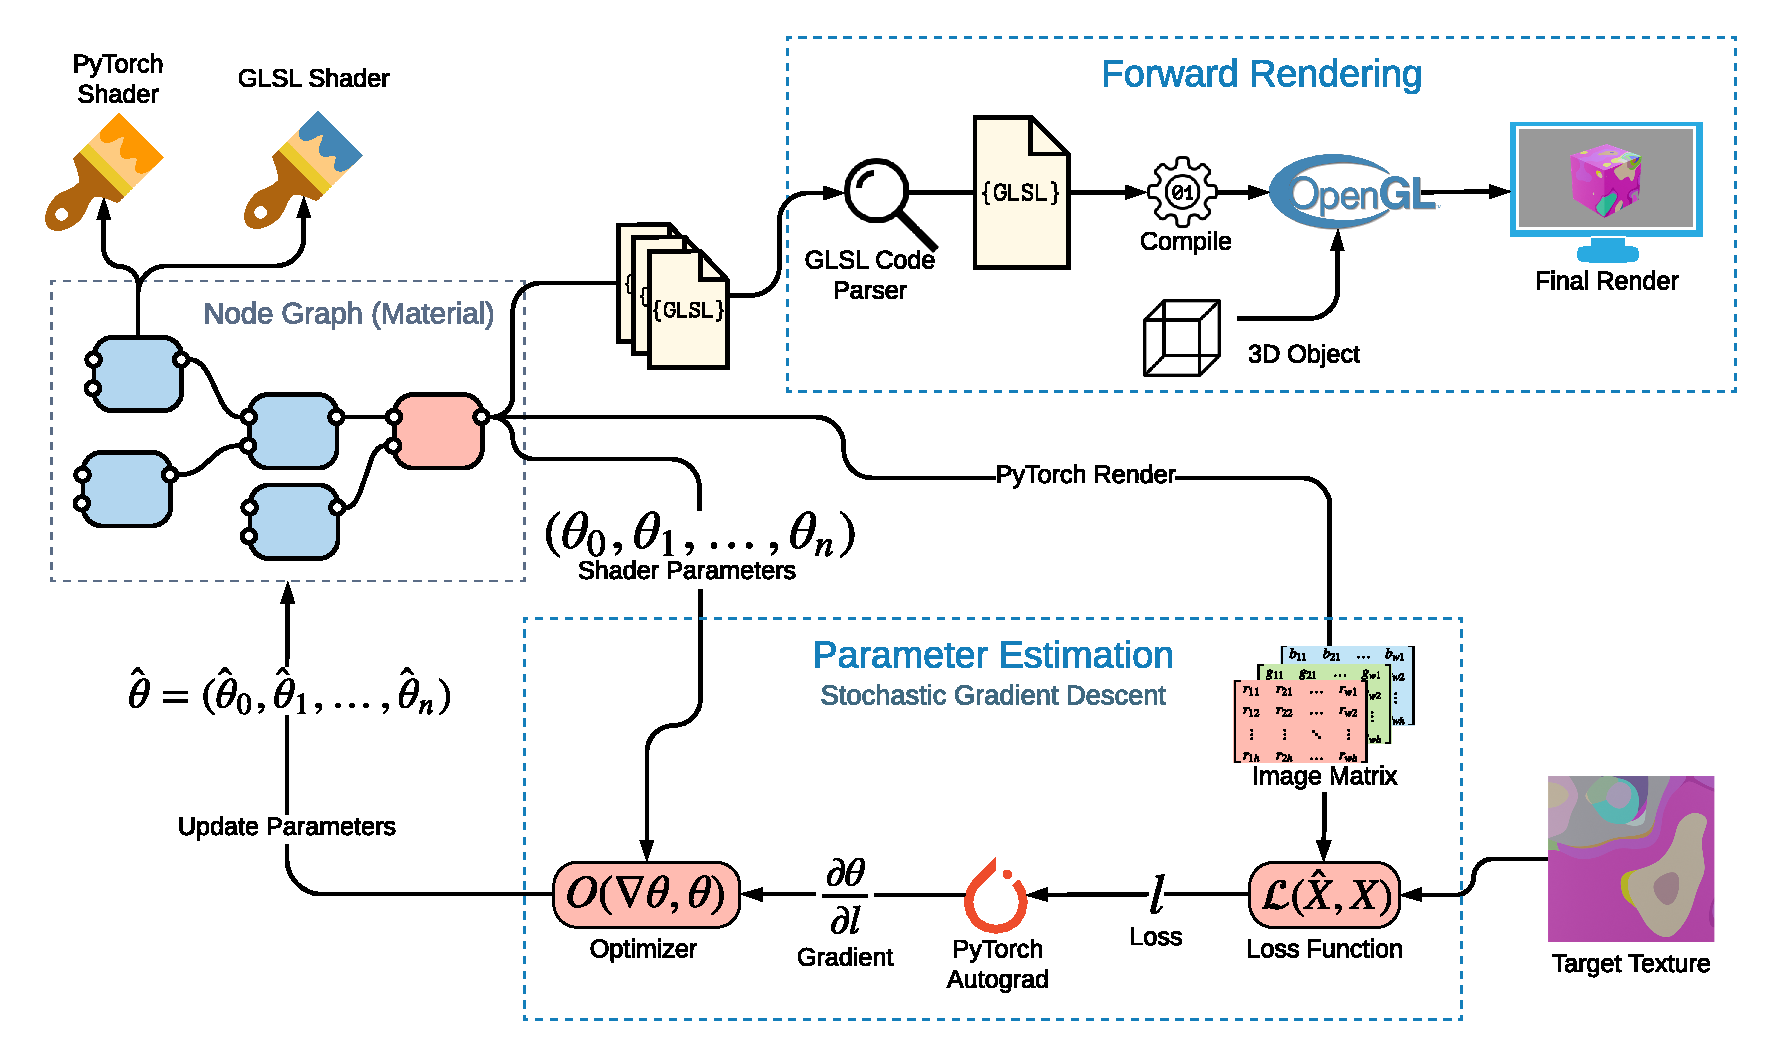
\includegraphics[width=1.0\textwidth]{img/method/System Overview.pdf}
    \caption{Overview of our forward and inverse rendering framework. A user starts by designing a composite shader using the node editor interface. Each node keeps a reference to two versions of the same shader, one for rendering and one for parameter estimation. The GLSL code of each node is parsed, assembled and compiled and sent to OpenGL for rendering. The optional parameter estimation is run in a loop where each iteration, a new rendered image and rendering parameters are used to estimate a better set of parameters, striving to reduce the loss.}
    \label{fig:SystemOverview}
\end{figure}

\section{Node Graph}

Function composition in procedural texturing systems is often illustrated as a node graph, where nodes represent a procedural function. More specifically, this graph is a \textit{directed acyclic graph}, where data flows from the leaf nodes up to the root, the \textit{Material Output Node}, so called because the resulting procedural texture is also referred to as a \textit{material}. The graph is \textit{directed} because data can only flow in one direction, from an output socket into an input socket, and \textit{acyclic} because any nodes connected in a loop would give rise to infinite recursion. An example of such a node graph is illustrated in Figure \ref{fig:NodeGraph}. The root node, a Material Output Node, is a specialized node in \dipter{} for a specific shader called the \textit{material output shader}. This shader acts as the \texttt{main} function in many programming languages, the entry point of execution, as explained in section \ref{sec:ImplementationProceduralShadingGLSL}, and rendering in Python must be initialized from this node. The function accepts one input that the user can not manually set, a color which must be fed from another node.

\begin{figure}[h]
    \centering
    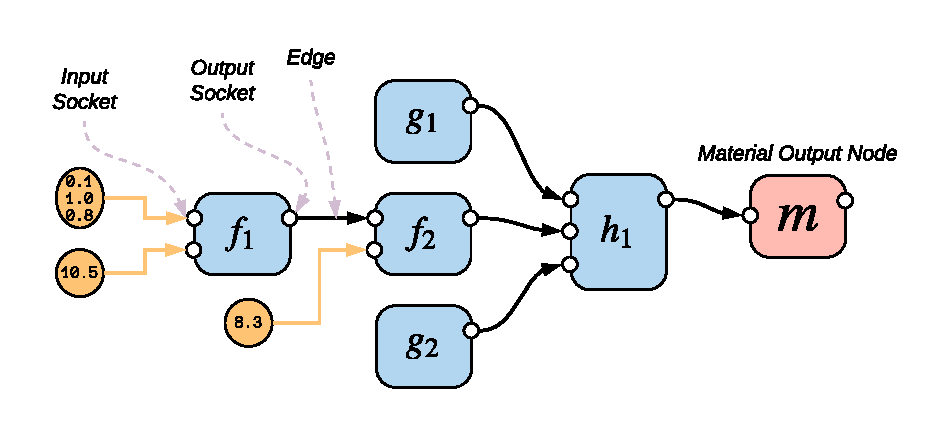
\includegraphics[width=0.9\textwidth]{img/method/Node Graph.pdf}
    \caption{An example procedural texture model represented as a node graph where yellow nodes represent user controlled input. The material output node is the root of the graph, marked in red.}
    \label{fig:NodeGraph}
\end{figure}

The number and type of input sockets of a node are entirely dictated by the shader function it represents and if not connected to another node, can be set by the user. The only exception being the coordinates of the rendered object which is handled internally and is not user controllable. In Figure \ref{fig:NodeGraph} the different functions the nodes represent are printed inside them, where some nodes represent the same function like $f_1$ and $f_2$. The resulting composite procedural texture function $m$ is shown in Equation \ref{eq:NodeGraphCompositeFunction}, omitting the fragment position arguments.

\begin{equation}
    m = h_1(g_1(), f_2(f_1(\left[0.1, 1.0, 0.8\right], 10.5), 8.3), g_2())
    \label{eq:NodeGraphCompositeFunction}
\end{equation}



\section{Forward Rendering}\label{sec:RenderingInOpenGL}

To render procedural textures onto objects we chose OpenGL, a popular and mature graphics API that is fairly easy to set up and integrate into our project. OpenGL comes with all the tools for rendering textures, procedural or not, onto both 2D and 3D objects and is highly optimized for this task. A reasonable question to ask at this point however, is why we even need a separate forward rendering setup at all if our differentiable renderer is designed to render the same result, and the reason is twofold; speed and portability. First of all, our back-end implementation is nowhere near as fast as OpenGL. Even if PyTorch has support for GPU acceleration, the overhead of differentiability and the fact that it is not specifically optimized for graphic computations makes it too slow for real time rendering of anything but the simplest procedural textures, but performs well enough for parameter estimation. In the near future however, this might change as the team behind PyTorch is developing their own differentiable 3D renderer \cite{facebookresearch_2020_facebookresearchpytorch3d}. Lastly, the procedural textures built in our system can be exported and used in any other system that supports shaders written in GLSL. The Python code in our back end is unique to our system, and can not easily be incorporated elsewhere.

\subsection{OpenGL Shader}\label{sec:MethodOpenGLShader}

Procedural textures are rendered in OpenGL using small programs called \textit{shaders}, written in the purpose-built language \textit{OpenGL Shading Language} or GLSL. Details on OpenGL's rendering pipeline, where different types of shaders are explained, can be found in section \ref{sec:OpenGLRenderingPipeline}. \dipter{} mainly deals with fragment shaders which are applied to each fragment or pixel on an object, coloring them according to a function implemented in GLSL. The normalized coordinate of the point on the surface of the 3D object that is covered by the 2D fragment is an important input parameter to the fragment shader. It is calculated by the vertex shader, then interpolated and passed down for each fragment as explained in section \ref{sec:Interpolation}. In our system, this is the sole purpose of vertex shaders, and thus the same vertex shader is used for all types of procedural texture models and only has to be compiled once. Therefore, when we refer to a ''shader'' we refer to the fragment shader. Conceptually, a shader is nothing more than a function applied to each point $p$ on an objects surface that takes a set of optional parameters $\Vec{\theta}$ and the normalized coordinate of $p$ as input, and outputs a color for $p$ calculated from the input parameters, as shown in Figure \ref{fig:OpenGLShader}.


\begin{figure}
    \centering
    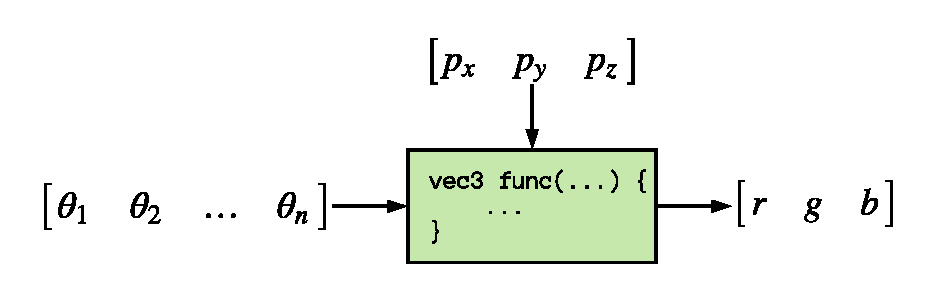
\includegraphics[width=0.9\textwidth]{img/method/Shader Diagram.pdf}
    \caption{A shader in \dipter{}'s forward rendering system is a function, applied to every point $p$ on an objects surface, that takes the normalized coordinate of $p$ and optional parameters $\Vec{\theta}$ as input, and outputs a color vector for $p$.}
    \label{fig:OpenGLShader}
\end{figure}


\subsection{Composing Shaders}\label{sec:MethodComposingShaders}

Much of the power of procedural textures comes from the fact that they are just functions, and as such can be composed and reused as explained in section \ref{sec:BackgroundProceduralTextures}. Unfortunately however, neither OpenGL nor GLSL have any support for shader composition or even code reuse. The latter can fairly easily be supported by implementing a custom preprocessor directive that simply prepends needed source code to a GLSL shader source file before compilation, see section \ref{sec:ImportPreprocessorDirective} on its implementation. Supporting dynamic function composition from Python at run-time however is more complex as GLSL is a compiled language, forcing us to recompile the shader source code each time a change to the node graph's structure is introduced. Furthermore, due to OpenGL restricting us to a single source file for our fragment shader, code from different files need to be assembled into a single file at run-time before compilation. To achieve this, we have built a custom parsing engine that reads and parses GLSL source files once, breaking down files, functions and arguments into Python objects. This code is dynamically reassembled and recompiled according to the structure of the node graph that a user has designed. OpenGL shaders accept input during runtime using so called \textit{uniforms} which have to be uniquely named. This can be tricky when a large node graph is interpreted, as each unconnected node input will be turned into a uniform in the resulting single file source code. If all nodes are of different types this does not pose much of a problem, but as nodes of the same type use the same code (and thus the same underlying argument names), an additional system to ensure unique uniform names is required. Therefore, each node of the same type is assigned a number unique within that type, which the uniform name is based on, see section \ref{sec:ImplementationProceduralShadingGLSL} for details.


\section{Differentiable Rendering}\label{sec:RenderingInDiPTeR}

While designing shaders in OpenGL is fairly easy using GLSL, reusing code and composing shaders dynamically poses a real challenge. For our differentiable shading, the problem is essentially reversed as setting up a rendering system that can reliably mimic the OpenGL renderer is difficult, while composing shaders is trivial and requires no parsing, as dynamically composing functions is innately supported by the Python programming language.

While OpenGL is a fully fledged computer graphics framework, our Python rendering engine is implemented as a simplified and highly specialized differentiable 2D procedural texture rendering engine. No 3D support is needed, as it is only used for parameter estimation by way of 2D texture similarity optimization. Furthermore, it assumes uniform directional lighting, meaning lighting is not calculated as we want to focus on reproducing underlying texture patterns and colors, and parameters governing lighting is not necessarily part of the procedural texture function. By default, OpenGL includes a fourth color channel for opacity which we ignore as it is too ambiguous to be used in inverse rendering and thus handle all images as having three channels.

To be able to differentiate the rendering procedure reliably and dynamically, we need to utilize automatic differentiation. Therefore, we implemented our differentiable renderer using Facebook's machine learning framework \textit{PyTorch} with a built in automatic differentiation engine \cite{paszke_2019_pytorch}. A few other candidates were considered early on, like Google's automatic differentiator \textit{Jax} \cite{bradbury_2018_jax}. This framework has the advantage that it can automatically differentiate code that is almost identical to normal Python or Numpy syntax, whereas most other frameworks require the user to implement code with a specific syntax, a sort of mini-language. Additionally, TensorFlow was temporarily evaluated, but both frameworks were found to be slightly slower and not as robust as PyTorch.

As explained, an important requirement when designing PyTorch shaders is that for a specific parameter set $\Vec{\theta}$ and procedural texture model, both OpenGL and our PyTorch renderer should produce the same 2D texture matrix. Therefore, the simplest way to perform shading would be to iteratively call a shader function, or composition of shader functions, on each pixel of the 2D plane being rendered, mimicking the OpenGL shader in section \ref{sec:MethodOpenGLShader}. This approach in PyTorch is explained in section \ref{sec:MethodIterativeRendering}, but proves very inefficient, why a second much more efficient but unfortunately less readable solution was devised, dubbed \textit{matrix shading}. However, seeing as the rendering times were cut by upward a thousand times, some decrease in readability was deemed a justifiable sacrifice. 


\subsection{PyTorch Shader}

Each OpenGL shader has an associated Python class in \dipter{} which keeps a reference to the GLSL source file. This class will parse the GLSL source code, compile it as well as run tests to ensure compatibility between the two implementations. Additionally, a Python shader class needs to communicate to our system what inputs the shader function accepts and their datatype (used by the node graph subsystem) as well as the actual PyTorch implementation of the GLSL shader function. How the shade function is translated from GLSL into PyTorch's own mini-language is explained in section \ref{sec:ImplementationPyTorchShader}. As in other languages, GLSL comes with a standard library of useful functions that are automatically available when writing shaders and has to be reimplemented in Python. Fortunately, the details behind the mathematical implementation of many of these functions are revealed in the GLSL documentation, but not always. It is therefore important to run tests on each implemented library function to assure that it returns the same result as the GLSL version.

\subsubsection{Generating Fragment Coordinates}

By default convention, the pixel positions in OpenGL are located at \textit{half-pixel coordinates}, meaning that the actual coordinate for a pixel is the position of the center of that pixel \cite{segal_2013_the}. In Python, this means that the index of an element in the rendered image matrix does not directly correlate with the fragment coordinate. This does not matter much if the resolution is high, as the maximum error of the fragment position we can get if we incorrectly assume that the coordinates are given by the lower left corner of a pixel, is half a pixel, or $\frac{1}{2r}$, where $r$ is the pixel resolution in some direction. Let $w$ and $h$ be the image width and height in pixels and $(x,y)$ the index of a pixel element in the matrix, where $0 \leq x \leq w-1$ and $0\leq y \leq h-1$. In general, a pixel's (or fragment's) position at index $(x,y)$ is given by equation \ref{eq:UnnormalizedFragPos}. Note that this is the coordinate in three dimensions.

\begin{equation}\label{eq:UnnormalizedFragPos}
p(x,y) = \begin{bmatrix}x + \frac{1}{2w}, & y + \frac{1}{2h}, & 0\end{bmatrix}
\end{equation}

In our system however, we are only interested in the normalized fragment coordinate, so as to be independent of the rendering resolution. The normalized fragment coordinate \texttt{frag\_pos} is given by equation \ref{eq:FragPos}. Because we need to model our shaders in Python as similar as possible to the OpenGL standard, this is used when generating fragment positions.

\begin{equation}\label{eq:FragPos}
    \fragpos(x,y) = \begin{bmatrix}\frac{x}{w} + \frac{1}{2w}, & \frac{y}{h} + \frac{1}{2h}, & 0\end{bmatrix}
\end{equation}


\subsubsection{Iterative Shading}\label{sec:MethodIterativeRendering}

Iterative shading attempts to model the way shaders operate in OpenGL, where a fragment shader is called for each fragment (effectively pixel) independently and returns a color for that one fragment. To render an image, we first need to define its width and height in pixels and create an empty matrix of shape $(width, height, 3)$ to act as our image placeholder. Then, each position in the matrix is assigned to the output of the render function, where the normalized pixel coordinate \texttt{frag\_pos} is relative to the position in the matrix while the other arguments are kept constant. This algorithm is explained in pseudocode in Algorithm \ref{alg:IterativeRendering}. 

\begin{algorithm}[H]
\SetKwData{Img}{img}\SetKwData{Width}{width}\SetKwData{Height}{height}\SetKwData{Xs}{xs}\SetKwData{Ys}{ys}\SetKwData{X}{x}\SetKwData{Y}{y}\SetKwData{FragPos}{frag\_pos}\SetKwData{Params}{params}
\SetKwFunction{Shade}{Shade}\SetKwFunction{GenerateFragPos}{GenerateFragPos}
\SetKwInOut{Input}{Input}\SetKwInOut{Output}{Output}

\Input{A shade function \Shade, a set of parameters \Params and an image size tuple (\Width, \Height).}
\Output{A matrix of size $\Width \times \Height \times 3$ containing the pixel data for the rendered image.}

\BlankLine
Initialize \Img as empty matrix of size (\Width, \Height, 3)\;

\For {\X $=0$ \KwTo \Width}{
    \For{\Y $=0$ \KwTo \Height}{
        \FragPos $\leftarrow$ \GenerateFragPos{x,y}\;
        \Img[\X, \Y] $\leftarrow$ \Shade{\FragPos, \Params} \;
    }
}
\Return \Img\;
\caption{Iterative rendering algorithm}
\label{alg:IterativeRendering}
\end{algorithm}

While this implementation is straight forward and easily translated from GLSL, the two nested Python for loops become a major performance bottleneck. All PyTorch functions are implemented and highly optimized in a C++ back end while Python for loops are notoriously slow. Furthermore, some shaders do not use the \texttt{frag\_pos} variable, and will thus have the same output for each pixel. Calling the shader function $width \times height$ times, when we could call it once and replicate the output over the entire image, is a huge waste of time. Another, even worse implication is the fact that PyTorch will add a node to the computational graph for each call to a PyTorch function. As such, this approach will add $width \times height$ duplicate operation nodes to the graph, making it much slower to traverse in the backward step as well as memory inefficient. Using only built in functions as far as possible can give a thousandfold performance boost, especially when rendering higher resolution images. How this is achieved is explained in the next section.

\subsubsection{Matrix Shading}\label{sec:MethodMatrixImplementation}

One major disadvantage to PyTorch is that it does not have a \texttt{map}-function that can apply a function to each position in a matrix. This would solve our problem, as we could keep our iterative method while removing the need for slow Python loops. Instead, we can generate input and output parameters for every pixel simultaneously in a matrix the same size as the final rendered image. PyTorch uses its own data structure called a \texttt{Tensor} that represents data of any shape or dimension of any primitive Python type. The functions in the PyTorch library operate on these tensors element-wise, which we can utilize to calculate parameters and color data for the entire image in one call to the shade function. Any parameter of size $d$, be it a scalar where $d=1$ or a color vector where $d=3$, can be extended to a matrix of size $(width, height, d)$ to represent that parameter over the entire image. The fragment coordinates can now be generated once in the superclass, and used by all shaders, as a matrix of size $width, height, d=3)$, where each element is a vector $[p_x,  p_y,  p_z]$. The output of a shader function is now not only the color of a single pixel but the color of all pixels, in other terms; the fully rendered image. Thanks to PyTorch's element-wise operators, the implementation does not have to change at all in some cases, and in most cases, it is only a matter of handling the extra dimensions. The performance gains are particularly significant for shaders that do not utilize the fragment coordinates, and therefore have a uniform color output across the image. In these shaders, the color only have to be calculated once, and then repeated using PyTorch's \texttt{repeat} function, instead of running the shader thousands of times, once for each pixel, like in the iterative method. The other advantage of this method is that the resulting computational graph is much smaller, as each operation only has to be added once.


\begin{equation}\label{eq:FragPosMatrix}
\begin{aligned}
    F[:,:,0] &= 
    \begin{bmatrix} 
        f_x(0,0)    & f_x(1,0)  & \dots     & f_x(w,0)  \\
        f_x(0,1)    & f_x(1,1)  & \dots     & f_x(w,1)  \\
        \vdots      & \vdots    & \ddots    & \vdots    \\
        f_x(0,h)    & f_x(1,h)  & \dots     & f_x(w,h)  
    \end{bmatrix} \\
    F[:,:,1] &= 
    \begin{bmatrix} 
        f_y(0,0)    & f_y(1,0)  & \dots     & f_y(w,0)  \\
        f_y(0,1)    & f_y(1,1)  & \dots     & f_y(w,1)  \\
        \vdots      & \vdots    & \ddots    & \vdots    \\
        f_y(0,h)    & f_y(1,h)  & \dots     & f_y(w,h)  
    \end{bmatrix} \\
    F[:,:,2] &= 
    \begin{bmatrix} 
        0    & 0  & \dots     & 0  \\
        0    & 0  & \dots     & 0  \\
        \vdots      & \vdots    & \ddots    & \vdots    \\
        0    & 0  & \dots     & 0  
    \end{bmatrix}
\end{aligned}
\end{equation}

For visual reference, the fragment coordinates matrix is shown in equation \ref{eq:FragPosMatrix}. Let $f(x,y)$ denote the function that generates the fragment coordinate in equation \ref{eq:FragPos}, at each image integer index $(x,y)$, and let $f_x$, $f_y$, $f_z$ denote the $x$,$y$, and $z$ coordinates returned by $f$, respectively. The equation shows the matrix $F$ that contains all the fragment positions, such that each position $i,j$ in the matrix contains the vector $f(i,j)$. 
The matrix rendering method has an important speed advantage, but there does exist a truly limiting drawback when it comes to loops, where the loop count is dictated by an argument to the shader function. As mentioned, all arguments are matrices, and can therefore not be used as arguments to most Python control flow such as \texttt{if}-statements and \texttt{for}-loops but some of these cases can be solved by using PyTorch alternative functions, see section \ref{sec:ImplementationPyTorchShader}.


% \begin{algorithm}[H]
% \SetKwData{D}{D}\SetKwData{Width}{width}\SetKwData{Height}{height}\SetKwData{T}{t}\SetKwData{V}{V}\SetKwData{FP}{frag\_pos}
% \SetKwFunction{Func}{Func}
% \SetKwInOut{Input}{Input}\SetKwInOut{Output}{Output}

% \Input{A iteration count parameter D.}
% \Output{A rendered image matrix of size $\Width \times \Height \times 3$.}

% \BlankLine
% Initialize V to matrix of zero vectors.\;
% Initialize \FP to fragment coordinates matrix.\;

% \For {\T $=0$ \KwTo \D}{
%     \V = \V + \Func{\FP}\;
    
% }
% \Return \V\;
% \caption{An example of a shader that is very difficult to translate to our matrix form, as \texttt{D} is a matrix with a potentially different value for each pixel, while in an iterative method, the shade function would be executed for each pixel, and \codeinline{D} would simply be an integer scalar tensor.}
% \label{alg:MatrixMethodForProblem}
% \end{algorithm}

\subsection{Composing Shaders}

As Python is our main programming language and the shaders are defined in Python, shaders are already symbolically composed via the node graph. Rendering a composed shader can therefore be easily achieved by traversing the node graph in a correct order and using the output of shaders as input to other connected shaders. Rendering with composite shaders have to be initialized from a node in the graph rather than a shader, as shaders are isolated units, in essence a single function, without any references to other shaders.

The node graph is traversed in depth first order starting from the Material Output root node. Rendering is recursive, and for current node $N$, the algorithm starts by checking each input socket if it is connected and if so, the connected node is recursively rendered and the output is saved to be used as a parameter for $N$s shading function. If the socket is not connected, the parameter value is fetched from the input widget, set by the user in the graphical interface. The unconnected parameters are saved in a dictionary and constitutes the procedural texture parameters $\vec{\theta}$ we want to optimize during parameter estimation. Finally, the shade function is called using the collected parameters and the rendered matrix is returned together with the parameter dictionary for N. For every recursive render call, this dictionary is extended until all connected nodes have been rendered and the parameter dictionary is complete for the graph. This algorithm is shown in Algorithm \ref{alg:PythonCompositeRendering}. The \texttt{Shade} function being called at the end is the shade function of the shader that the current node being rendered contains. The call to \texttt{GetUniqueUniform} is not strictly needed to render an image in Python, but is needed when translating the parameter values to OpenGL in order to know which parameter value belongs to which uniform.


\begin{algorithm}[H]
\SetKwProg{Fn}{Function}{}{end}\SetKwFunction{Render}{Render}%
\SetKwData{Width}{width}\SetKwData{Height}{height}\SetKwData{Arg}{arg}\SetKwData{ParamsDict}{params\_dict}\SetKwData{Arguments}{arguments}\SetKwData{Socket}{socket}\SetKwData{Node}{node}\SetKwData{Value}{value}\SetKwData{PD}{pd}\SetKwData{Uniform}{uniform}\SetKwData{Root}{root\_node}
\SetKwFunction{GetInputSockets}{GetInputSockets}\SetKwFunction{GetConnectedNode}{GetConnectedNode}\SetKwFunction{GetArg}{GetArg}\SetKwFunction{GetValueFromSocket}{GetValueFromSocket}\SetKwFunction{GetUniqueUniform}{GetUniqueUniform}\SetKwFunction{Shade}{Shade}


\Fn{\Render{\Width, \Height}}{
Initialize \ParamsDict as empty dictionary\;
Initialize \Arguments as empty dictionary\;

\For{\Socket $\in$ \GetInputSockets{}}{
    \Arg $\leftarrow$ \GetArg{\Socket}\;
    \Uniform $\leftarrow$ \GetUniqueUniform{\Arg} \;
    \eIf{\Socket is connected}{
        \Node $\leftarrow$ \GetConnectedNode{\Socket}\;
        \tcp{recursive rendering}       
        \Value, \PD $\leftarrow$ \Node.\Render{\Width, \Height}\;
        Update \ParamsDict with \PD\;
    }{
        \Value $\leftarrow$ \GetValueFromSocket{\Socket}\;
        Add \Value to \Arguments with key \Arg\;
    }
    Add \Value to \ParamsDict with key \Uniform \;
}

\Return \Shade{\Arguments}, \ParamsDict \;
}
\caption{Recursive rendering algorithm for composite Python shaders.}
\label{alg:PythonCompositeRendering}
\end{algorithm}




% \section{Testing Shader Implementation Similarity}

% \begin{enumerate}
%     \item We need to ensure that our implementations generate the same results.
%     \item Explain the minimum MSE error we can expect.
% \end{enumerate}

% \textbf{Explain WHAT I did to enable shaders to be composed, not HOW I did it as that's for the implementation chapter...}


\section{Parameter Estimation}

Parameter Estimation, also referred to as \textit{Texture Matching} in \dipter{}, is our subsystem that lets users automatically estimate parameters of a procedural texture model they designed in order to minimize the difference between a target bitmap texture and the procedural texture output. This is posed as an optimization problem as described in equation \ref{eq:GradientDescentOptimization}, where the goal is to find optimal parameters $\Vec{\theta}^*$ such that they minimize a loss function $\loss(\Vec{\theta}^*)$. In our system however, we split the rendering of our procedural texture $\hat{X} = R(\vec{\theta})$ and the loss measurement $l=\loss(\hat{X},X)$ because in PyTorch, all operations performed on Tensors are tracked locally in the Tensor datastructure. This enables us to have the loss function only indirectly depend on the procedural parameters and instead be a function of two parameters, a Python rendered image and a user supplied target image. In other words, we can render the image in one function and calculate the loss in another function, but all operations performed on the parameters in either function will be registered in the Tensors. This is crucial, as it enables us to find the derivative $\frac{\partial \theta_i}{\partial l}$ of any parameter $\theta_i$ in $\vec{\theta}$ with respect to the final loss $l = \loss(\hat{X}, X)$, even though the loss function does not directly depend on parameter $\theta_i$. Parameter estimation is controlled through our texture matching GUI, see section \ref{sec:TextureMatcherInterface}.

\subsection{Loss Functions}\label{sec:MethodLossFunctions}

% \textbf{X and $\hat{X}$ are both clamped before being compared because otherwise they wont correspond to what is being rendered! Both openGL and matplotlib/pyqtgraph clamp values to 0,1.}
We make three loss functions available to users: a simple Mean Squared Error loss, Squared Bin Loss as well as a more sophisticated Neural Loss. The MSE loss function works exactly as described in section \ref{sec:LossFunctions} and is very fast and exact, as it measures similarity between individual pixels. It can perform well for very simple procedural textures where an exactly matching result is possible to obtain. In the general case however, this will not be the case, especially not when noise is used in the textures. The Squared Bin loss function is similar to an MSE loss function, but divides the image into regions or bins of $N\times N$ pixels and calculates the average color of each bin, before finally returning the mean squared error of the averages. This loss function can work well for finding general patterns in an image, but can fail within the regions. Making the regions larger makes it less sensitive to noise, but performs worse within regions, and if the regions are made too small, the loss function will exhibit the same traits as the normal MSE. 

Building on findings by Guo et. al., an even better solution should be to utilize machine learning to automatically unveil the underlying patterns in the textures, and directly comparing them \cite{guo_2019_a}. This type of loss function is dubbed a Neural Loss, as the general idea is to pass the images through a neural network, where image features will be extracted by the different layers in the networks, as explained in section \ref{sec:LossFunctions}. This loss function is much more spatially independent than the other two and should focus more on the general look of the textures. For example, the other two loss functions would be fairly bad at recognizing that two different textures of the same type of wood are similar, because locally, these textures can have very different color values. A neural loss function however, could extract features pertaining to the direction of the grain or the presence of knots etc. A comparison of the performances of these loss functions is found in section \ref{sec:EvalParameterEstimationSpeed}.

\subsection{Gradient Descent}

Gradient Descent is performed much like described in Algorithm \ref{alg:GradientDescent}. Each iteration, an image is rendered using parameters $\vec{\theta}$ and a loss value is calculated between the rendered image $\hat{X}$ and the target image $X$. All operations performed directly on the parameters in $\vec{\theta}$ or on variables created as a result of an operation on a parameter in $\vec{\theta}$ are registered in the computational graph. The next step is to utilize PyTorch's automatic differentiation package to traverse the computational graph backwards from the loss, calculating gradients for each of our parameters. Given the gradients, the direction of the steepest ascent of the loss function relative to each parameter's dimension is known. A small gradient $g_i$ for parameter $\theta_i$ means that only a small correction of this parameter is needed in order to reach an optimal loss value, and vice versa. Lastly, it is up to the chosen optimizer to calculate new values for each parameter based on its gradient. Before the next iteration is started the rendered Python image is updated in the graphical interface and likewise the new parameters are sent to the OpenGL shader program, rendering the updated texture. This is an important visual tool and enables users to verify that the algorithm is correctly optimizing the parameters. Additionally, the new loss value is plotted to display the progress over time. The algorithm terminates when the maximum number of iterations has been reached, or the loss value is less than a specified threshold and the new parameter values can be applied to the procedural texture, if the results are satisfying. 

\section{Graphical User Interface}

While it is possible to build procedural textures and perform parameter estimation programmatically with our framework, it is faster and more convenient to interact with \dipter{} through our graphical user interface. The GUI is created using \textit{PyQt5}, the Python bindings for the popular C++ library \textit{Qt}, an extensive suite for cross-platform embedded and desktop UI development \cite{riverbankcomputing_2020_what,theqtcompany_qt}.

\subsection{Node Editor Interface}\label{sec:NodeEditorInterface}

Node graphs, and thereby procedural textures, are designed by the user in a \textit{node editor interface} shown in Figure \ref{fig:NodeEditorInterface}. This is a graphical user interface that lets users spawn nodes from a menu and drag edges to connect nodes' input and output sockets. Next to an unconnected input socket, a widgets allows users to manually control parameter values of a node's shader. \dipter{} currently supports input values of a number of different types: integer or floating number input, color input by opening a color selector window or scalar vector input. To the right of the node editor is the OpenGL render area, where the procedural shader is rendered onto a chosen object in real time that can be rotated and zoomed by the user and any changes to input values or the structure of the graph will immediately be reflected in the rendering. A menu with available node types can be opened by right clicking the node editor area. Just above the node editor scene is a toolbar where users can create new materials by clicking the \emph{plus} button, as well as select a material to display from the drop-down list. \dipter{} also supports saving and loading materials to JSON format.
 
 
\begin{figure}[!h]
    \centering
    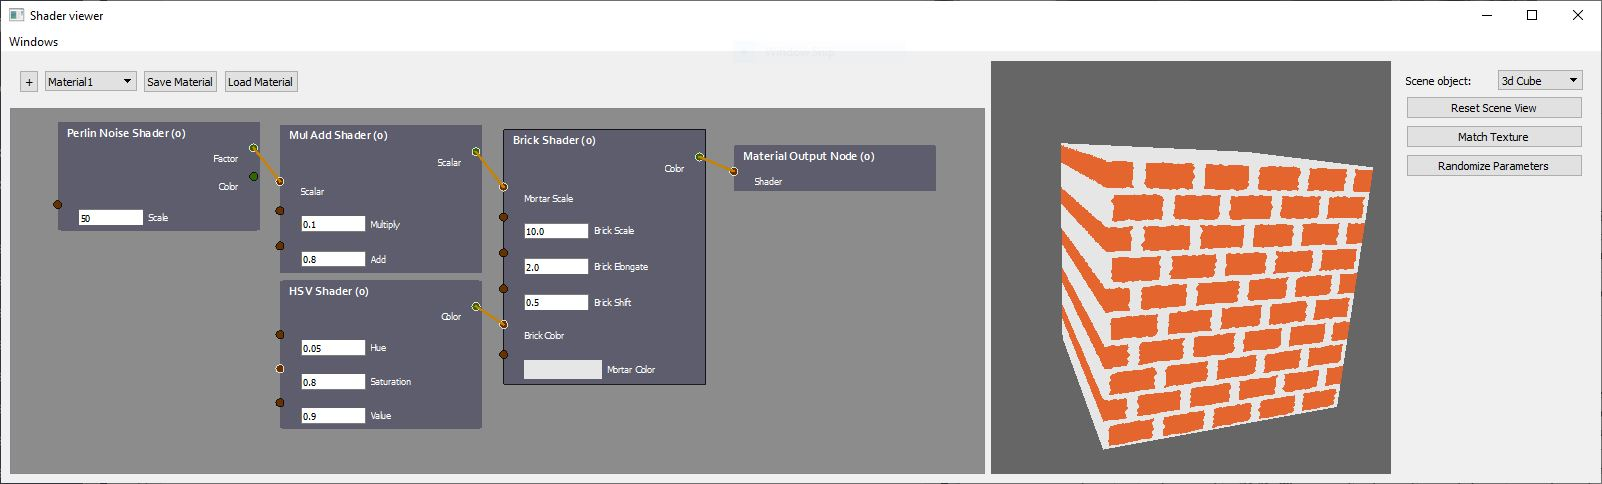
\includegraphics[width=.9\textwidth]{img/method/Node Editor.JPG}
    \caption{Node Editor Interface in \dipter{}. To the right of the node editor is the OpenGL rendering area, where the procedural texture is shown being rendered onto a cube.}
    \label{fig:NodeEditorInterface}
\end{figure}

\subsection{Texture Matcher}\label{sec:TextureMatcherInterface}

Parameter estimation is controlled by the user through our texture matching interface shown in Figure \ref{fig:TextureMatcherInterface}. Here, a user can control various aspects of the gradient descent algorithm such as maximum number of iterations or set a loss threshold that, once reached, signals the completion of the algorithm. Furthermore, the user can select the loss function and optimizer to be used in gradient descent and change their settings. These are the two components that have the largest influence on the success of the parameter estimation process. The loss function sets the upper bound of our result, as a loss of zero is the best outcome we can achieve and if that does not correspond to an optimal similarity between our two images, then the loss function is clearly not good enough. On the other hand, it is the optimizer's job to make sure this value is reached, or at least as close as possible. Apart from the settings panel, the interface is divided into four views. In the top left the procedural texture is shown as rendered by OpenGL, and in the middle, as rendered by the Python back end. Both of these views are updated each iteration and allows the user to assert that the two systems render a similar result and that the algorithm is progressing properly. The top right view displays the target image and hopefully, by the end of the last iteration, all three views will display visually similar images. Lastly, the bottom view plots the loss value versus iteration, hopefully showing a steady decline as the optimization progresses.


\begin{figure}[!h]
    \centering
    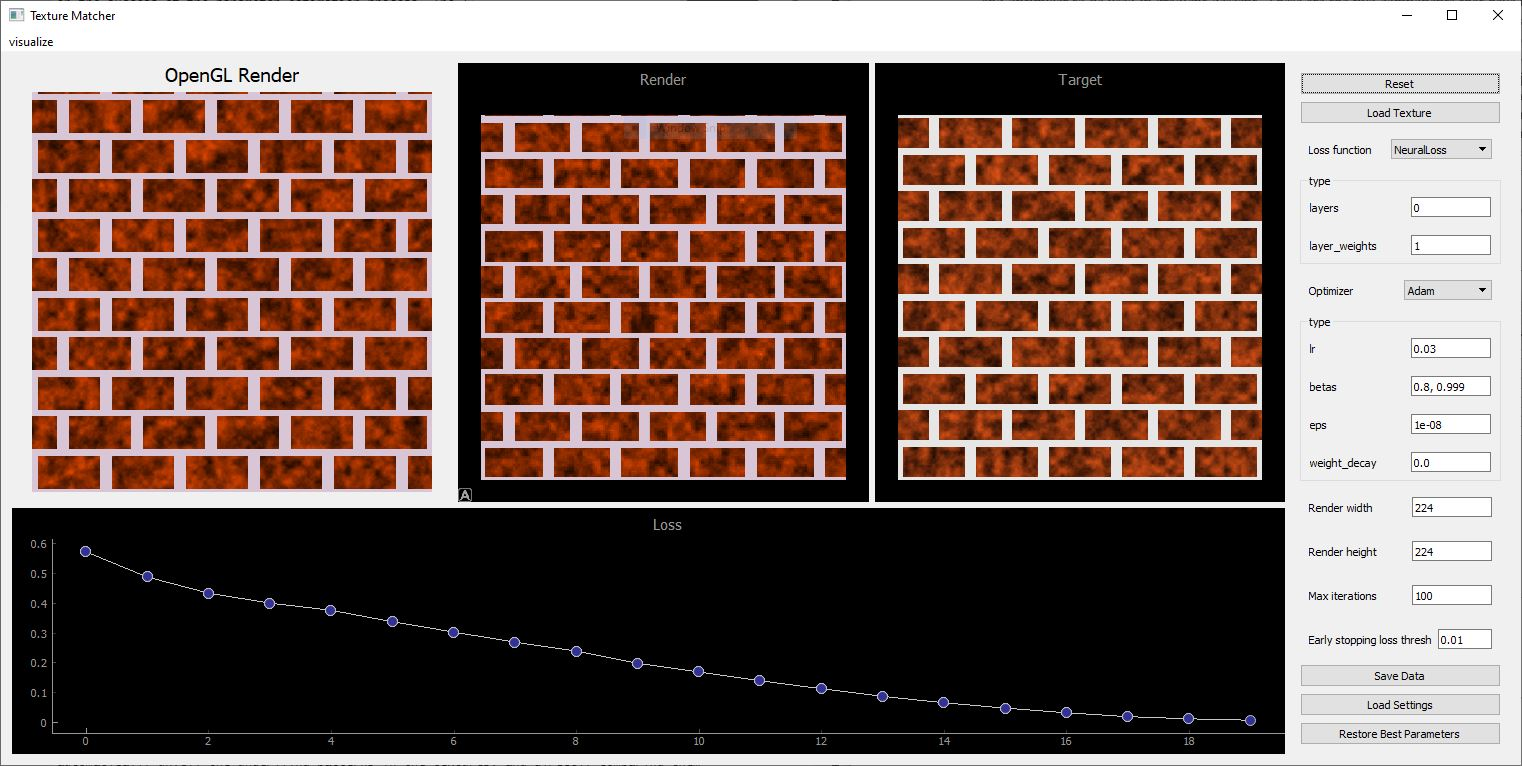
\includegraphics[width=.9\textwidth]{img/method/Texture Matcher.JPG}
    \caption{Graphical interface of the texture matcher, allowing the user to control parameter estimation. The loss has successfully converged to the threshold and all three views show a similar image.}
    \label{fig:TextureMatcherInterface}
\end{figure}

\subsection{Loss Visualizer}\label{sec:LossVisualizerInterface}

The loss value at the end of the gradient descent procedure will almost always be lower than the initial value. However, it is very possible that the final value is a local minima and that a better parameter estimation could be found. One way that this process can be debugged and analyzed is by explicitly plotting the loss for a range of parameter values as a surface plot. Unfortunately, it can only be visualized for two parameters at most, occupying the x- and y-axes, as the third axis is used by the loss value itself. Figure \ref{fig:LossVisualizer} shows the Loss Visualizer interface, where a user can select up to two parameters from their procedural texture in the list on the left and view the resulting, interactive loss surface. A user can also override the minimum and maximum values for each parameter, thereby focusing or restricting the parameter space. From this, it is possible to visually and manually find the optimal loss value relative to the selected parameters. Furthermore, the gradient descent progress can be plotted as a line on top of this surface, allowing the user to see exactly where the algorithm potentially got stuck. In Figure \ref{fig:LossVisualizer} we can clearly see that the gradient descent algorithm, marked with red dots, gets stuck in a local minimum ''valley'' and does not reach the minimum loss marked with a magenta \textit{plus} symbol.

\begin{figure}[!h]
    \centering
    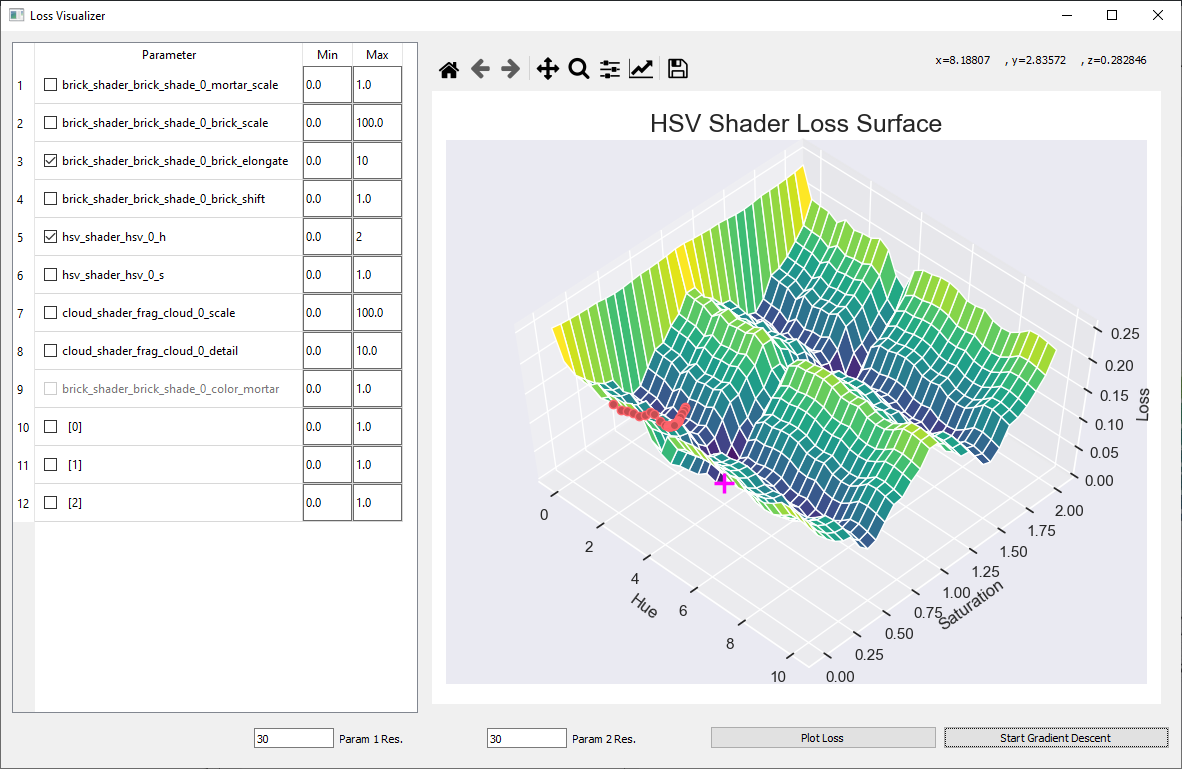
\includegraphics[width=.9\textwidth]{img/method/Loss Visualizer v3.PNG}
    \caption{Loss Visualizer interface showing available parameters and their value ranges to the left and the resulting loss surface to the right. The minimum loss value is marked with a magenta ''plus'' symbol.}
    \label{fig:LossVisualizer}
\end{figure}

\chapter{Implementation}
This chapter outlines the details behind some of the implementation choices in \dipter{}, specifically related to GLSL shader composition and code reuse in section \ref{sec:ImplementationProceduralShadingGLSL}, and how PyTorch shaders were implemented to mimic the GLSL shaders in section \ref{sec:ImplementationPyTorchShader}. Finally, some useful details behind the OpenGL rendering pipeline are presented.

\section{GLSL Shader} \label{sec:ImplementationProceduralShadingGLSL}
 As in many other programming languages, a fragment shader written in GLSL needs a main function as an entry point of execution. However, to simplify shader composition, all shaders in DiPTeR are defined as a single function (but may call other functions), with one exception; the Material Output shader which contains the only \texttt{main} function and must therefore always be the root node in any procedural texture. The different types of shaders in the OpenGL graphics pipeline, see section \ref{sec:OpenGLRenderingPipeline}, are all assembled into a \textit{Program} whose inputs are controlled via parameters called \textit{uniforms}. Each time a new node is connected to the node graph, all the needed code is assembled into one file by our GLSL code parser, where each unconnected parameter of each shader node in the graph is controlled via a uniform. These uniforms, much like any function parameters, need to have unique names which can be partly solved by appending the name of the shader function to the parameter name. However, while the parser ensures that needed function definitions are only inserted once, there are no guarantees that the names of the functions are unique. A modified function name is therefore constructed by also appending the name of the containing source file to the function name and because all shaders are defined in the same folder, this guarantees a unique function name. However, in the case where multiple shader nodes of the same kind are used in a node graph, this is not enough to guarantee a unique uniform name. A \texttt{Material} class is used to add nodes to the node graph as well as assigning a number to each node that is unique among nodes of the same kind. This number is passed to the GLSL code parser responsible for generating the assembled GLSL code and uniforms can now be uniquely named by following the format \texttt{<unique function name>\_<node number>\_<parameter name>}. 
 

% \subsection{Shader Composition} \label{sec:ImplementationShaderComposition}

% \begin{enumerate}
%     \item How is it done in GLSL (recompiling the code)?
%     \item Talk about only one main function, the rest is implemented as simply functions.
%     \item parsing: node number and uniquely naming uniforms.
% \end{enumerate}

\subsection{\texttt{\#import} Preprocessor Directive}\label{sec:ImportPreprocessorDirective}

OpenGL has a number of so called \textit{preprocessor directives}, operators that are processed before shader compilation and are called using the pattern \texttt{\#<name-of-directive> <arguments>}. None of these allow the user to import and reuse code from other files and while this is not a vital function for our project, it is certainly very helpful. Consequently, we implemented our own preprocessor directive called \texttt{\#import} which takes the name of a file to import as an argument. This directive is then parsed by our GLSL parser and the needed files are appended to the code to be compiled. This allows us to call functions from other files as if they were a part of the importing file's definition. 

\section{PyTorch Shader}\label{sec:ImplementationPyTorchShader}

As explained in section \ref{sec:MethodMatrixImplementation}, instead of implementing shading as a process that iteratively renders a texture pixel by pixel, we implement rendering as a function of matrices and render the image all at once. This means that a parameter in GLSL of type \texttt{vec3}, a vector of length 3, corresponds to a \texttt{Tensor} of shape $(W,H,3)$ in Python, where $W$ and $H$ are the width and height of the texture being rendered and the last dimension matches the GLSL parameter type. Unfortunately this implementation is a necessity due to lack of rendering support in PyTorch. While such a solution is immensely faster, it comes with some serious drawbacks in readability that can be mostly fixed with a few tricks that we will describe below, but also a complete lack of support for some important functionality pertaining to control flow in GLSL. Under the hood, all unconnected shader inputs are handled as scalars or vectors and are dynamically converted to matrix form just before rendering, while connected inputs are fetched by rendering from the connected node. 

Ultimately, measuring and confirming the correspondence between the GLSL and PyTorch implementations is done by explicitly measuring the difference between the two frameworks' renders for a variety of parameter combinations. However, it will greatly help the developer to correctly implement shaders in Python if the two languages can utilize similar syntax and call the same functions. To achieve this, we first have to implement parts of the GLSL standard library using PyTorch functions. This can be fairly tricky as the actual source code for the functions are not publicly accessible and may differ between GPU vendors, but some functions have a direct equivalent already implemented in PyTorch, or the mathematical formula for a given function may be revealed by the GLSL documentation. Furthermore, the use of some functions like the \texttt{step} function is problematic as it is not inherently differentiable. We implement it using the \texttt{sign} function as seen below, which is not strictly differentiable either, but can be backpropagated. Note that this and all other PyTorch functions support both scalars, vectors and matrices as all operations used are applied element-wise.

\begin{minted}{python}
def step(edge: Union[float, Tensor], x: Tensor) -> Tensor:
    """
    `step` generates a step function by comparing x to edge.
    For element i of the return value, 0.0 is returned if x[i] < edge[i], 
    and 1.0 is returned otherwise.
    """
    return (torch.sign(x-edge) + 1) / 2
\end{minted}

Next, we demonstrate how the usage of vectors in GLSL can be translated to PyTorch. It is possible to extend the \texttt{Tensor} class in Python, one for each of the vector types in GLSL so that new vectors can be created by for example calling \texttt{vec3(...)}, but this is difficult as the implementation in PyTorch is convoluted, and we do not want to risk breaking the differentiability and portability. Instead, we create a library \texttt{vec.py} to handle the creation of vectors (that are actually matrices), as well as supporting GLSL's syntax of retrieving elements of a vector by calling \texttt{var.x}, \texttt{var.y}, \texttt{var.z} or \texttt{var.w} as well as creating new vectors. In Code \ref{code:HSVGLSL} the GLSL implementation of our HSV shader is shown and in Code \ref{code:HSVPyTorch} the equivalent PyTorch implementation is shown. By implementing the GLSL standard library and the \texttt{vec} library, the implementations can be kept almost identical.

\begin{codefig}
\begin{minted}{glsl}
vec3 hsv(vec3 frag_pos, float h, float s, float v) {
    vec3 c = vec3(h,s,v);
    vec4 K = vec4(1.0, 2.0 / 3.0, 1.0 / 3.0, 3.0);
    vec3 p = abs(fract(c.xxx + K.xyz) * 6.0 - K.www);
    return c.z * mix(K.xxx, clamp(p - K.xxx, 0.0, 1.0), c.y);
}
\end{minted}
\caption{GLSL implementation of the HSV shader function.}
\label{code:HSVGLSL}
\end{codefig}

\begin{codefig}
\begin{minted}{python}
# Import standard GLSL library as gl and vector library vec
from dipter.shaders.lib import glsl_builtins as gl, vec  
def shade_mat(self, h: Tensor, s: Tensor, v: Tensor) -> Tensor:
    c = vec.vec3(h,s,v)
    K = vec.vec4(1.0, 2.0 / 3.0, 1.0 / 3.0, 3.0)
    p = torch.abs(gl.fract(vec.xxx(c) + vec.xyz(K)) * 6.0 - vec.www(K))
    return vec.z(c) * \
        gl.mix(vec.xxx(K), torch.clamp(p - vec.xxx(K), 0.0, 1.0), vec.y(c))
\end{minted}
\caption{PyTorch implementation of the HSV shader function, equivalent to the GLSL implementation in Code \ref{code:HSVGLSL}.}
\label{code:HSVPyTorch}
\end{codefig}

GLSL supports the basic control statements that we are used to in programming like \texttt{while}, \texttt{for} and \texttt{if} statements. One of the flaws with using matrices as parameters becomes obvious if we try to use them in the condition of any Python control flow. For \texttt{if} statements, this can be solved with the PyTorch function \texttt{where} which can evaluate a condition on each position in our matrix, and return a specific value at each position that evaluates to true or another value where it evaluates to false and the only drawback is breaking the syntax conformity. Unfortunately, there is no equivalent function for loops which means we are unable to handle the case where the loop counter is passed from a function argument.

There are a few other discrepancies that need to be managed. Firstly, while a shader in GLSL can utilize a number of different data types such as integers and booleans, the use of such datatypes will break differentiability in PyTorch and we will therefore always work with 32-bit floating point data. In practice however, we can support the use of parameters of any datatype in PyTorch as long as we do not let them be connectable, that is, prohibit the user from connecting such inputs to other nodes. This means that the value of such a parameter must be manually set by the user and are never converted to matrix form. This is utilized, for example, in our \textit{math shader} which returns the result of applying a selected mathematical operator to two values. The mathematical operator, \texttt{+}, \texttt{-}, \texttt{/} or \texttt{*} is selected by comparing the value of an input scalar integer, marked unconnectable and therefore not converted to matrix form, using \texttt{if} statements. The same workaround can be used to address the problem of letting the user control a loop counter, with the only drawback that it will be uniform across the entire texture. Secondly, most implementations of OpenGL supports division by zero, or must at least not lead to an interruption, which differs from Python where division by zero leads to a runtime exception. To remedy this, we add a small float constant to the denominator of any division operations in Python. Finally, the use of bitwise operators are common in GLSL but are only supported for integer types. This is also true for PyTorch, but as integer types are not differentiable the use of bitwise operators in \dipter{} is not possible. Fortunately, it is almost always possible to rewrite code without these operators, possibly at the expense of performance.

% \subsection{Shader Composition}

% \begin{enumerate}
%     \item How is it done in python, how are Tensors tracked and returned so that the same reference is always returned for \texttt{render()}, otherwise backprop will not work...
%     \item Explain that this is possible due to PyTorch only tracking torch operations done on it.
%     \item frag\_pos is calculated once in shader super class...
% \end{enumerate}

% \textbf{Cut from Stochastic Gradient Descent in Background...}
% As seen in the algorithm pseudocode and briefly explained in \ref{sec:ComputationalGraph}, we don't actually need the loss to take the set of parameters as input, thanks to the way \textit{PyTorch} registers operations done on any tensor in the set $\theta$ separately for each parameter. 


\section{Tools}

\subsection{OpenGL Rendering Pipeline}\label{sec:OpenGLRenderingPipeline}

\begin{figure}[!h]
    \centering
    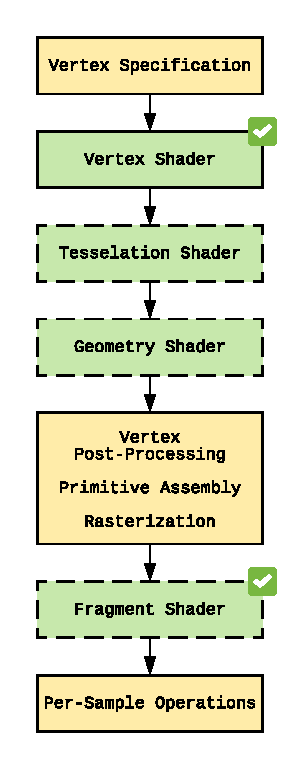
\includegraphics{img/implementation/RenderingPipeline.pdf}
    \caption{An overview of the different stages in the OpenGL Rendering Pipeline. The stages marked green are programmable by user-defined shaders, where the dashed outline marks optional stages, while the yellow stages are controllable through OpenGL function calls. A check mark icon marks the only stages that are used in this project.}
    \label{fig:RenderingPipeline}
\end{figure}

The OpenGL rendering pipeline consists of multiple different stages, defining a workflow starting with 3D vertex data to finally producing 2D pixels on a screen \cite{a2019_rendering}. Some of these stages are programmable by the user, marked in green in Figure \ref{fig:RenderingPipeline}, where the Vertex Shader is the only one \textit{required} to be defined by the user. In the Vertex Specification step, no shader is used, but a list of vertex positions is defined to be rendered as well as a list of triangles that define the faces between these vertices. The Vertex Shader is run on each of these vertices and takes exactly one vertex as input and outputs exactly one vertex. This shader typically also takes three transformation matrices as input that define the scaling, translation and rotation of the object. These are used to output vertices in \textit{clip space} where coordinates are normalized to the interval $[-1,1]$. Next up is the Tesselation Shader and the Geometry Shader. Both manipulate or create geometry but neither are used in our project, as we are only interested in the look of the objects texture, not its geometry. Before the Fragment Shader stage, there is a crucial \textit{rasterization} stage that needs to be completed. This stage turns primitives (like triangles) into fragments, by looping over screen pixels and checking if they lie inside the boundaries of a primitive. If they do, a fragment is created for this pixel and the fragment is given per-vertex values that are interpolated between the vertices that make up the primitive, see section \ref{sec:Interpolation}. The fragments are closely related to screen pixels, but contain more information and each pixel can spawn more than one fragment, depending on multisampling parameters. Each fragment is then sent, one by one, to a Fragment Shader (also called Pixel Shader) which is where all the computations are done that define the final color of a single fragment. In essence, a fragment shader defines a function $f(V,P) \mapsto (r,g,b,a)$ that takes a set of interpolated per-vertex parameters $V$ and a set of user defined parameters $P$ as input, and outputs a fragment color on the form $(r,g,b,a)$, where $r$, $g$, $b$ are the value of the red,green and blue channels, respectively and $a$ is the alpha value of the fragment.

% \subsubsection{Coordinate Systems}\label{sec:CoordinateSystem}

% \textbf{IMAGE EXPLAINING THE DIFFERENT SPACES!} \href{https://learnopengl.com/Getting-started/Coordinate-Systems}{SOURCE}

% In OpenGL there are five different coordinate spaces of interest, and three different transformation matrices that are used to convert between them. The first, \textit{object space}, is the space that is local to a 3D object in the scene. The axes of the local object space are static in relation to the object, no matter how the object is rotated, translated or scaled. As a comparison, a persons left and right will always be the same in relation to that person, but different when compared to another person because it is local to that person. To be able to position object relative to each other, we define a world space. Again, using a real world comparison, this corresponds to the cardinal directions of earth. Moving two objects north on global space, even with different individual local rotations, would move them along the global y-axis. To convert object coordinates to global coordinates, they are multiplied with a matrix often referred to as the \textit{object-to-world} matrix. In OpenGL, we do not need to render everything in the 3D scene, but only what is seen from a camera or viewer's point of view. As such, this space is referred to as view space or camera space. Coordinates in world space are converted to view space with a matrix conveniently referred to as the \textit{world-to-view} matrix. The object are now in a coordinate space that makes sense to the user. Moving an object left to right in view space (along x-axis) will move it left to right on the screen. However, as an OpenGL convention, any vertices outside of the range $[-1,1]$ will be \textit{clipped} or discarded and thus not rendered. Therefore, the next space is referred to as clip space and the coordinates in the range $[-1,1]$ as \textit{Normalized Device Coordinates} or NDC. A user can either define all of its vertices as NDC or in an arbitrary coordinate system and normalize them at this stage. The coordinates are converted from world space to clip space using a \textit{view-to-projection} matrix as the process of converting user defined coordinates to NDC (that are easy to map to a two dimensional coordinate system) is called \textit{projection}. This matrix comes in two forms, depending if \textit{perspective} or \textit{orthographic} projection is used.

% Using the three matrices, it's straight forward to attain the final NDCs in clip space by multiplying the vertices in user defined coordinates with each matrix as seen in equation \ref{eq:ObjectToClipCoordinates}. This defines the required output of the vertex shader, but there is one last important coordinate space to be aware of. This process is called the \textit{viewport transform} and converts the NDCs to screen coordinates, so that each point is mapped to a pixel on the screen. This coordinate system has its origin in the lower left corner of the screen at position $(0,0)$ and runs up to the defined resolution for the OpenGL viewport \textbf{IMAGE SHOWING THIS?}.

% \begin{equation}\label{eq:ObjectToClipCoordinates}
%     V_{clip} = M_{view-to-projection} \cdot M_{world-to-view} \cdot M_{object-to-view} \cdot V_{user}
% \end{equation}


\chapter{Evaluation \& Discussion}
In this chapter the performance of \dipter{} is evaluated by constructing three different test shader models for which rendering speed and parameter estimation accuracy is measured for a number of different combinations of target textures, loss functions and optimizers. All the experiments are performed on a desktop computer with the following specifications:

\begin{itemize}
    \item Operating System: Windows 10
    \item GPU: NVIDIA GeForce GTX 670 2GB
    \item CPU: Intel Core i7 3770K @ 3.50GHz
    \item RAM: 16GB DDR3 @ 667MHz
\end{itemize}

Unfortunately, the version of CUDA supported by this graphics card is too old to utilize PyTorch's GPU accelerated Tensors and thus all operations are performed exclusively on the CPU.

\section{Shader Models for Evaluation}\label{sec:ShaderModelsForEvaluation}

To evaluate \dipter{}, three procedural test shader models of different levels of complexity were created. All models are required to contain a Material Output root node which serves as the output of the shader model. This node does nothing except return the final rendering and will thus be excluded from the explanations of the different node setups. For each shader $M_i$, two textures are rendered: $T_{i1}$ with only two parameters changed from their default values and $T_{i2}$, where each parameter is assigned a random value. These textures are used as targets for our parameter estimation evaluation runs, denoted $X$ in section \ref{sec:LossFunctions} on loss functions. For the last most complex shader model we include an additional real life texture target $T_{33}$ which is not rendered from the shader model itself. 

\subsection{HSV Shader Model $M_1$}
The first shader model, $M_1$ is designed for simplicity using only a single HSV shader node which outputs an RGB color controlled by three values: \textit{hue}, \textit{saturation} and \textit{value}. Consequently, the model depends on a total of three scalar parameters and uses 17 PyTorch functions to render, meaning an equal amount of function nodes make up the resulting computational graph for calculating gradients. The node graph and the rendered texture (using default parameters) are displayed in Figure \ref{fig:M1NodeGraphAndDefaultRender}.

\begin{figure}[!h]
\centering
\begin{tikzpicture}
\node (nodegraph) {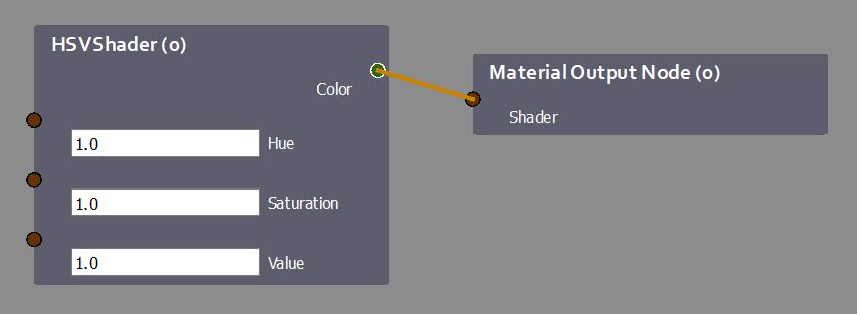
\includegraphics[width=0.7\textwidth]{img/evaluation/Simple HSV Shader Node Graph.JPG}};
\node (render) [right=of nodegraph] {
\includegraphics[width=0.2\textwidth]{img/evaluation/Simple HSV Shader Render.png}};

\draw [ultra thick, ->] (nodegraph) to (render);
\end{tikzpicture}
\caption{HSV test shader $M_1$ using a single HSV Shader node with the rendered texture to the right, using default parameters. The HSV Shader does not utilize the fragment position argument, resulting in a uniformly colored texture.}
\label{fig:M1NodeGraphAndDefaultRender}
\end{figure}

The two generated targets are presented in figures \ref{fig:TargetsHSVShaderModelTwoParam} and \ref{fig:TargetsHSVShaderModelRandom} where the former is rendered by changing only two parameters, the hue and the saturation values, and the latter is rendered by randomizing every parameter.

\begin{figure}[!h]
\centering
\begin{subfigure}{.25\textwidth}
    \centering
    
\includegraphics[width=\linewidth]{img/evaluation/hsv_target_h=0.3,s=0.6.png}
    \caption{Target texture $T_ {11}$ where the hue and saturation values are changed.}
    \label{fig:TargetsHSVShaderModelTwoParam}
\end{subfigure}\hspace{1.5cm}
\begin{subfigure}{.25\textwidth}
    \centering
    
\includegraphics[width=\linewidth]{img/evaluation/hsv_random_target h=0.06,s=0.881,v=0.501.png}
    \caption{Target texture $T_ {12}$ where all parameters have been randomized.}
    \label{fig:TargetsHSVShaderModelRandom}
\end{subfigure}
\caption{The two test target textures for HSV Test Shader model $M_1$.}
\label{fig:TargetsHSVShaderModel}
\end{figure}

\subsection{Simple Brick Shader Model $M_2$}
The next test shader $M_2$ is a basic brick shader with a total of three shader nodes: a cloud shader, HSV shader and a brick shader. The color of the bricks are controlled by a color from the HSV shader, where the \textit{value} parameter is modulated by noise from the cloud shader. The model has a total of 9 user controllable input parameters, one of which is a color vector parameter with three channels, so in reality the model depends on 11 parameters. The brick shader is fairly complex, resulting in a big leap in number of PyTorch functions used, from 17 for $M_1$ to 544 for $M_2$. The brick test shader node graph and resulting rendered texture for default parameters are displayed in Figure \ref{fig:M2NodeGraphAndDefaultRender}.

\begin{figure}[!h]
    \centering
    \begin{tikzpicture}
        \node (nodegraph) {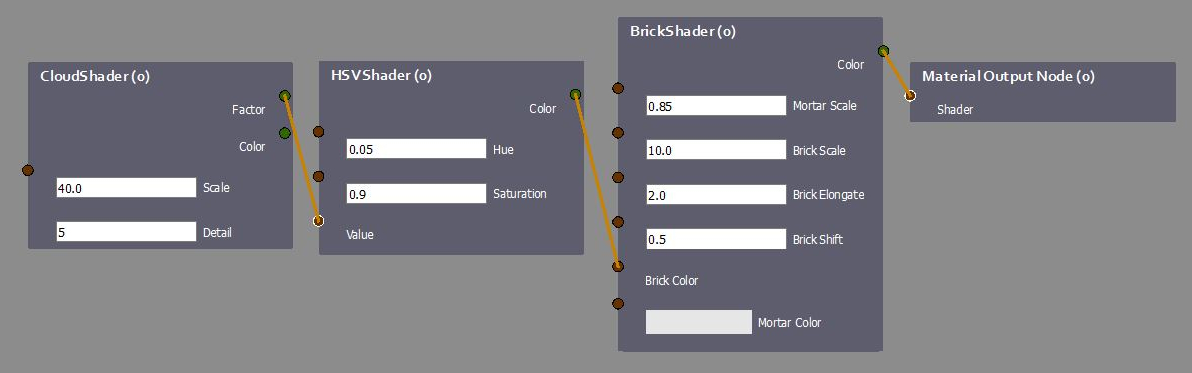
\includegraphics[width=0.7\textwidth]{img/evaluation/Brick Shader Node Graph.JPG}};
        \node (render) [right=of nodegraph] {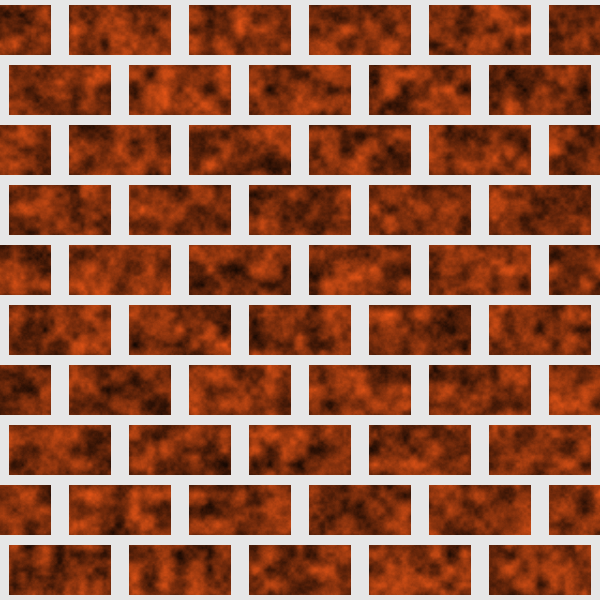
\includegraphics[width=0.2\textwidth]{img/evaluation/Brick Shader Render.png}};
        
        \draw [ultra thick, ->] (nodegraph) to (render);
    \end{tikzpicture}
    \caption{Brick shader $M_2$ using a Cloud Shader connected to a HSV Shader connected to a Brick Shader with the resulting rendered texture to the right, using default parameters. }
    \label{fig:M2NodeGraphAndDefaultRender}
\end{figure}

The two generated targets for $M_2$ are presented in figures \ref{fig:TargetM2TwoParam} and \ref{fig:TargetM2Random} respectively. The first is rendered by changing only two parameters, the elongation of the bricks and the hue of the bricks, and the last is rendered by randomizing every parameter.

\begin{figure}[!h]
\centering
\begin{subfigure}[t]{.25\textwidth}
    \centering
    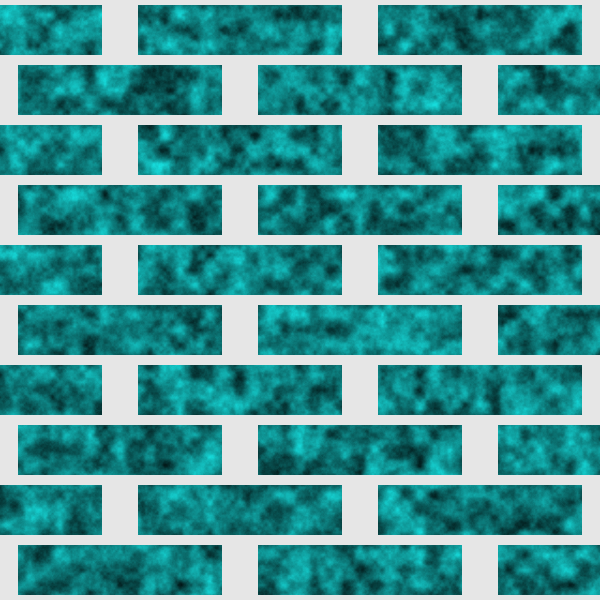
\includegraphics[width=\linewidth]{img/evaluation/simple_brick_target brick_elongate=4,hue=0.5.png}
    \caption{Target texture $T_ {21}$ where the elongation and hue of the bricks are changed.}
    \label{fig:TargetM2TwoParam}
\end{subfigure}\hspace{1.5cm}
\begin{subfigure}[t]{.25\textwidth}
    \centering
    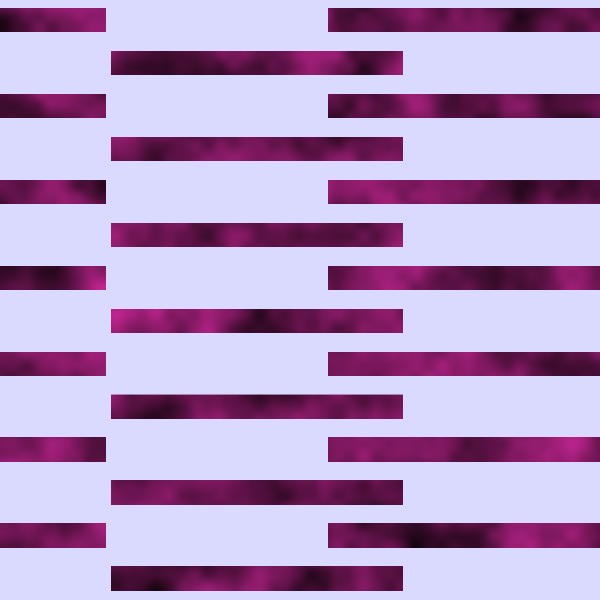
\includegraphics[width=\linewidth]{img/evaluation/simple_brick_random_target.png}
    \caption{Target texture $T_ {22}$ where every parameter is randomized.}
    \label{fig:TargetM2Random}
\end{subfigure}
\caption{The two test target textures for shader model $M_2$.}
\label{fig:TargetsM2}
\end{figure}


\subsection{Advanced Brick Shader Model $M_3$}
The final shader model $M_3$ is an advanced version of $M_2$ using a different brick shader adapted from \textit{Blender's} brick shader implementation in GLSL, as well as using classic 3D perlin noise, which is much more complex than the fractal brownian motion noise used in the cloud shaders. In total, $M_2$ depends on 26 parameters and a total of 2498 PyTorch functions. The node graph of $M_3$ and rendered texture using default parameters are shown in Figure \ref{fig:M3NodeGraphAndDefaultRender}.

\begin{figure}
    \centering
    \begin{tikzpicture}
    \node (nodegraph) {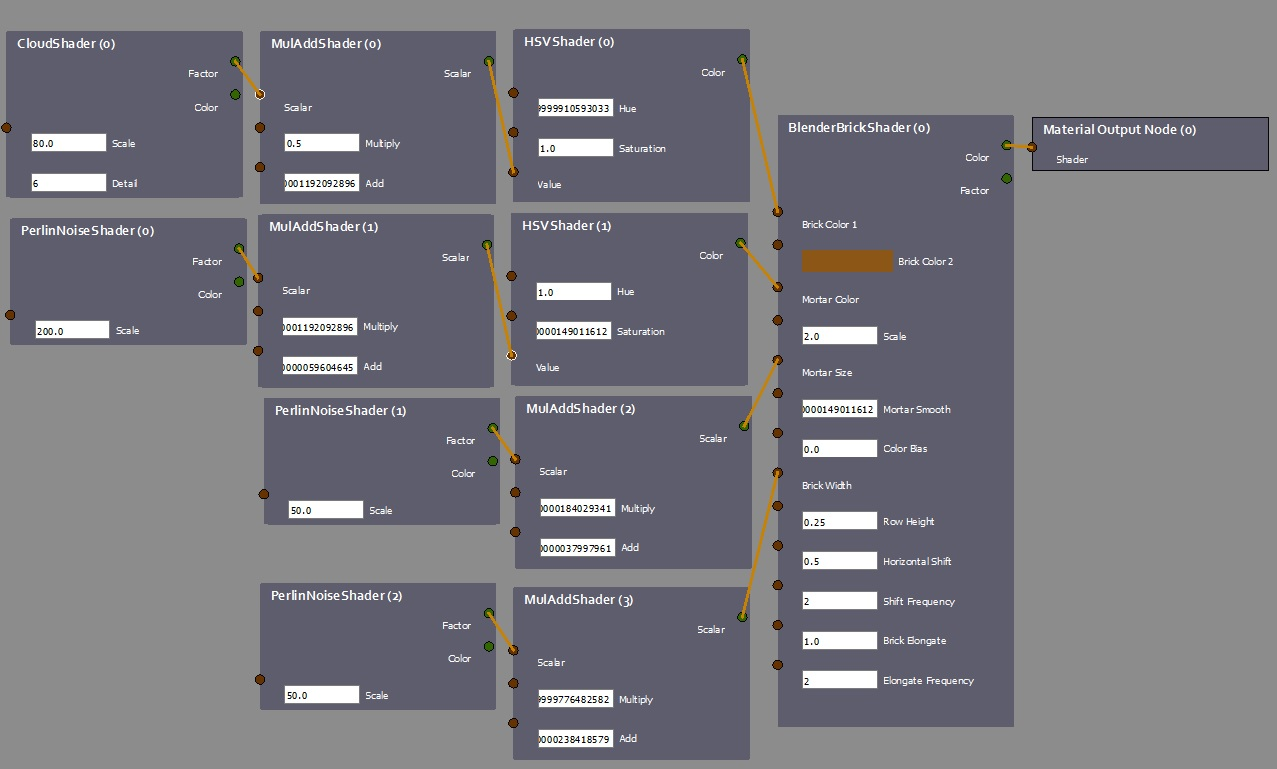
\includegraphics[width=0.7\textwidth]{img/evaluation/Advanced Brick Shader Node Graph.jpg}};
        \node (render) [right=of nodegraph] {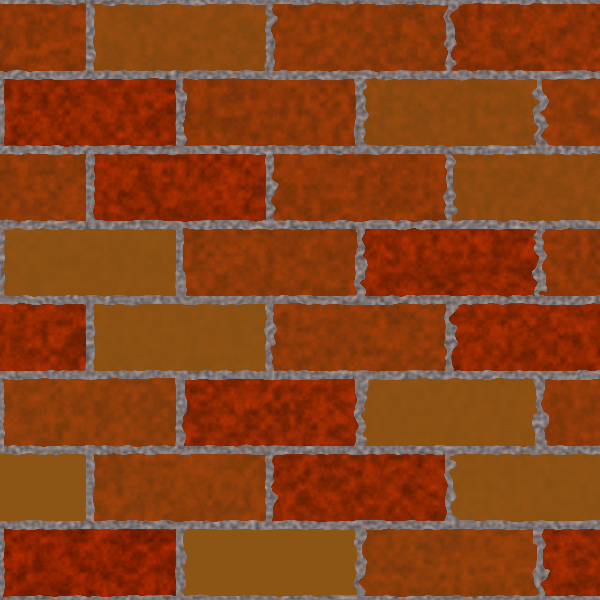
\includegraphics[width=0.2\textwidth]{img/evaluation/Advanced Brick Shader Render.png}};
        
        \draw [ultra thick, ->] (nodegraph) to (render);
    \end{tikzpicture}
    \caption{Advanced brick shader $M_3$ using an adapted version of \textit{Blender's} brick shader as well as multiple instances of classic 3D perlin noise. The resulting rendered texture using default parameters is shown on the right.}
    \label{fig:M3NodeGraphAndDefaultRender}
\end{figure}

For this shader model, we generate two targets in a fashion similar to $M_1$ and $M_2$ shown in figures \ref{fig:TargetM3T31TwoParam} and \ref{fig:TargetM3T32Random} respectively. The first image shows the target rendered by changing only two parameters, the scale of the bricks and the color bias while the second image shows a target rendered by randomizing each parameter. Additionally, this shader is advanced enough that it could render something resembling a real life texture, which is why we test it on a third, real life texture of a brick wall, shown in Figure \ref{fig:TargetM3T33RealLife}.

\begin{figure}[!h]
\centering
\begin{subfigure}[t]{.25\textwidth}
    \centering
    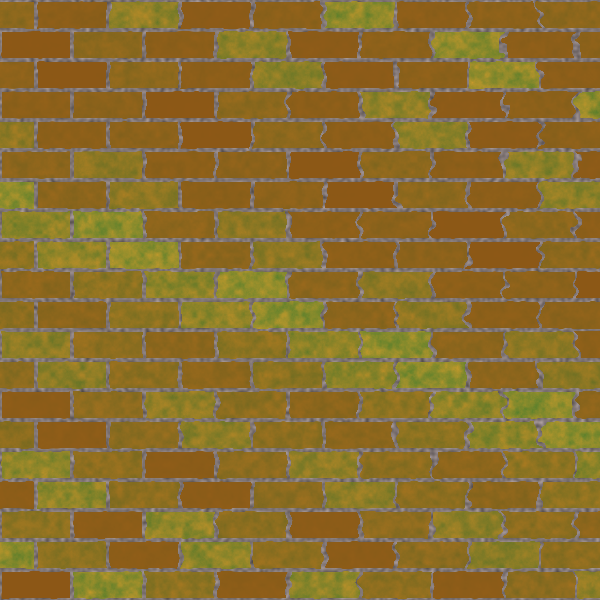
\includegraphics[width=\linewidth]{img/evaluation/adv_brick_target_scale=5,color_bias=1.png}
    \caption{Target texture $T_ {31}$ where the brick scale and color bias have been changed.}
    \label{fig:TargetM3T31TwoParam}
\end{subfigure}\hspace{0.7cm}
\begin{subfigure}[t]{.25\textwidth}
    \centering
    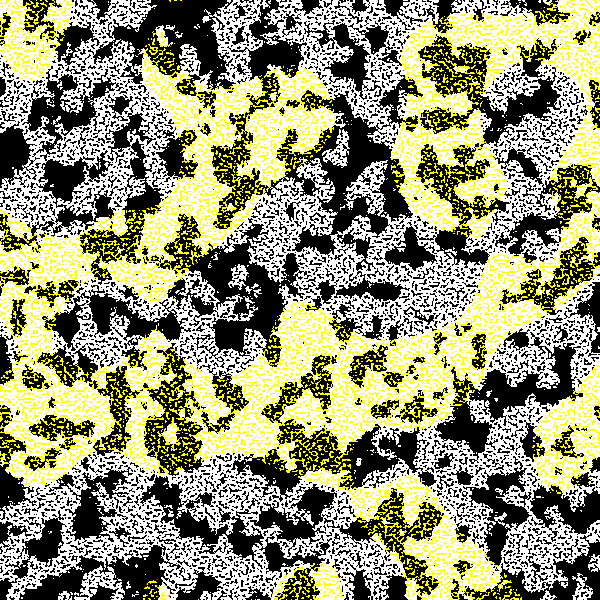
\includegraphics[width=\linewidth]{img/evaluation/adv_brick_random_target.png}
    \caption{Target texture $T_ {32}$where every parameter has been randomized.}
    \label{fig:TargetM3T32Random}
\end{subfigure}\hspace{0.7cm}
\begin{subfigure}[t]{.25\textwidth}
    \centering
    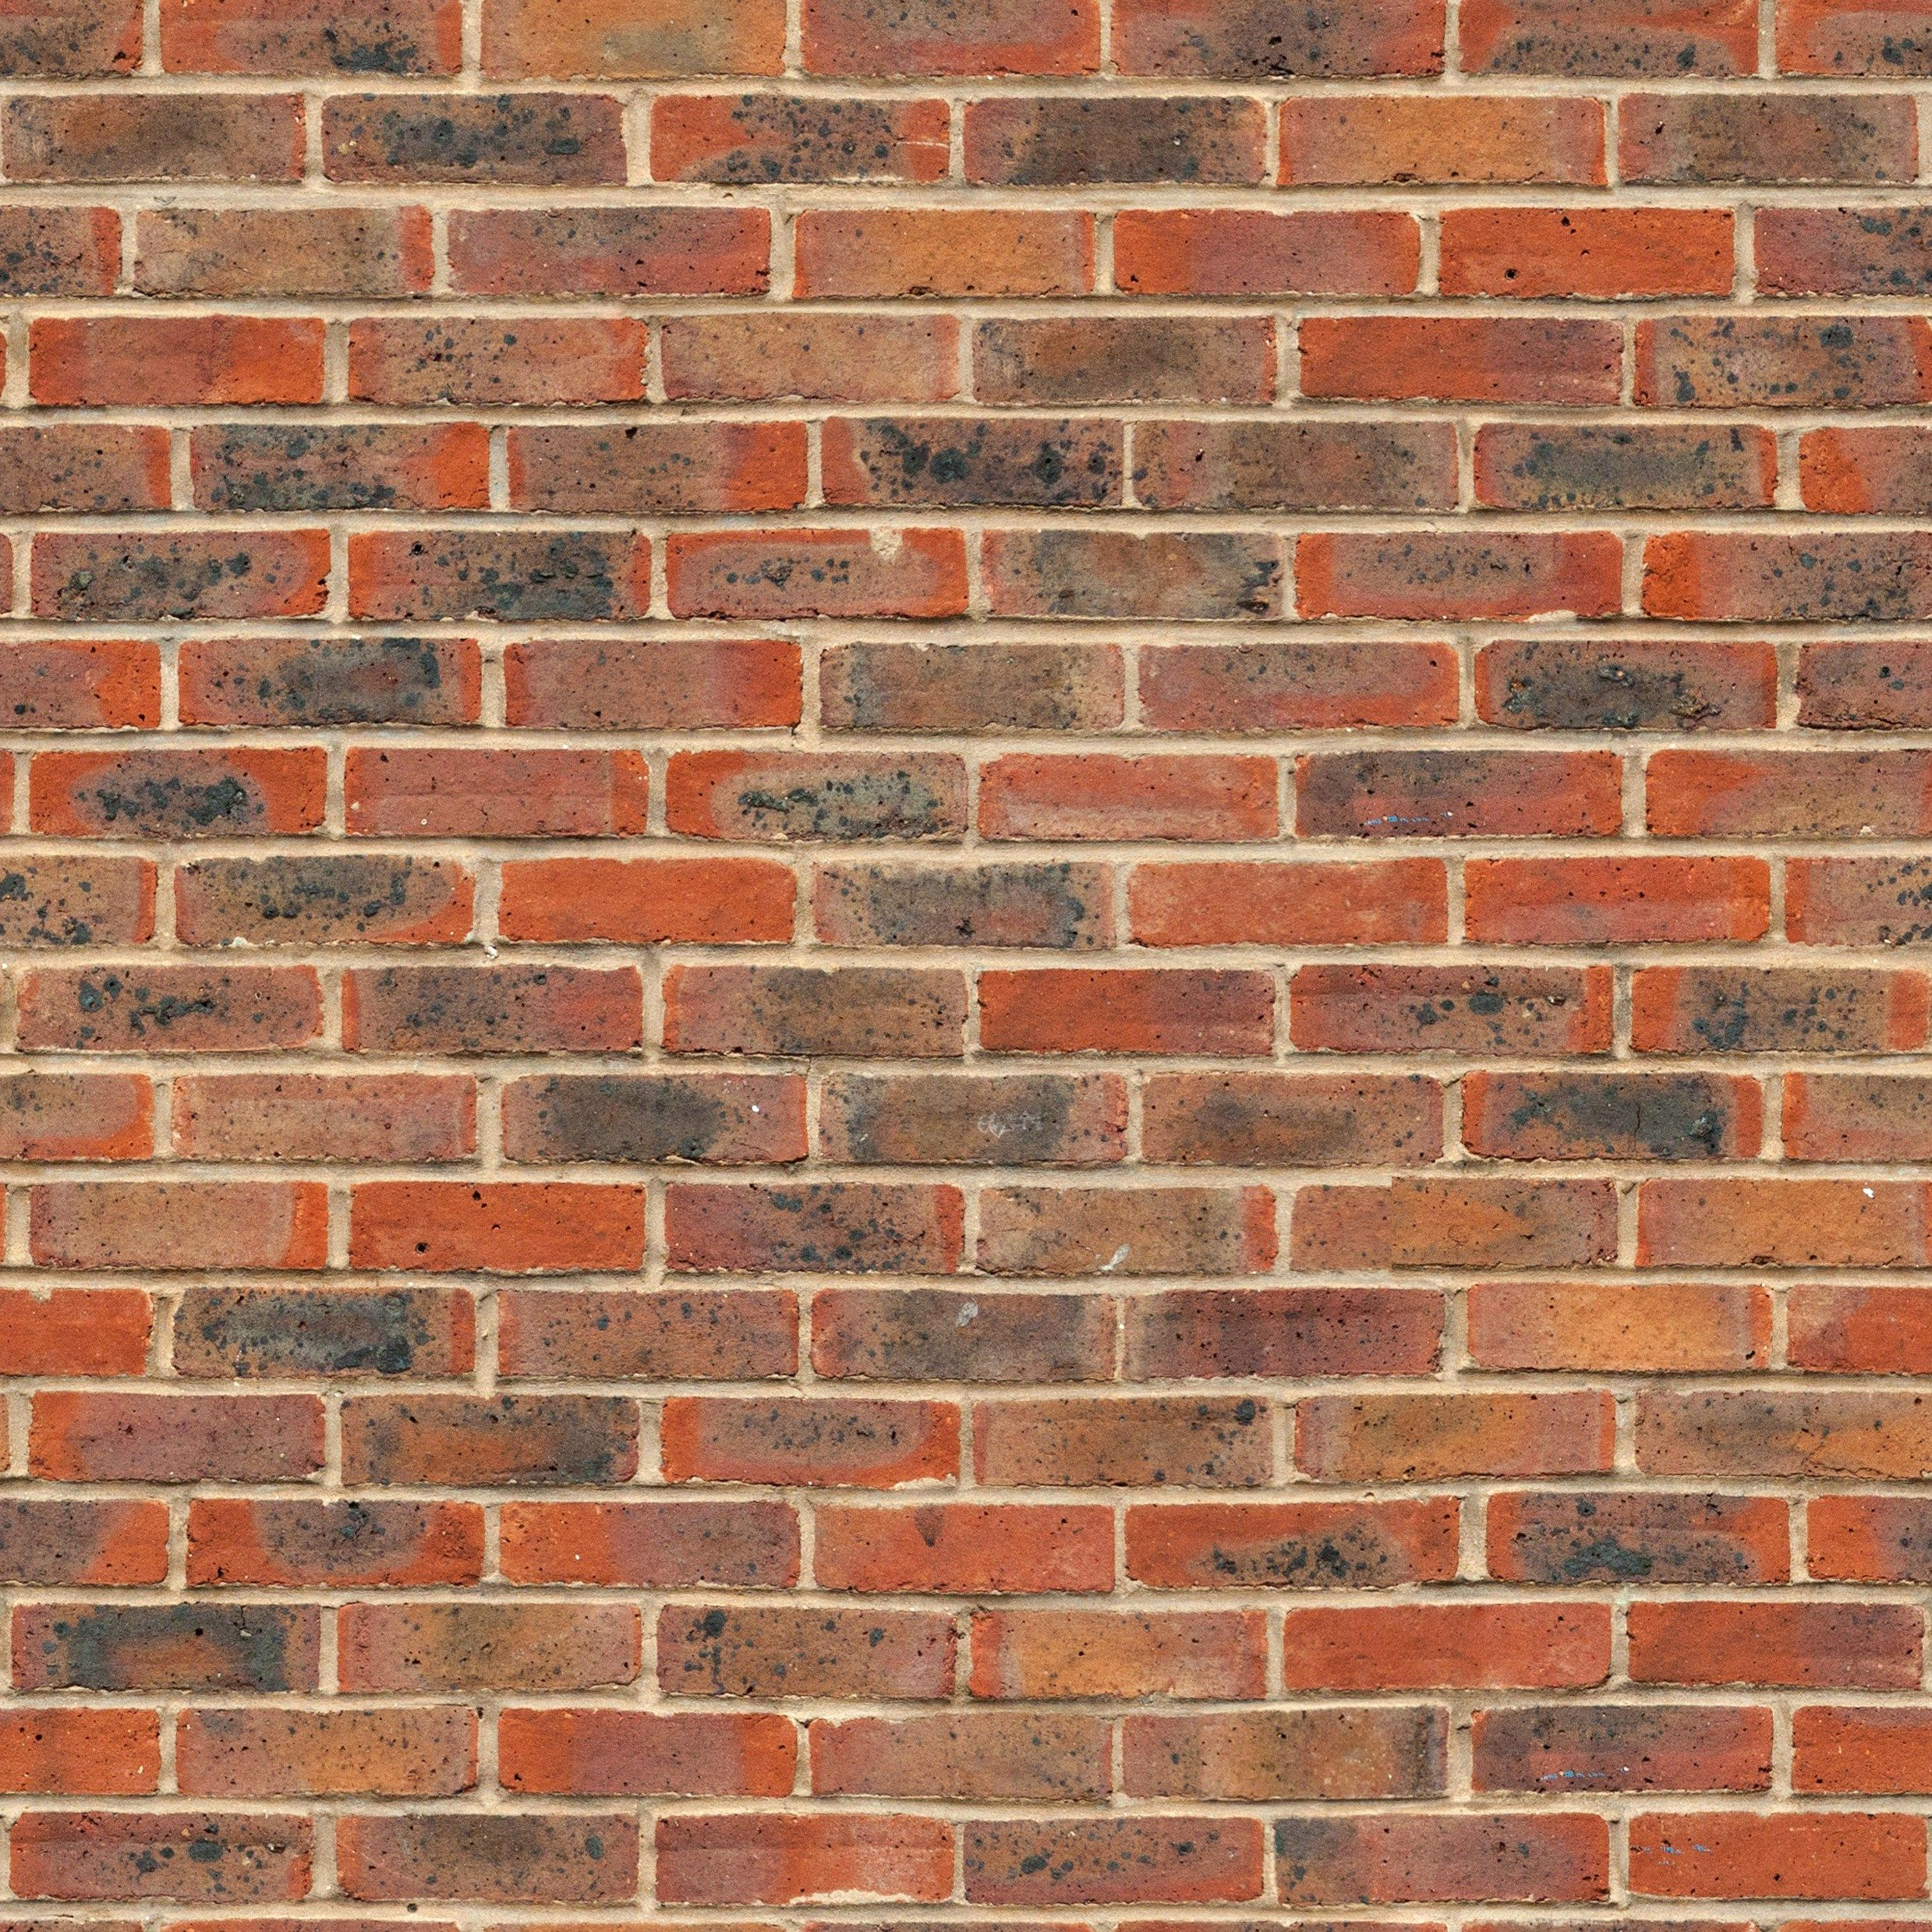
\includegraphics[width=\linewidth]{img/evaluation/adv_brick_real_life_target.jpg}
    \caption{Real life target texture (photograph) $T_{33}$ of a brick wall.}
    \label{fig:TargetM3T33RealLife}
\end{subfigure}
\caption{The three test target textures for shader model $M_3$ including an additional real life target.}
\label{fig:TargetsM3}
\end{figure}

\section{Python Rendering Performance}

The rendering time of our Python shaders can be a major bottleneck during parameter estimation as one texture image is rendered per iteration of gradient descent. The rendering performance is therefore evaluated on the three shaders models described in section \ref{sec:ShaderModelsForEvaluation} for a number of sizes. We use $150$ linearly sampled sizes between $10\times10$ and $1000\times1000$ pixels plus an additional selected size of $200\times200$ which is the default render size in \dipter{}. For each shader and render size, a texture is rendered three times and the average CPU execution time is recorded. The results are plotted in Figure \ref{fig:PythonRenderingPerformance} on a log-log plot where the y-axis shows the rendering time in milliseconds while the number of pixels is displayed on the x-axis. A dotted horizontal line shows the threshold for real time performance, here defined as rendering 30 times per second or more, equivalent to a rendering time of approximately 33ms, and a dotted vertical line marks the default rendering size of $200\times 200$ pixels.

\begin{figure}[h]
    \centering
    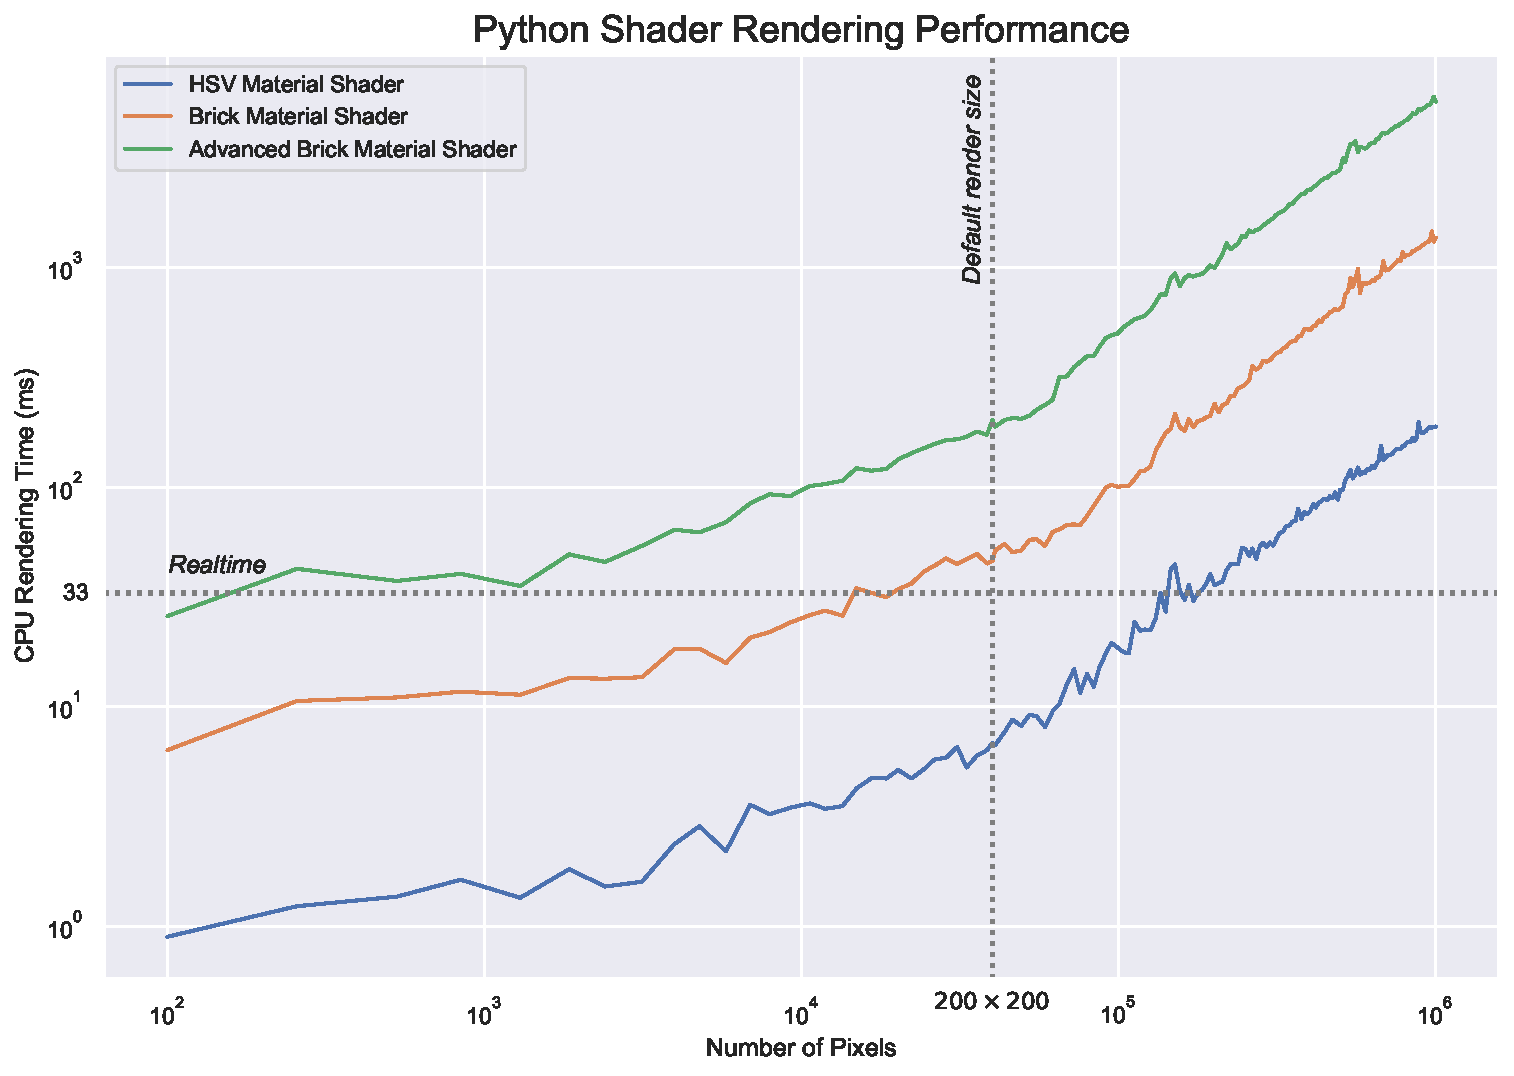
\includegraphics[width=0.9\textwidth]{img/evaluation/PythonRenderingPerformance.pdf}
    \caption{The CPU rendering time in milliseconds it takes to render an image of a certain size, measured in milliseconds per total number of pixels, for the back-end Python render engine. A horizontal dotted line indicates the threshold for real time performance ($33$ms/render) and a vertical dotted line indicates the number of pixels in the default render size ($200\times 200$ pixels).}
    \label{fig:PythonRenderingPerformance}
\end{figure}

We can observe that the rendering time scales linearly with the number of rendered pixels which is expected. Furthermore, rendering performance is largely dictated by the complexity of the shader function. For $M_1$, rendering a texture of default size, $200\times 200$, only takes around 7 milliseconds and we can achieve real time performance for up to a resolution of about $360\times 360$ pixels. For $M_2$, rendering a texture of default size takes considerably longer at about 46 milliseconds and we can only achieve real time performance for textures of up to around $116\times 116$ pixels. Lastly, for the most advanced shader function real time performance is already surpassed at a resolution of $16\times 16$ pixels and rendering a texture using the default resolution takes around 200 milliseconds. While real time performance is by no means a requirement for the Python shading, it will directly affect the time it takes to perform the parameter estimation, as seen in section \ref{sec:EvalParameterEstimation}. A constant part of the total rendering time does not directly depend on the resolution or the number of functions used, but on the number of nodes in the node graph as well as the number of inputs that have to be checked for those nodes. For $M_1$, this is about 1.5 milliseconds, for $M_2$ about 6 milliseconds and for $M_3$ about 20 milliseconds or on average about 1.8 milliseconds per node. 

\section{Parameter Estimation}\label{sec:EvalParameterEstimation}

The algorithm itself used for parameter estimation is fairly simple but needs to solve two difficult problems. First of all, we need a reliable way of finding a path towards a minimum of our loss function and unfortunately there is no way of knowing if the reached minimum is actually a global minimum or a local minimum. Second, the loss functions global minima must correspond to a satisfactory similarity between the target and generated texture, and should ideally be as smooth as possible in all dimensions. In this section, we will therefore survey different optimizer strategies, which solve the first problem, and different loss functions, pertaining to the second problem, for our three test shaders and discuss the advantages and disadvantages of the different combinations.

We rendered a texture from each of our three test shaders where only two variables have been changed, $T_{i1}$, which allows us to plot the loss as a surface dependent on these two variables and trace the parameter estimation progress along this surface. It also serves as an easy starting point of evaluation as we later evaluate parameter estimation using every variable, targets $T_{i2}$.

Evaluating the parameter estimation is done separately for each of the test shader models $M_1$, $M_2$ and $M_3$ for each possible combination of our three implemented loss functions, see section \ref{sec:MethodLossFunctions}, and optimizers. The optimizers we chose to test are the popular \textit{Adam} and the predecessor \textit{RMSprop}, both of which comes bundled with PyTorch. When performing the gradient descent, the initial state of the shader model is equivalent to that shown in the node setups in figures \ref{fig:M1NodeGraphAndDefaultRender}, \ref{fig:M2NodeGraphAndDefaultRender} and \ref{fig:M3NodeGraphAndDefaultRender} respectively. Normally when gradient descent is used to optimize a neural network the initial parameters are randomized, which is not best practice in \dipter{} as a user will typically design their shader model as far as possible and then use the parameter estimation as a final step to find even better parameter values. Randomizing initial parameters will effectively undo all of the user's progress and will in most cases result in a higher initial loss. All textures are compared as matrices where the color values are stored as floating point values ranging from $0.0$ to $1.0$. All plots follow the convention that parameter estimations for $T_{i1}$ are shown as solid lines while parameter estimations for the $T_{i2}$ targets are shown as dotted lines, additionally using blue or orange color when using Adam or RMSprop, respectively.

\subsection{Parameter Estimation Speed}\label{sec:EvalParameterEstimationSpeed}

Difficult optimization problems often require hundreds of iterations to reach a low loss value and the execution time of a loss function can thus greatly influence the overall parameter estimation time. In Figure \ref{fig:ParameterEstimationSpeed} the average iteration time per shader per loss function is presented. This data was produced by executing 10 iterations of gradient descent three times with both Adam and RMSprop and then averaging over those times. We did not separate the data between the different optimizers as there was no significant difference between them. The rendering resolution was set to $224\times224$ pixels, the required resolution of input to VGG19 used in the neural loss function, and the rendering time is included in the plot. It is clear that Mean Squared Error and Squared Bin Loss are much faster functions than the Neural Loss and the almost constant difference between their execution time suggests that the total time mainly scales with the render resolution and complexity of shader model. In cases where a neural loss function does not clearly result in a more accurate result, there is not much justification for its greater execution time. However, when the model is sufficiently complex so that the rendering time is the largest factor, in terms of iteration time, it does not matter much which loss function is used. 

\begin{figure}
    \centering
    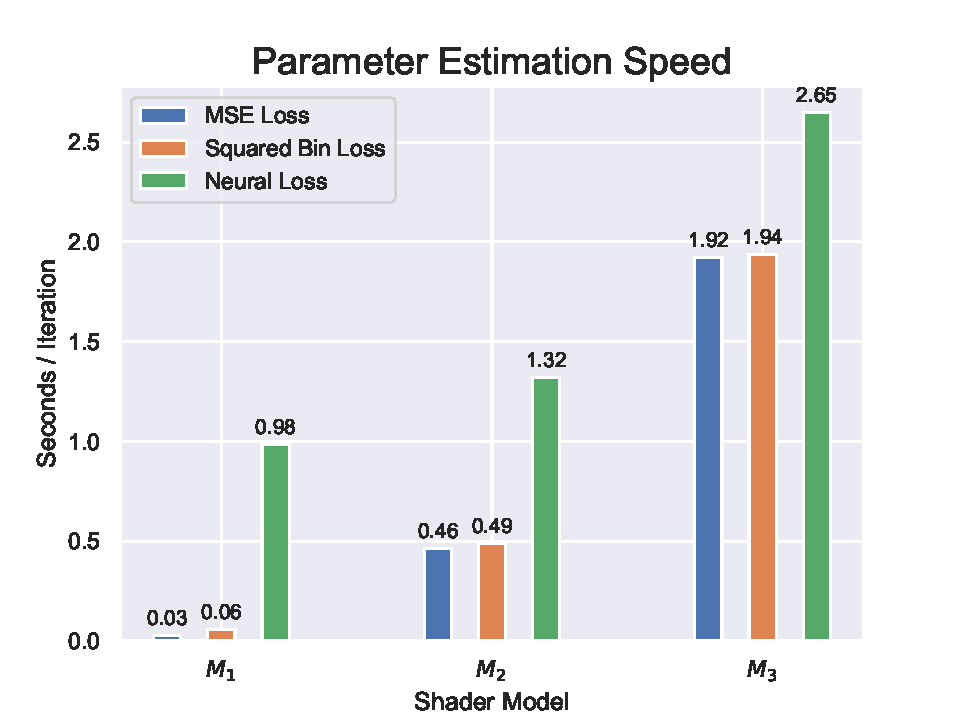
\includegraphics[width=0.9\textwidth]{img/evaluation/Parameter Estimation Speed.pdf}
    \caption{Execution time in seconds for an iteration of gradient descent for different shader models and loss functions. The iteration time includes the process of rendering an image from the shader model once using a resolution of $224\times224$ pixels.}
    \label{fig:ParameterEstimationSpeed}
\end{figure}


\subsection{Parameter Estimation using MSE}

\begin{table}[h]
\centering
\begin{tabular}{ccllllll}
\textbf{}      &                   & \textbf{}          & \multicolumn{1}{l|}{}            & \multicolumn{2}{l|}{\textit{Adam}}                           & \multicolumn{2}{l|}{\textit{RMSprop}}                      \\
\textbf{$M_i$} & \textbf{$T_{ij}$} & \textbf{Optimizer} & \multicolumn{1}{l|}{\textbf{lr}} & \textbf{$\beta_1$} & \multicolumn{1}{l|}{\textbf{$\beta_2$}} & \textbf{$\alpha$} & \multicolumn{1}{l|}{\textbf{Momentum}} \\ \hline
 $M_1$      & $T_{11}$   & Adam       & 0.15       & 0.5        & 0.999      &            &           \\
 $M_1$      & $T_{11}$   & RMSprop    & 0.09       &            &            & 0.9        & 0.0       \\
 $M_1$      & $T_{12}$   & Adam       & 0.1        & 0.5        & 0.999      &            &           \\
 $M_1$      & $T_{12}$   & RMSprop    & 0.09       &            &            & 0.9        & 0.0       \\
 $M_2$      & $T_{21}$   & Adam       & 0.05       & 0.9        & 0.999      &            &           \\
 $M_2$      & $T_{21}$   & RMSprop    & 0.01       &            &            & 0.75       & 0.4       \\
 $M_2$      & $T_{22}$   & Adam       & 0.05       & 0.8        & 0.999      &            &           \\
 $M_2$      & $T_{22}$   & RMSprop    & 0.02       &            &            & 0.75       & 0.6       \\
 $M_3$     & $T_{31}$   & Adam       & 0.05       & 0.9        & 0.999      &            &            \\
 $M_3$     & $T_{31}$   & RMSprop    & 0.01       &            &            & 0.75       & 0.4        \\
 $M_3$     & $T_{32}$   & Adam       & 0.05       & 0.8        & 0.999      &            &            \\
 $M_3$     & $T_{32}$   & RMSprop    & 0.02       &            &            & 0.75       & 0.6        \\
 $M_3$     & $T_{33}$   & Adam       & 0.04       & 0.9        & 0.999      &            &            \\
 $M_3$     & $T_{33}$   & RMSprop    & 0.01       &            &            & 0.75       & 0.4        \\
\end{tabular}
\caption{Optimizer and loss function settings when running gradient descent using Mean Squared Error loss.}
\label{tab:MSEOptimizerSettings}
\end{table}

Mean Squared Error is a loss function that measures the difference in color values for each channel and pixel between our generated image $\hat{X}$ and target $X$. \hl{It is a very simple loss function and is such much faster than, for example, a neural loss function and is well suited for} finding the similarity between simple textures without patterns as it heavily depends on spatial information. The minimum loss value that can be achieved is $0.0$ corresponding to an exact match in color values and the maximum loss is $1.0$ corresponding to a maximum difference between each pixel which stems from our use of a floating point image format. The settings used for each shader model and optimizer when evaluating Mean Squared Error loss is presented in table \ref{tab:MSEOptimizerSettings}. Each optimizer and target requires different settings to perform well and typically, a more difficult problem requires a lower learning rate and more iterations to optimize successfully.

\subsubsection{HSV Test Shader $M_1$}

\begin{figure}[ht]
    \centering
    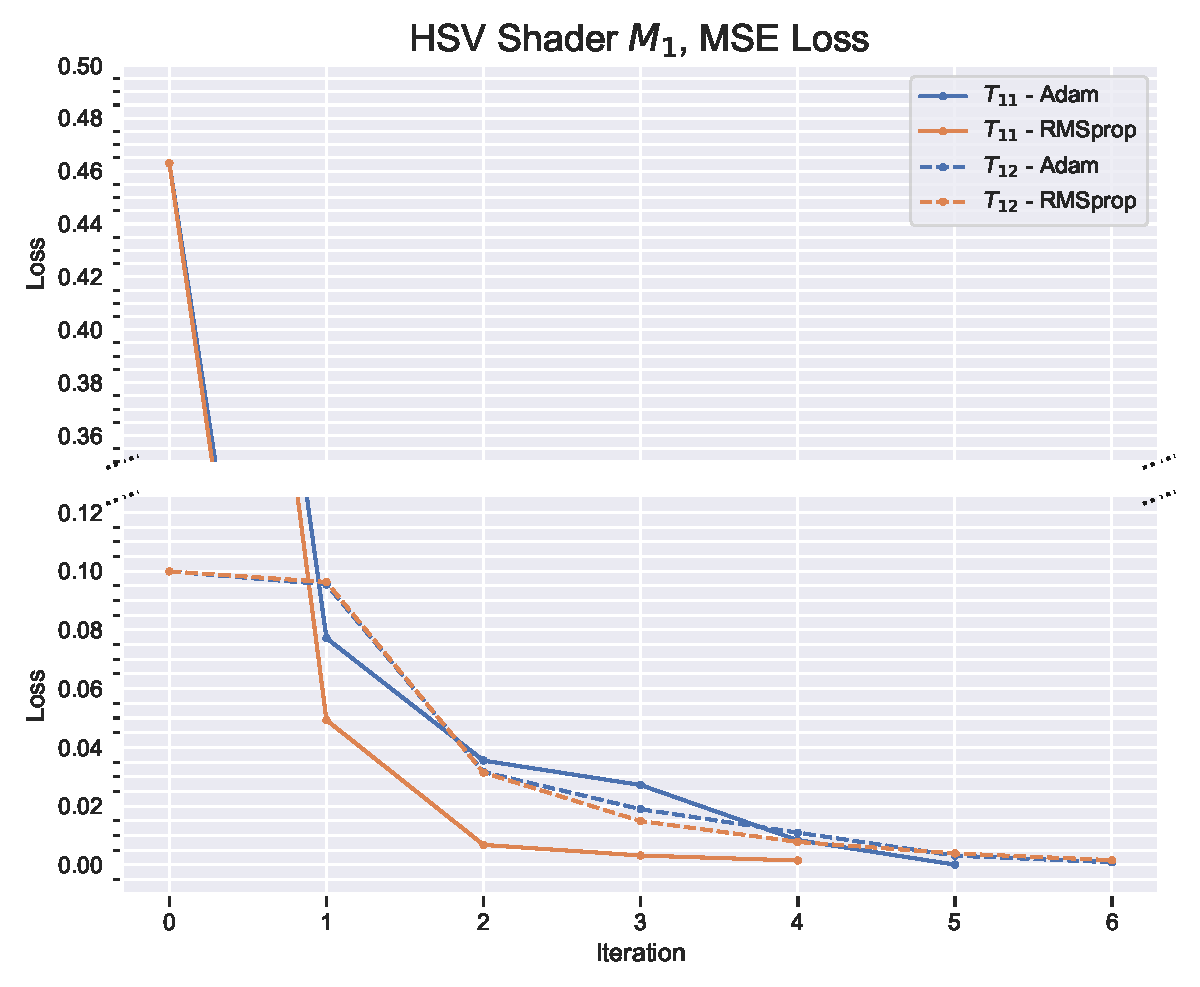
\includegraphics[width=0.8\textwidth]{img/evaluation/M1/HSV_MSE.pdf}
    \caption{Results of evaluating parameter estimation of material $M_1$ using Mean Squared Error loss. The runs with target $T_{11}$ are plotted as solid lines while runs with target $T_{12}$ are plotted with dashed lines.}
    \label{fig:M1MSEData}
\end{figure}

First, parameter estimation using an MSE loss function with $M_1$ is evaluated and the results are shown in Figure \ref{fig:M1MSEData}. The target loss threshold is set to $0.0025$ corresponding to an average difference in color values of $\sqrt{0.0025}=0.05$ or $5\%$. We are able to reach the loss threshold in only a few iterations using either optimization methods. As expected, a few more iterations are required to reach the threshold for target $T_{12}$ as more parameters have to be optimized, even though the initial loss is actually lower than for $T_{11}$. Furthermore, a simple model like $M_1$ seems to be more efficiently optimized using RMSprop than the more modern Adam, possibly due to Adam requiring a few initial iterations in order to build up momentum. For this experiment, using a learning rate of under $1.0$ proved a necessity for RMSprop, where using a larger value resulted in a divergence of the loss. Lowering the first moment parameter $\beta_1$ for Adam proved very helpful in order to diminish its oscillating behaviour. Typically, MSE is not a very good loss function for image comparison, but as $M_1$ is uniform across the entire image, the spatial dependence of MSE is not a problem and proves very efficient for similar problems.

\subsubsection{Simple Brick Test Shader $M_2$}
\begin{figure}[hp]
    \centering
    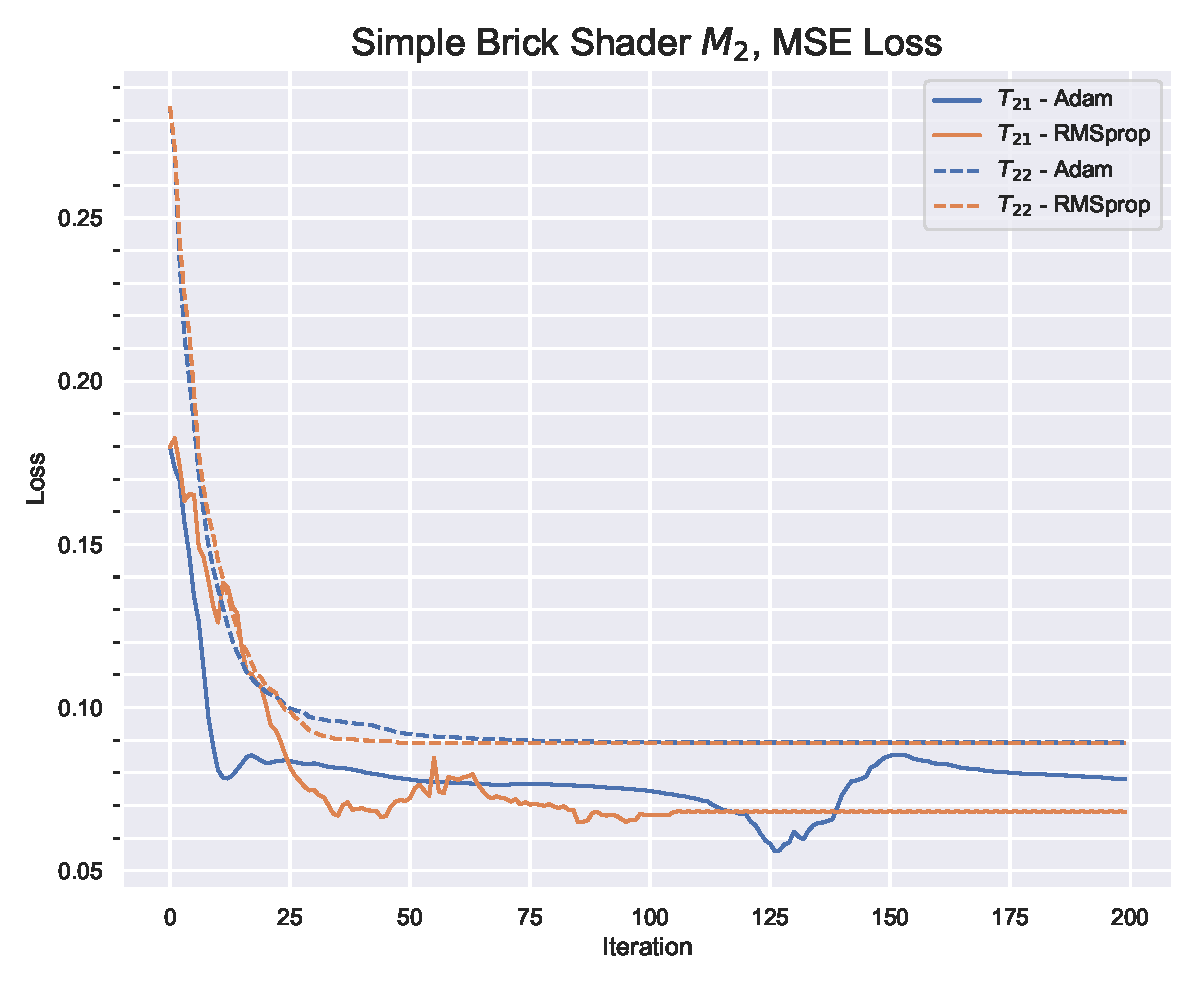
\includegraphics[width=0.8\textwidth]{img/evaluation/M2/SBS_MSE.pdf}
    \caption{Results of evaluating parameter estimation of material $M_2$ using Mean Squared Error loss. The runs with target $T_{21}$ are plotted as solid lines while runs with target $T_{22}$ are plotted with dashed lines.}
    \label{fig:M2MSEData}
\end{figure}

\begin{figure}[hp]
\centering
\begin{subfigure}[t]{.25\textwidth}
    \centering
    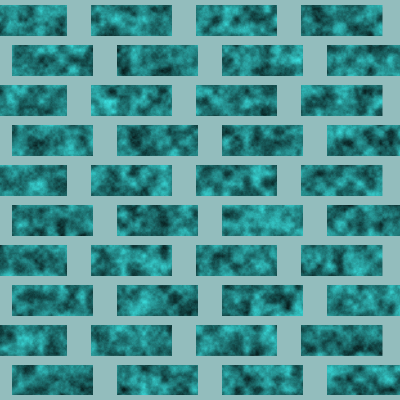
\includegraphics[width=\linewidth]{img/evaluation/M2/2param/MSE_Adam_final_render.png}
    \caption{Target $T_{21}$ using Adam.}
    \label{fig:M2MSEFinalRenders2paramAdam}
\end{subfigure}\hspace{0.7cm}
\begin{subfigure}[t]{.25\textwidth}
    \centering
    
\includegraphics[width=\linewidth]{img/evaluation/M2/random/MSE_Adam_random_final_render.png}
    \caption{Target $T_{22}$ using Adam.}
    \label{fig:M2MSEFinalRendersRandomAdam}
\end{subfigure}
\vskip\baselineskip
\begin{subfigure}[t]{.25\textwidth}
    \centering
    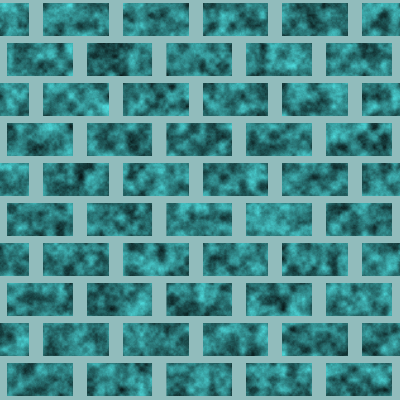
\includegraphics[width=\linewidth]{img/evaluation/M2/2param/MSE_RMSprop_final_render.png}
    \caption{Target $T_{21}$ using RMSprop.}
    \label{fig:M2MSEFinalRenders2paramRMSprop}
\end{subfigure}\hspace{0.7cm}
\begin{subfigure}[t]{.25\textwidth}
    \centering
    
\includegraphics[width=\linewidth]{img/evaluation/M2/random/MSE_RMSprop_random_final_render.png}
    \caption{Target $T_{22}$ using RMSprop.}
    \label{fig:M2MSEFinalRendersRandomRMSprop}
\end{subfigure}
\caption{The four rendered textures at the point of minimal loss for $M_2$ using MSE loss corresponding to the four plots in Figure \ref{fig:M2MSEData} with combinations of optimizers Adam or RMSprop and targets $T_{21}$ or $T_{22}$.}
\label{fig:M2MSEFinalRenders}
\end{figure}

Next, we use the MSE loss function to estimate parameters for the more complex brick shader model $M_2$. Unlike $M_1$ this model is not uniform accross the image and features lots of patterns and even pseudorandom noise which MSE is very ill equipped to handle. Looking at the resulting data in Figure \ref{fig:M2MSEData} we can see that for target $T_{21}$ we are able to find a parameter set that significantly lowers the loss value from around $0.18$ down to a minimum of $0.056$ at iteration 126 for Adam and $0.065$ for RMSprop significantly earlier at iteration 85. In all four cases we lowered the learning rate compared to $M_1$ as this is a more difficult problem with more parameters, as well as increased the $\beta_1$ value to $0.9$ in order to stabilize the progress. Momentum was also utilized here for RMSprop which seemed to help with finding a slightly better minimum. As stated before, MSE is not a good choice for images with patterns but can be efficient at finding the overall color tone of the image. For both optimizers for target $T_{21}$ the blue color of the bricks are successfully reproduced, but not the brick shape, even though Adam managed to produce a result with slightly elongated bricks. As expected, the optimization for target $T_{22}$ was not as successful and did only reach a minimum loss of about $0.089$ for both optimizers which converged around iteration 75. The final renders with the optimized parameters are shown in Figure \ref{fig:M2MSEFinalRenders}. For a relatively complex shader like $M_2$ it seems to be only possible to reproduce the overall color tone of the target texture, but any pattern is either completely lost as in renders \ref{fig:M2MSEFinalRendersRandomAdam} and \ref{fig:M2MSEFinalRendersRandomRMSprop} or the shape is not correctly recovered as in renders \ref{fig:M2MSEFinalRenders2paramAdam} and \ref{fig:M2MSEFinalRenders2paramRMSprop}.

\subsubsection{Advanced Brick Test Shader $M_3$}
\begin{figure}[hp]
    \centering
    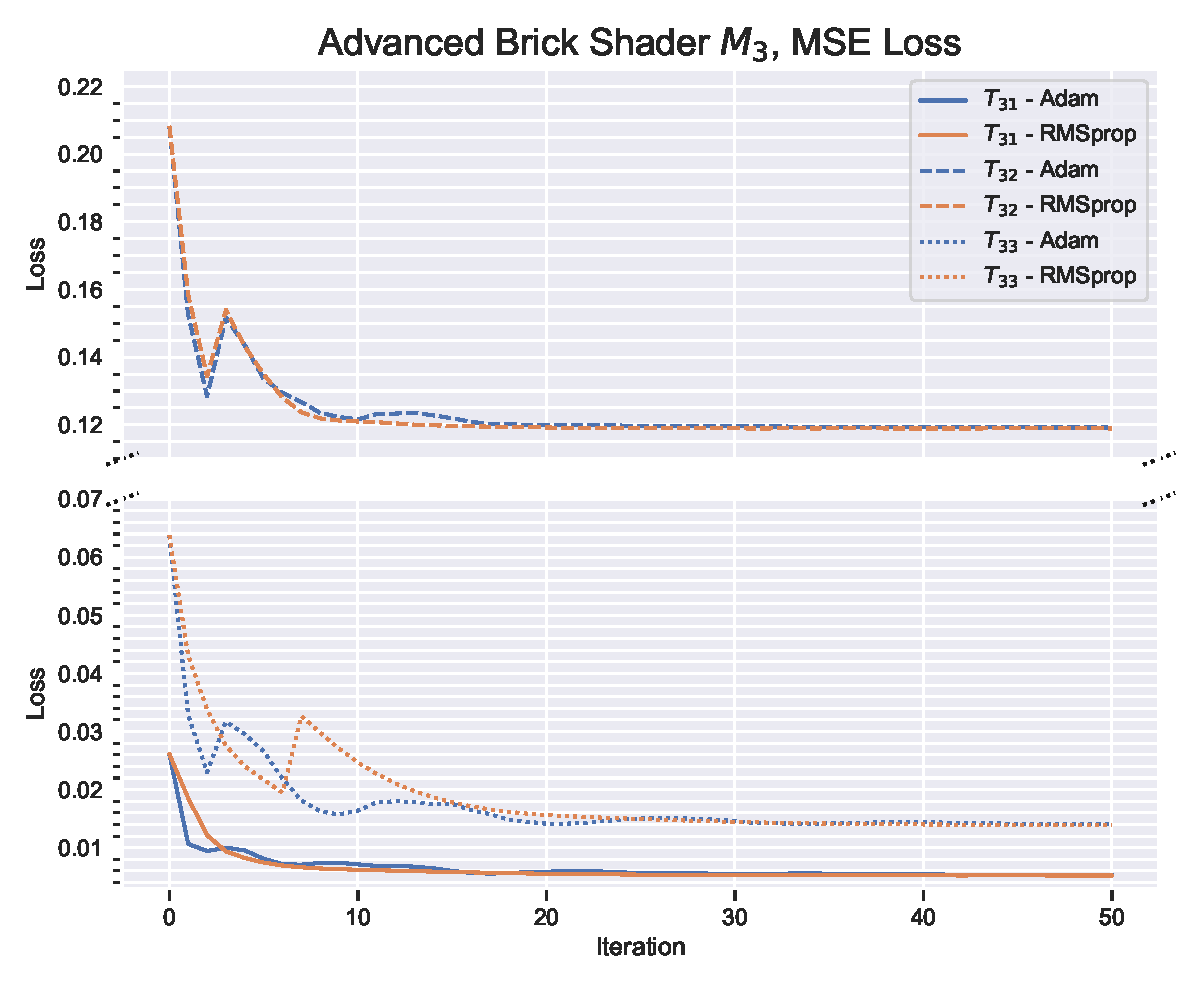
\includegraphics[width=0.8\textwidth]{img/evaluation/M3/ABS_MSE.pdf}
    \caption{Results of evaluating parameter estimation of material $M_3$ using Mean Squared Error loss. The runs with target $T_{31}$ are plotted as solid lines, target $T_{32}$ with dashed lines and the additional real-life target $T_{33}$ with dotted lines. The iterations have been truncated from 200 to 50 iterations as the loss converges before iteration 50.}
    \label{fig:M3MSEData}
\end{figure}

Finally test shader $M_3$ is evaluated using the MSE loss function and the results are shown in Figure \ref{fig:M3MSEData} and best renders in Figure \ref{fig:M3MSEFinalRenders} where the same optimizer settings were used as with $M_2$ for targets $T_{31}$ and $T_{32}$. For target $T_{31}$, the initial loss is relatively low at just above $0.025$ and both optimizers reaches a minimum loss of $0.0052$, fairly close to our threshold of $0.0025$. This demonstrates the fact that MSE often does not correspond with how humans judge similarity, because when comparing the initial render in \ref{fig:M3NodeGraphAndDefaultRender} and the target $T_{31}$ in \ref{fig:TargetM3T31TwoParam} they clearly portray very different brick walls. The optimization looks rather successful on paper, but looking at the render from the parameters at the point of minimal loss in Figure \ref{fig:M3MSEFinalRenders}, only the average color has been captured. As expected, the performance for target $T_{32}$ using random parameters is worse, only reaching a minimum loss of about $0.12$ around iteration 20 for either optimizer. The additional real-life target $T_{33}$ plotted with dotted lines lies somewhere in between, starting with a loss of about $0.065$ and converging to a loss of about $0.014$. The same behaviour is shown here as seen before, where the renders in sub-figures \ref{fig:M3MSEFinalRendersRealLifeAdam} and \ref{fig:M3MSEFinalRendersRealLifeRMSprop} show that the MSE loss only restores the overall color of the target. Clearly a Mean Squared Error loss is not optimal when estimating parameters for complex shaders with an extensive use of patterns.  
\begin{figure}[h]
\centering
\begin{subfigure}[t]{.25\textwidth}
    \centering
    
\includegraphics[width=\linewidth]{img/evaluation/M3/2 param/MSE_Adam_2_param_final.png}
    \caption{Target $T_{31}$ using Adam.}
    \label{fig:M3MSEFinalRendersTwoParamAdam}
\end{subfigure}\hspace{0.7cm}
\begin{subfigure}[t]{.25\textwidth}
    \centering
    
\includegraphics[width=\linewidth]{img/evaluation/M3/random/MSE_Adam_random_final.png}
    \caption{Target $T_{32}$ using Adam.}
    \label{fig:M3MSEFinalRendersRandomAdam}
\end{subfigure}\hspace{0.7cm}
\begin{subfigure}[t]{.25\textwidth}
    \centering
    
\includegraphics[width=\linewidth]{img/evaluation/M3/real life/MSE_Adam_real_life_final.png}
    \caption{Target $T_{33}$ using Adam.}
    \label{fig:M3MSEFinalRendersRealLifeAdam}
\end{subfigure}
\vskip\baselineskip
\begin{subfigure}[t]{.25\textwidth}
    \centering
    
\includegraphics[width=\linewidth]{img/evaluation/M3/2 param/MSE_RMSprop_2_param_final.png}
    \caption{Target $T_{31}$ using RMSprop.}
    \label{fig:M3MSEFinalRendersTwoParamRMSprop}
\end{subfigure}\hspace{0.7cm}
\begin{subfigure}[t]{.25\textwidth}
    \centering
    
\includegraphics[width=\linewidth]{img/evaluation/M3/random/MSE_RMSprop_random_final.png}
    \caption{Target $T_{32}$ using RMSprop.}
    \label{fig:M3MSEFinalRendersRandomRMSprop}
\end{subfigure}\hspace{0.7cm}
\begin{subfigure}[t]{.25\textwidth}
    \centering
    
\includegraphics[width=\linewidth]{img/evaluation/M3/real life/MSE_RMSprop_real_life_final.png}
    \caption{Target $T_{33}$ using RMSprop.}
    \label{fig:M3MSEFinalRendersRealLifeRMSprop}
\end{subfigure}
\caption{The six rendered textures at the point of minimal loss for $M_3$ using an MSE loss function corresponding to the six plots in Figure \ref{fig:M3MSEData} with combinations of optimizers Adam or RMSprop and targets $T_{31}$, $T_{32}$ or $T_{33}$.}
\label{fig:M3MSEFinalRenders}
\end{figure}

\subsection{Parameter Estimation using Squared Bin Loss}

\begin{table}[h]
\centering
\begin{tabular}{cclllllll}
\textbf{}      &                   & \textbf{}          & \multicolumn{1}{l|}{}            & \multicolumn{2}{l|}{\textit{Adam}}                           & \multicolumn{2}{l|}{\textit{RMSprop}}                      & \multicolumn{1}{l|}{\textit{SBL}}      \\
\textbf{$M_i$} & \textbf{$T_{ij}$} & \textbf{Optimizer} & \multicolumn{1}{l|}{\textbf{lr}} & \textbf{$\beta_1$} & \multicolumn{1}{l|}{\textbf{$\beta_2$}} & \textbf{$\alpha$} & \multicolumn{1}{l|}{\textbf{Momentum}} & \multicolumn{1}{l|}{\textbf{Bin Size}} \\ \hline
 $M_1$      & $T_{11}$   & Adam       & 0.15       & 0.5        & 0.999      &            &            & 10        \\
 $M_1$      & $T_{11}$   & RMSprop    & 0.09       &            &            & 0.9        & 0.0        & 10        \\
 $M_1$      & $T_{12}$   & Adam       & 0.1        & 0.5        & 0.999      &            &            & 10        \\
 $M_1$      & $T_{12}$   & RMSprop    & 0.09       &            &            & 0.9        & 0.0        & 10        \\
 $M_2$     & $T_{21}$   & Adam       & 0.03       & 0.8        & 0.999      &            &            & 8          \\
 $M_2$     & $T_{21}$   & RMSprop    & 0.02       &            &            & 0.9        & 0.4        & 8          \\
 $M_2$     & $T_{22}$   & Adam       & 0.03       & 0.8        & 0.999      &            &            & 8          \\
 $M_2$     & $T_{22}$   & RMSprop    & 0.02       &            &            & 0.9        & 0.4        & 8          \\
  $M_3$     & $T_{31}$   & Adam       & 0.03       & 0.8        & 0.999      &            &            & 8          \\
 $M_3$     & $T_{31}$   & RMSprop    & 0.015      &            &            & 0.99       & 0.4        & 8          \\
 $M_3$     & $T_{32}$   & Adam       & 0.03       & 0.8        & 0.999      &            &            & 8          \\
 $M_3$     & $T_{32}$   & RMSprop    & 0.01       &            &            & 0.99       & 0.2        & 8          \\
\end{tabular}
\caption{Optimizer and loss settings when running gradient descent using Squared Bin loss.}
\label{tab:SBLOptimizerSettings}
\end{table}

Squared Bin Loss or SBL is effectively a version of Mean Squared Error that first downscales images into squared bins of a user controllable size and calculates the mean of each bin before returning the Mean Squared Error of the averages. This allows the loss function to better judge image similarity without comparing every pixel individually and can for some types of images help discern underlying patterns among noise. The loss value limits are the same as for the MSE loss, a minimum loss of $0.0$ and a maximum loss of $1.0$. Unlike MSE however, a loss value of $0.0$ for SBL does not necessarily mean that the images are identical, simply that the average of each bin is identical. The optimizer settings used when running gradient descent for SBL is presented in table \ref{tab:SBLOptimizerSettings}.

\newpage
\subsubsection{HSV Test Shader $M_1$}

\begin{figure}[hpt]
    \centering
    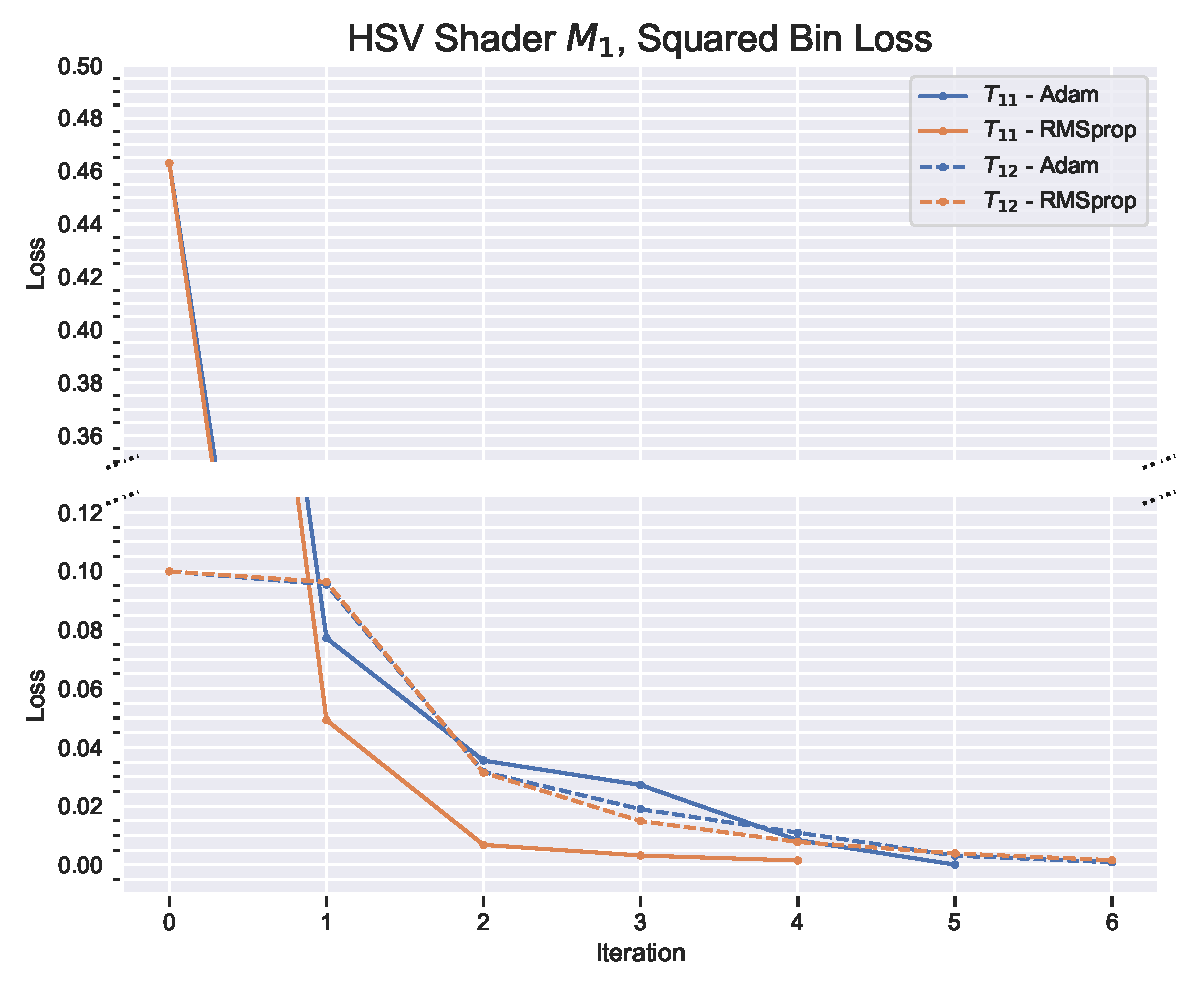
\includegraphics[width=0.8\textwidth]{img/evaluation/M1/HSV_SBL.pdf}
    \caption{Results of evaluating parameter estimation of material $M_1$ using Squared Bin loss. The runs with target $T_{11}$ are plotted as solid lines while runs with target $T_{12}$ are plotted with dashed lines.}
    \label{fig:M1SBLData}
\end{figure}

For uniform textures like those produced by $M_1$, SBL should give exactly the same result as a normal MSE loss, which is why it is curious that the loss threshold is reached, on average, one iteration earlier for SBL than MSE as shown in Figure \ref{fig:M1SBLData}, even if the exact same optimizer settings are used. This is probably more or less the result of chance, as the gradients are affected by the additional PyTorch functions used and so even if the same loss value is returned for the same data, the gradients are slightly different. Generally, this loss works equally well for uniform shaders as MSE and we were able to reach the loss threshold of $0.0025$ for both targets in five or less iterations. Similar to using MSE loss, RMSprop managed to slightly outperform Adam in this simple use case as well.

\subsubsection{Simple Brick Test Shader $M_2$}

\begin{figure}[hpb]
    \centering
    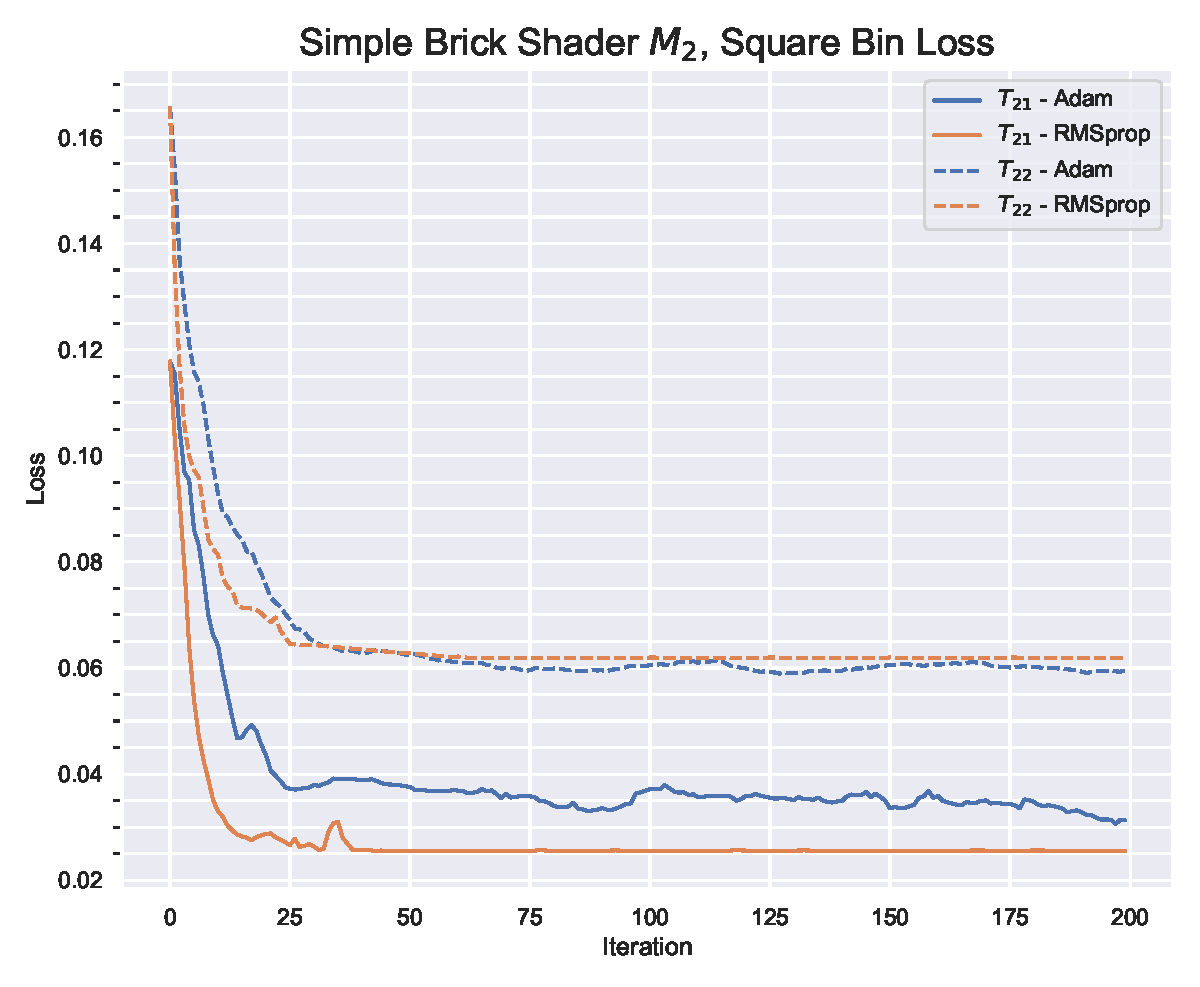
\includegraphics[width=0.8\textwidth]{img/evaluation/M2/SBS_SBL.pdf}
    \caption{Results of evaluating parameter estimation of material $M_2$ using Squared Bin loss. The runs with target $T_{21}$ are plotted as solid lines while runs with target $T_{22}$ are plotted with dashed lines.}
    \label{fig:M2SBLData}
\end{figure}

\begin{figure}[h]
\centering
\begin{subfigure}[t]{.25\textwidth}
    \centering
    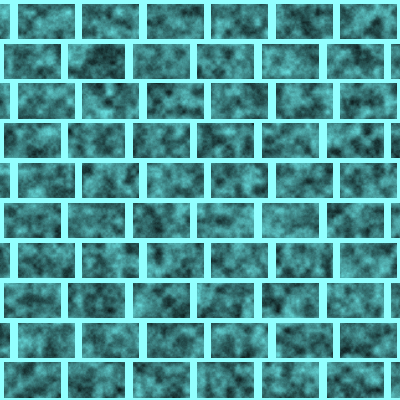
\includegraphics[width=\linewidth]{img/evaluation/M2/2param/SBL_Adam_two_param_final.png}
    \caption{Target $T_{21}$ using Adam.}
    \label{fig:M2SBLFinalRenders2paramAdam}
\end{subfigure}\hspace{0.5cm}
\begin{subfigure}[t]{.25\textwidth}
    \centering
    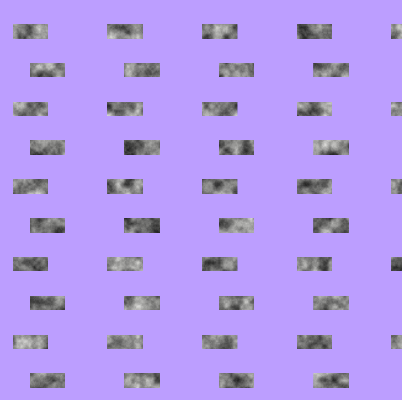
\includegraphics[width=\linewidth]{img/evaluation/M2/random/SBL_Adam_random_final.png}
    \caption{Target $T_{22}$ using Adam.}
    \label{fig:M2SBLFinalRendersRandomAdam}
\end{subfigure}
\vskip\baselineskip
\begin{subfigure}[t]{.25\textwidth}
    \centering
    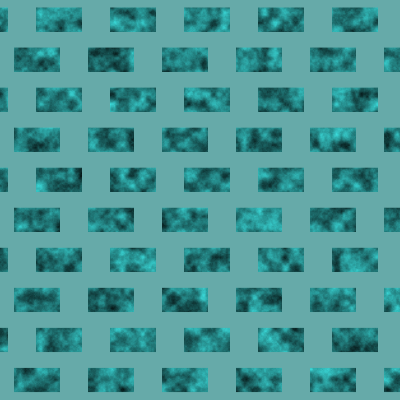
\includegraphics[width=\linewidth]{img/evaluation/M2/2param/SBL_RMSprop_two_param_final.png}
    \caption{Target $T_{21}$ using RMSprop.}
    \label{fig:M2SBLFinalRenders2paramRMSprop}
\end{subfigure}
\hspace{0.5cm}
\begin{subfigure}[t]{.25\textwidth}
    \centering
    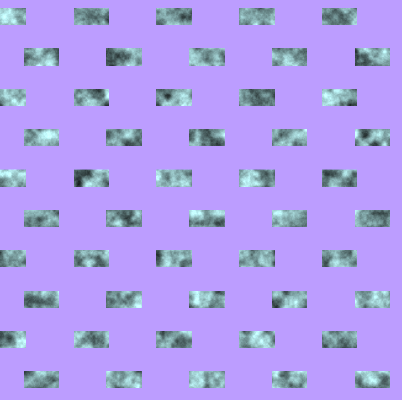
\includegraphics[width=\linewidth]{img/evaluation/M2/random/SBL_RMSprop_random_final.png}
    \caption{Target $T_{22}$ using RMSprop.}
    \label{fig:M2SBLFinalRendersRandomRMSprop}
\end{subfigure}
\caption{The four rendered textures at the point of minimal loss for $M_2$ using SBL corresponding to the six plots in Figure \ref{fig:M2SBLData} with combinations of optimizers Adam or RMSprop and targets $T_{21}$ or $T_{32}$.}
\label{fig:M2SBLFinalRenders}
\end{figure}

For test shader $M_2$ we used much lower learning rates than for $M_1$ and a higher $\beta_1$ for Adam while adding some momentum for RMSprop. The bin size was set to $8$ meaning bins of $8\times 8$ pixels are averaged, as lower values did not contribute to the accuracy and larger values would introduce too much averaging and thereby lose detail. The results are shown in Figure \ref{fig:M2SBLData} where it is apparent that for target $T_{21}$ RMSprop is outperforming Adam by a significant amount. At iteration 45 RMSprop has reached its best loss value of approximately $0.025$ while Adam reaches its best loss value of $0.03$ at iteration 197. For target $T_{22}$ the results are more even, Adam reaching a loss of around $0.059$ at iteration 127 while RMSprop reaches a loss of around $0.062$ at iteration 146. In Figure \ref{fig:M2SBLFinalRenders} we can see that the results are similar to those for MSE; the overall color has been captured, at the expense of the background color, but not the shape of the bricks although the results look slightly better for target $T_{22}$ where the bricks have been conserved but scaled down.

\subsubsection{Advanced Brick Test Shader $M_3$}

\begin{figure}[hp]
    \centering
    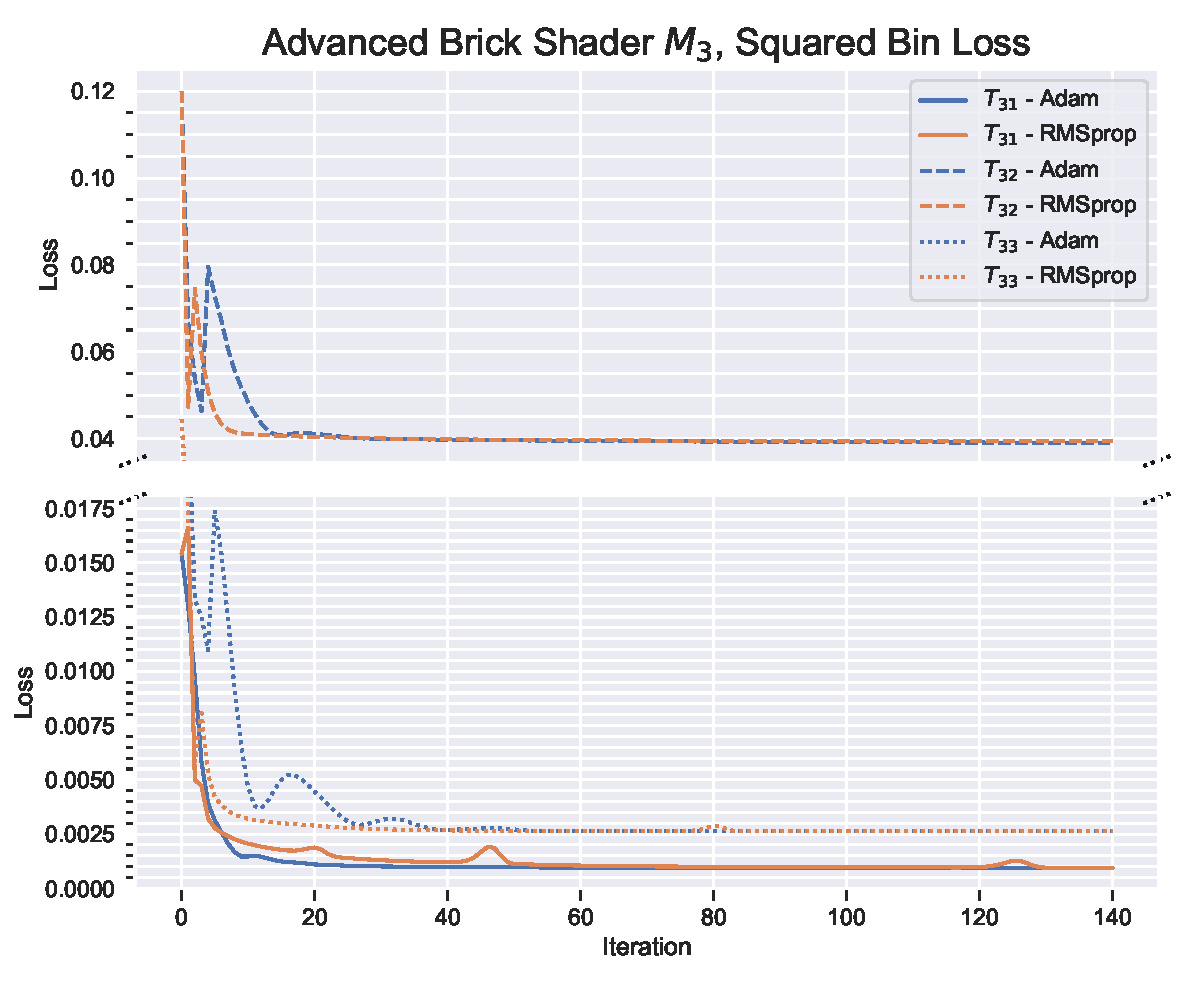
\includegraphics[width=0.8\textwidth]{img/evaluation/M3/ABS_SBL.pdf}
    \caption{Results of evaluating parameter estimation of material $M_3$ using Squared Bin loss. The runs with target $T_{31}$ are plotted as solid lines, target $T_{32}$ with dashed lines and the additional real-life target $T_{33}$ with dotted lines.}
    \label{fig:M3SBLData}
\end{figure}

For parameter estimation using SBL on shader $M_3$, similar settings to $M_2$ were used and the bin size was kept at 8. The results are shown in Figure \ref{fig:M3SBLData} and the best loss renders in Figure \ref{fig:M3SBLFinalRenders}. For both the two-parameter target $T_{31}$ and the real life target $T_{33}$ the final loss is relatively low at $0.001$ and $0.0026$ respectively for both optimizers. However, this is fairly easily achievable due to the targets having an obvious and uniform color scheme, which was restored at the expense of the bricks themselves disappearing, as the optimizer could reach a low loss value simply by assigning each pixel the average color for that bin. The results for the random target $T_{32}$ are not very satisfactory and poses a very difficult minimization problem due to the amount of noise in the image. 

\begin{figure}[hpt]
\centering
\begin{subfigure}[t]{.25\textwidth}
    \centering
    
\includegraphics[width=\linewidth]{img/evaluation/M3/2 param/SBL_Adam_2param_final.png}
    \caption{Target $T_{31}$ using Adam.}
    \label{fig:M3SBLFinalRendersTwoParamAdam}
\end{subfigure}\hspace{0.7cm}
\begin{subfigure}[t]{.25\textwidth}
    \centering
    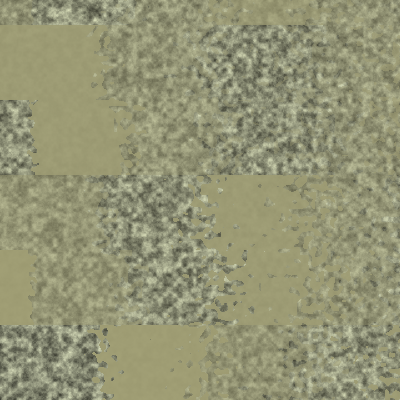
\includegraphics[width=\linewidth]{img/evaluation/M3/random/SBL_Adam_random_final.png}
    \caption{Target $T_{32}$ using Adam.}
    \label{fig:M3SBLFinalRendersRandomAdam}
\end{subfigure}\hspace{0.7cm}
\begin{subfigure}[t]{.25\textwidth}
    \centering
    
\includegraphics[width=\linewidth]{img/evaluation/M3/real life/SBL_Adam_real_life_final.png}
    \caption{Target $T_{33}$ using Adam.}
    \label{fig:M3SBLFinalRendersRealLifeAdam}
\end{subfigure}
\vskip\baselineskip
\begin{subfigure}[t]{.25\textwidth}
    \centering
    
\includegraphics[width=\linewidth]{img/evaluation/M3/2 param/SBL_Adam_2param_final.png}
    \caption{Target $T_{31}$ using RMSprop.}
    \label{fig:M3SBLFinalRendersTwoParamRMSprop}
\end{subfigure}\hspace{0.7cm}
\begin{subfigure}[t]{.25\textwidth}
    \centering
    \includegraphics[width=\linewidth]{img/evaluation/M3/random/SBL_RMSprop_random_final.png}
    \caption{Target $T_{32}$ using RMSprop.}
    \label{fig:M3SBLFinalRendersRandomRMSprop}
\end{subfigure}\hspace{0.7cm}
\begin{subfigure}[t]{.25\textwidth}
    \centering
\includegraphics[width=\linewidth]{img/evaluation/M3/real life/SBL_RMSprop_real_life_final.png}
    \caption{Target $T_{33}$ using RMSprop.}
    \label{fig:M3SBLFinalRendersRealLifeRMSprop}
\end{subfigure}
\caption{The six rendered textures at the point of minimal loss for $M_3$ using SBL corresponding to the six plots in Figure \ref{fig:M3SBLData} with combinations of optimizers Adam or RMSprop and targets $T_{31}$, $T_{32}$ or $T_{33}$.}
\label{fig:M3SBLFinalRenders}
\end{figure}

\newpage
\subsection{Parameter Estimation using Neural Loss}

\begin{table}[!h]
\centering
\begin{tabular}{ccllllllll}
\textbf{}      &                   & \textbf{}          & \multicolumn{1}{l|}{}            & \multicolumn{2}{l|}{\textit{Adam}}                           & \multicolumn{2}{l|}{\textit{RMSprop}}                      & \multicolumn{2}{l|}{\textit{Neural Loss}}               \\
\textbf{$M_i$} & \textbf{$T_{ij}$} & \textbf{Optimizer} & \multicolumn{1}{l|}{\textbf{lr}} & \textbf{$\beta_1$} & \multicolumn{1}{l|}{\textbf{$\beta_2$}} & \textbf{$\alpha$} & \multicolumn{1}{l|}{\textbf{Momentum}} & \textbf{layers} & \multicolumn{1}{l|}{\textbf{weights}} \\ \hline
 $M_1$     & $T_{11}$   & Adam       & 0.15       & 0.5        & 0.999      &            &            & [0]        & [1.0]      \\
 $M_1$     & $T_{11}$   & RMSprop    & 0.09       &            &            & 0.9        & 0.0        & [0]        & [1.0]      \\
 $M_1$     & $T_{12}$   & Adam       & 0.05       & 0.7        & 0.999      &            &            & [0]        & [1.0]      \\
 $M_1$     & $T_{12}$   & RMSprop    & 0.05       &            &            & 0.9        & 0.0        & [0]        & [1.0]      \\
  $M_2$     & $T_{21}$   & Adam       & 0.04       & 0.9        & 0.999      &            &            & [0, 4]     & [1.0, 4.0] \\
 $M_2$     & $T_{21}$   & RMSprop    & 0.02       &            &            & 0.99       & 0.4        & [0]        & [1.0]      \\
 $M_2$     & $T_{22}$   & Adam       & 0.04       & 0.9        & 0.999      &            &            & [0]        & [1.0]      \\
 $M_2$     & $T_{22}$   & RMSprop    & 0.02       &            &            & 0.95       & 0.4        & [0]        & [1.0]      \\
  $M_3$     & $T_{31}$   & Adam       & 0.01       & 0.9        & 0.999      &            &            & [5]        & [1.0]      \\
 $M_3$     & $T_{31}$   & RMSprop    & 0.01       &            &            & 0.99       & 0.0        & [4]        & [1.0]      \\
 $M_3$     & $T_{32}$   & Adam       & 0.02       & 0.9        & 0.999      &            &            & [0]        & [1.0]      \\
 $M_3$     & $T_{32}$   & RMSprop    & 0.02       &            &            & 0.99       & 0.4        & [0]        & [1.0]      \\
 $M_3$     & $T_{33}$   & Adam       & 0.005      & 0.85       & 0.999      &            &            & [0, 2, 4]  & [1.0, 4.0, 4.0] \\
 $M_3$     & $T_{33}$   & RMSprop    & 0.003      &            &            & 0.95       & 0.3        & [0, 2]     & [1.0, 4.0] \\
\end{tabular}
\caption{Optimizer and loss settings when running gradient descent using Neural loss.}
\label{tab:NeuralLossOptimizerSettings}
\end{table}


The neural loss can be controlled via two parameters: \texttt{layers} which is used to specify layer indices to extract features from and \texttt{weights} which is a list of weights for each selected layer as explained in section \ref{sec:NeuralFeatureLoss}. In a Neural Network, specific features are picked up by the early layers close to the input while general features are found by layers closer to the output. This means that we want to extract features from the early layers so as to not capture features that are too generic and experiments showed that features extracted from layers 0, 2, 4 and 5 generally give the most accurate results. Unlike MSE loss or SBL, the range of possible loss values greatly depends on choice of layers and weights, which makes it more difficult to judge whether the returned loss value is an objectively good result. In these experiments, we will therefore not set a threshold (except for $M_1$), but instead run gradient descent for 400 iterations and compare the initial loss to the minimum loss as well as subjectively judging the resulting rendered textures. The optimizer and loss settings used in each experiment with a neural loss is displayed in table \ref{tab:NeuralLossOptimizerSettings}.

\subsubsection{HSV Test Shader $M_1$}


Using a neural loss for uniform images of a single color without any patterns is not only considerably slower than using a simple MSE or SB loss, but did in this example yield less accurate results. For all runs with shader $M_1$ we only extract features from the first layer and use a weight of $1.0$. For the easier target $T_{11}$ we could keep the learning rate relatively high, but had to lower it for target $T_{12}$ to prevent oscillation. The results are shown in Figure \ref{fig:M1NeuralData} where the loss threshold was set to $0.05$, an arbitrary value judged to be low enough considering the high initial loss of almost $7.0$. Yet again, RMSprop outperforms Adam for both targets and reaches the threshold two or three iterations earlier. The best loss renders are shown in Figure \ref{fig:M1NeuralFinalRenders}, where we see that target $T_{11}$ was successfully reproduced with a very high similarity. For target $T_{12}$ however, the same loss threshold did not result in an equally accurate render, where the brown color is too light. This shows how the neural loss value is not as reliable as in the case of MSE loss or SBL and is not the best loss function to use with simple shaders like $M_1$ lacking patterns, being both slower and less accurate.

\begin{figure}[hpt]
    \centering
    \includegraphics[width=0.8\textwidth]{img/evaluation/M1/HSV_NEURAL.pdf}
    \caption{Results of evaluating parameter estimation of material $M_1$ using Neural loss. The runs with target $T_{11}$ are plotted as solid lines and target $T_{12}$ with dashed lines.}
    \label{fig:M1NeuralData}
\end{figure}

\begin{figure}[hpb]
\centering
\begin{subfigure}[t]{.25\textwidth}
    \centering
    \includegraphics[width=\linewidth]{img/evaluation/M1/2 param/Neural_Adam_final_render.png}
    \caption{Target $T_{11}$ using Adam.}
    \label{fig:M1NeuralFinalRenders2paramAdam}
\end{subfigure}\hspace{0.7cm}
\begin{subfigure}[t]{.25\textwidth}
    \centering
    \includegraphics[width=\linewidth]{img/evaluation/M1/random/Neural_Adam_random_final.png}
    \caption{Target $T_{12}$ using Adam.}
    \label{fig:M1NeuralFinalRendersRandomAdam}
\end{subfigure}
\vskip\baselineskip
\begin{subfigure}[t]{.25\textwidth}
    \centering
    \includegraphics[width=\linewidth]{img/evaluation/M1/2 param/Neural_RMSprop_final_render.png}
    \caption{Target $T_{11}$ using RMSprop.}
    \label{fig:M1NeuralFinalRenders2paramRMSprop}
\end{subfigure}\hspace{0.7cm}
\begin{subfigure}[t]{.25\textwidth}
    \centering
    \includegraphics[width=\linewidth]{img/evaluation/M1/random/Neural_RMSprop_random_final.png}
    \caption{Target $T_{12}$ using RMSprop.}
    \label{fig:M1NeuralFinalRendersRandomRMSprop}
\end{subfigure}
\caption{The four rendered textures at the point of minimal loss for $M_1$ using Neural loss corresponding to the four plots in Figure \ref{fig:M1NeuralData} with combinations of optimizers Adam or RMSprop and targets $T_{11}$ or $T_{12}$.}
\label{fig:M1NeuralFinalRenders}
\end{figure}

\subsubsection{Simple Brick Shader $M_2$}

The results of running gradient descent on test shader $M_2$ using a neural loss function are shown in Figure \ref{fig:M2NeuralData} where the initial loss when running parameter estimation using Adam with target $T_{21}$ is relatively high. As shown in table \ref{tab:NeuralLossOptimizerSettings}, we used a different set of layers to extract features from when running with target $T_{21}$ using Adam, which is reflected in Figure \ref{fig:M2NeuralData}, as it yielded much better results. It is interesting that the single layer 0 works well for RMSprop, but gave very poor results with Adam. This is probably due to RMSprop by chance finding a better path to a minimum and we could have probably reached the same results with Adam had we explored a much wider range of optimizer settings. Using Adam and target $T_{21}$ we were able to reach a minimum loss of $0.07$ at iteration 341 and with RMSprop a minimum loss of $0.004$ at iteration 334. The renders at these points of minimal loss are shown in subfigures \ref{fig:M2NeuralFinalRenders2paramAdam} and \ref{fig:M2NeuralFinalRenders2paramRMSprop} respectively where a slightly better result was achieved by using RMSprop but is surprisingly not much better than using a simple MSE loss. The color was retrieved fairly well but the elongation is only about 60\% of the target. The real advantage of using a neural loss is instead reflected in the cases with the random target $T_{22}$ where the initial loss starts at around $0.3$ and is minimized down to $0.02$ for Adam at iteration 381 and $0.036$ for RMSprop at iteration 21. While RMSprop is clearly much faster to reach convergence, the results are better for Adam as seen in subfigures \ref{fig:M2NeuralFinalRendersRandomRMSprop} and \ref{fig:M2NeuralFinalRendersRandomAdam} respectively. As opposed to using a MSE loss or SBL the shape of the bricks were actually retained and even elongated when using Adam, although not nearly as much as in the target. Clearly a neural loss is a better choice for pattern heavy images, especially when optimizing a large number of parameters, although it is still difficult to reproduce the exact shape.

\begin{figure}[h]
    \centering
    \includegraphics[width=0.8\textwidth]{img/evaluation/M2/SBS_Neural.pdf}
    \caption{Results of evaluating parameter estimation of material $M_2$ using Neural loss. The runs with target $T_{21}$ are plotted as solid lines while runs with target $T_{22}$ are plotted with dashed lines.}
    \label{fig:M2NeuralData}
\end{figure}

\begin{figure}[h]
\centering
\begin{subfigure}[t]{.25\textwidth}
    \centering
    \includegraphics[width=\linewidth]{img/evaluation/M2/2param/Neural_Adam_final_render.png}
    \caption{Target $T_{21}$ using Adam.}
    \label{fig:M2NeuralFinalRenders2paramAdam}
\end{subfigure}\hspace{0.5cm}
\begin{subfigure}[t]{.25\textwidth}
    \centering
    \includegraphics[width=\linewidth]{img/evaluation/M2/random/Neural_Adam_Random_best.png}
    \caption{Target $T_{22}$ using Adam.}
    \label{fig:M2NeuralFinalRendersRandomAdam}
\end{subfigure}
\vskip\baselineskip
\begin{subfigure}[t]{.25\textwidth}
    \centering
    \includegraphics[width=\linewidth]{img/evaluation/M2/2param/Neural_RMSprop_final_render.png}
    \caption{Target $T_{21}$ using RMSprop.}
    \label{fig:M2NeuralFinalRenders2paramRMSprop}
\end{subfigure}
\hspace{0.5cm}
\begin{subfigure}[t]{.25\textwidth}
    \centering
    \includegraphics[width=\linewidth]{img/evaluation/M2/random/Neural_RMSprop_Random_best.png}
    \caption{Target $T_{22}$ using RMSprop.}
    \label{fig:M2NeuralFinalRendersRandomRMSprop}
\end{subfigure}
\caption{The four rendered textures at the point of minimal loss for $M_2$ using Neural corresponding to the six plots in Figure \ref{fig:M2NeuralData} with combinations of optimizers Adam or RMSprop and targets $T_{21}$ or $T_{32}$.}
\label{fig:M2NeuralFinalRenders}
\end{figure}


\subsubsection{Advanced Brick Test Shader $M_3$}

\begin{figure}[h]
    \centering
    \includegraphics[width=0.8\textwidth]{img/evaluation/M3/ABS_NEURAL.pdf}
    \caption{Results of evaluating parameter estimation of material $M_3$ using Neural loss. The runs with target $T_{31}$ are plotted as solid lines, target $T_{32}$ with dashed lines and the additional real-life target $T_{33}$ with dotted lines.}
    \label{fig:M3NeuralData}
\end{figure}

\begin{figure}[h]
\centering
\begin{subfigure}[t]{.25\textwidth}
    \centering
    \includegraphics[width=\linewidth]{img/evaluation/M3/2 param/Neural_Adam_2_param.png}
    \caption{Target $T_{31}$ using Adam.}
    \label{fig:M3NeuralFinalRendersTwoParamAdam}
\end{subfigure}\hspace{0.7cm}
\begin{subfigure}[t]{.25\textwidth}
    \centering
    \includegraphics[width=\linewidth]{img/evaluation/M3/random/Neural_Adam_random_final.png}
    \caption{Target $T_{32}$ using Adam.}
    \label{fig:M3NeuralFinalRendersRandomAdam}
\end{subfigure}\hspace{0.7cm}
\begin{subfigure}[t]{.25\textwidth}
    \centering
    \includegraphics[width=\linewidth]{img/evaluation/M3/real life/Neural_Adam_real_life_final.png}
    \caption{Target $T_{33}$ using Adam.}
    \label{fig:M3NeuralFinalRendersRealLifeAdam}
\end{subfigure}
\vskip\baselineskip
\begin{subfigure}[t]{.25\textwidth}
    \centering
    \includegraphics[width=\linewidth]{img/evaluation/M3/2 param/Neural_RMSprop_2_param.png}
    \caption{Target $T_{31}$ using RMSprop.}
    \label{fig:M3NeuralFinalRendersTwoParamRMSprop}
\end{subfigure}\hspace{0.7cm}
\begin{subfigure}[t]{.25\textwidth}
    \centering
    \includegraphics[width=\linewidth]{img/evaluation/M3/random/Neural_RMSprop_random_final.png}
    \caption{Target $T_{32}$ using RMSprop.}
    \label{fig:M3NeuralFinalRendersRandomRMSprop}
\end{subfigure}\hspace{0.7cm}
\begin{subfigure}[t]{.25\textwidth}
    \centering
    \includegraphics[width=\linewidth]{img/evaluation/M3/real life/Neural_RMSprop_real_life_final.png}
    \caption{Target $T_{33}$ using RMSprop.}
    \label{fig:M3NeuralFinalRendersRealLifeRMSprop}
\end{subfigure}
\caption{The six rendered textures at the point of minimal loss for $M_3$ using Neural loss corresponding to the six plots in Figure \ref{fig:M3NeuralData} with combinations of optimizers Adam or RMSprop and targets $T_{31}$, $T_{32}$ or $T_{33}$.}
\label{fig:M3NeuralFinalRenders}
\end{figure}

Finally, we evaluate parameter estimation on $M_3$ using a neural loss function where the loss data is shown in Figure \ref{fig:M3NeuralData}. As seen in table \ref{tab:NeuralLossOptimizerSettings}, this case necessitated the use of a range of different settings for the neural loss function. Interestingly enough, there were big differences in performances between the two optimizers depending on which layers were used. Most notably for target $T_{31}$, where the same learning rate was used for both optimizers, but we only used layer $4$ for RMSprop and only layer $5$ for Adam as the reverse resulted in both optimizers performing much worse. The loss per iteration for $T_{31}$ is plotted using solid lines, and we can recognize a familiar pattern: RMSprop converges much earlier than Adam with a minimum loss of $0.0014$ at iteration 164 while Adam reaches a minimum loss of $0.009$ at iteration 397. Note that we can not directly compare the final loss values as we use different layers but the final renders shown in subfigures \ref{fig:M3NeuralFinalRendersTwoParamAdam} and \ref{fig:M3NeuralFinalRendersTwoParamRMSprop} respectively makes it clear that the result for Adam is superior. Both optimizers successfully retain the overall color of the target, but only Adam manages to correctly retain the scale, albeit at the expense of correct brick elongation. 

The loss data for the random target $T_{32}$ is plotted using dashed lines where both optimizers experience a fairly unstable few initial iterations. However, in this case RMSprop not only converges much earlier at iteration 192 versus Adam that does not converge at all, the minimum loss for RMSprop is much lower at $0.05$ against $0.13$ for Adam where both used layer $0$ with the same weights for the neural loss. Judging the resulting renders in subfigures \ref{fig:M3NeuralFinalRendersRandomAdam} for Adam and \ref{fig:M3NeuralFinalRendersRandomRMSprop} for RMSprop however, its difficult to see much similarity between either and the target.

The last and perhaps most interesting target $T_{33}$ is represented as dotted line plots where the additional layer $4$ was used for Adam which did not seem to provide any benefits for RMSprop. Both manage to quite successfully minimize the loss where Adam reached a minimum value of $0.2$ at iteration 363 and RMS a minimum value of $0.19$ at iteration 340. Furthermore, Adam experienced a much smoother progression whereas RMSprop saw several large spikes which might be preventable with better tuned learning rate and $\alpha$ parameters. The rendered results are shown in subfigures \ref{fig:M3NeuralFinalRendersRealLifeAdam} and \ref{fig:M3NeuralFinalRendersRealLifeRMSprop}, proving that the overall color has been very well reproduced in both cases, even the color of the mortar. What differentiates both cases is the scale of the bricks, where Adam managed to achieve better similarity, but again, both results show too elongated bricks. Furthermore, the noise function influencing the color of the bricks has not been changed much, although that could be the fault of the shader model composition itself. Ultimately, using a real life texture worked well but required a fair amount of tuning of optimizer and loss parameters.

Overall, the results are much better than when using MSE loss or SBL and except for target $T_{32}$, the overall color was very well retained, and when using Adam even the scale of the bricks was fairly well restored, although the elongation of the bricks remains a difficult problem to solve for both optimizers. For this case, Adam is the superior optimizer, although only marginally.


\subsection{Finding a ''Correct'' Minimum}

We have demonstrated that using gradient descent and a differentiable rendering system we can easily minimize a loss function applied to a static bitmap target and a generated image. However, there are no guarantees that the minimum found is a global minimum, or even that a low loss value corresponds to a high image similarity. In the end, the similarity is judged by a human user with a subjective idea of what constitutes similar images. Using a neural loss function is a big step in the right direction but in order to make judgements for other kinds of shaders, further evaluation is needed.

We impose practical limits on parameter values when controlled by the user, which can introduce problems during parameter estimation. For example, the hue, value and saturation parameters of the HSV shader are all limited to the interval $[0,1]$. The reason being that the hue parameter is cyclical meaning a value of 1.5 is equivalent to 0.5 while the saturation and value parameters are effectively capped to the interval so that a negative value is equivalent to 0 and any value > 1 is equivalent to 1. PyTorch tensors do not support such limits and neither do the optimizers. It would be possible to develop a custom optimizer that clamps parameters to their intervals, but this will inevitably have a negative impact on the optimization as a whole. Figure \ref{fig:HSVShaderLossSurface} shows the loss surface generated by evaluating the MSE loss of shader $M_1$ over a range of hue and saturation values using target $T_{11}$, as well as the gradient descent progress. A magenta plus symbol marks the minimum loss value and markers along the gradient descent route indicates each iteration. This proves the cyclic behaviour of the hue value as the loss is repeated along the x-axis. This means that we have one minimum every \texttt{hue=0.3,1.3,2.3} etc and because the initial value of the hue is 1.0, the closest minimum for the optimizer to seek is the one where \texttt{hue=1.3}, which unfortunately is outside of our limits, and simply clamping this value would result in a worse loss with \texttt{hue=1.0}.

\begin{figure}[h]
    \centering
    \includegraphics[width=0.8\textwidth]{img/evaluation/HSV Shader Loss Surface.pdf}
    \caption{Loss surface generated by evaluating an MSE loss between shader $M_1$ and target $T_{11}$ for a range of different \texttt{hue} and \texttt{value} parameter values. A magenta ''plus'' symbol denotes the point of minimum loss and the red line marks the gradient descent progress.}
    \label{fig:HSVShaderLossSurface}
\end{figure}


\chapter{Conclusion}
\textbf{Summarize Results and discussion}

\section{Future Work}

\textbf{PyTorch3D}
 
% Should use consistent formatting when it comes to Names ("FirstName LastName", or "F. LastName")
%\printbibliography
\makebibliography{MyBib}

\begin{appendices}
\chapter{Appendix A}

\checkoddpage
\ifoddpage
\else
   \newpage
   \thispagestyle{empty}
   \mbox{ }
\fi


\end{appendices}

\end{document}